\documentclass[12pt,twoside]{article}
%\usepackage[bottom]{draftcopy}
\usepackage{fancyvrb}
\usepackage{makeidx}      % for the index
\usepackage{graphicx}
%\usepackage{psfig}
\usepackage{amsmath}
\usepackage{eepic}        % for graphics, especially the \ellipse command
\usepackage{longtable}    % for multi-page tables
%\usepackage{subfigure}    % for multi-figure figures
\usepackage{html}  % sty that comes with the latex2html program
\usepackage{multicol}  % only used in the distribution page
\usepackage{tabularx}
%\usepackage[toc,page]{appendix}
\usepackage{hyperref}  % keep this last

\makeindex


\begin{document}
    
% Setup for letter paper with SAND report spacings and margins
\setlength{\textwidth}{6in}
\setlength{\oddsidemargin}{0.5in}
\setlength{\evensidemargin}{0.0in}
\setlength{\marginparwidth}{1.0in}
\addtolength{\marginparwidth}{-\marginparsep}
\setlength{\textheight}{9in}
\addtolength{\textheight}{-\footskip}
\addtolength{\textheight}{-\headheight}
\addtolength{\textheight}{-\headsep}
\setlength{\topmargin}{0.0in}
\setlength{\parskip}{2ex}

\newcommand{\makearticle}{
  \date{}
  \maketitle
}

\newcommand{\CoverFont}[3]{
    \fontencoding{OT1}
    \fontfamily{phv}
    \fontseries{#1}
    \fontshape{n}
    \fontsize{#2}{#3}
    \selectfont
}

\newcommand{\SANDreleaseval}{Unlimited Release}
\newcommand{\SANDrelease}[1]{\renewcommand{\SANDreleaseval}{#1}}

\newcommand{\SANDsupersedVar}{\\}
\newcommand{\SANDsupersedBox}{}
\newlength{\adjustsupersed}
\setlength{\adjustsupersed}{1.0in}
\newcommand{\SANDsupersed}[2]{
    \renewcommand{\SANDsupersedVar}{
        \vspace{0.125in}\\
        Supersedes #1 \\
        dated #2
    }
    \renewcommand{\SANDsupersedBox}{
      \mbox{\begin{tabular}{c}
              Supersedes #1 \\
              dated #2
            \end{tabular}}
    }
    \setlength{\adjustsupersed}{1.5in}
}

\newcommand{\makeSANDreport}[3]{

    % Some measurements to format the title page properly
    \newlength{\textwidththird}
    \newlength{\topheight}
    \newlength{\topleftwidth}
    \newlength{\topmiddlewidth}
    \newlength{\toprightwidth}
    \setlength{\textwidththird}{2in}
    \addtolength{\textwidththird}{-\fboxsep}
    \addtolength{\textwidththird}{-\fboxsep}
    \setlength{\topleftwidth}{\the\textwidththird}
    \setlength{\topmiddlewidth}{\the\textwidththird}
    \setlength{\toprightwidth}{\the\textwidththird}
    \addtolength{\topleftwidth}{-3em}
    \addtolength{\topmiddlewidth}{+4em}
    \addtolength{\toprightwidth}{-3em}

    % We want a blank line between paragraphs
    \setlength{\parskip}{2ex}

    {
        \pagestyle{empty}
        \newlength{\coverindent}
        \setlength{\coverindent}{1em}
        \setlength{\parindent}{0em}


        %
        % Front Cover
        %
        \addtolength{\headheight}{-0.625in}
        \hspace*{-0.5in}
        \begin{minipage}[t]{6.0in}
        {
        \CoverFont{b}{18}{20pt}
        SAND REPORT
        \vspace{0.125in}\\
        \CoverFont{m}{12}{14pt}
        #1\\
        \SANDreleaseval\\
        Printed #2
        \SANDsupersedVar

        \vspace{0.25in}
        \CoverFont{b}{24}{28pt}
        \parbox[t]{\textwidth}{
            \raggedright
            \thetitle
        }


        \vspace{0.75in}
        \CoverFont{m}{12}{14pt}
        #3

        \vspace{0.25in}
        \CoverFont{m}{8}{10pt}
        \selectfont
        Prepared by\\
        Sandia National Laboratories\\
        Albuquerque, New Mexico 87185 and Livermore, California 94550\\
        \\
        Sandia is a multiprogram laboratory operated by Sandia Corporation,\\
        a Lockheed Martin Company, for the United States Department of Energy's\\
        National Nuclear Security Administration under Contract DE-AC04-94-AL85000.\\
        \\
        Approved for public release; further dissemination unlimited.\\

        
\includegraphics{figures/snllineblk}
        }
        \end{minipage}

        %
        % Back cover
        %
        \newpage
        \hspace{1.0in}
        \begin{minipage}[t]{5.0in}
            \fontencoding{OT1}
            \fontfamily{pnc}
            \fontseries{m}
            \fontshape{n}
            \fontsize{9}{11pt}
            \selectfont

            Issued by Sandia National Laboratories, operated for the
            United States Department of Energy by Sandia Corporation.
            \vspace{\baselineskip}

            {\fontsize{11}{13pt}\fontseries{b}\selectfont NOTICE:}
            This report was prepared
            as an account of work sponsored by an agency of
            the United States Government. Neither the United
            States Government, nor any agency thereof, nor any
            of their employees, nor any of their contractors,
            subcontractors, or their employees, make any warranty,
            express or implied, or assume any legal liability or
            responsibility for the accuracy, completeness, or
            usefulness of any information, apparatus, product,
            or process disclosed, or represent that its use
            would not infringe privately owned rights. Reference
            herein to any specific commercial product, process,
            or service by trade name, trademark, manufacturer, or
            otherwise, does not necessarily constitute or imply
            its endorsement, recommendation, or favoring by the
            United States Government, any agency thereof, or any
            of their contractors or subcontractors. The views and
            opinions expressed herein do not necessarily state
            or reflect those of the United States Government,
            any agency thereof, or any of their contractors.
            \vspace{\baselineskip}

            Printed in the United States of America. This report has
            been reproduced directly from the best available copy.
            \vspace{\baselineskip}

            Available to DOE and DOE contractors from\\
            \begin{tabular}{ll}
                \hspace*{\coverindent} & U.S. Department of Energy \\
                & Office of Scientific and Technical Information \\
                & P.O. Box 62 \\
                & Oak Ridge, TN 37831 \\
                &  \\
            \end{tabular}
            \\
            \begin{tabular}{lll}
                \hspace*{\coverindent} & Telephone: & (865) 576-8401\\
                & Facsimile: & (865) 576-5728\\
                & E-Mail: &         reports@adonis.osti.gov\\
                & Online ordering: & http://www.doe.gov/bridge\\
            \end{tabular}
            \vspace{\baselineskip}
            \vspace{0.25in}

            Available to the public from\\
            \begin{tabular}{ll}
                \hspace*{\coverindent} & U.S. Department of Commerce \\
                & National Technical Information Service \\
                & 5285 Port Royal Rd \\
                & Springfield, VA 22161 \\
                &  \\
            \end{tabular}
            \\
            \begin{tabular}{lll}
                \hspace*{\coverindent} & Telephone: & (800) 553-6847 \\
                & Facsimile: & (703) 605-6900 \\
                & E-Mail: & orders@ntis.fedworld.gov \\
                & Online ordering: & http://www.ntis.gov/help/ordermethods.asp?loc=7-4-0\#online \\
            \end{tabular}
            \vspace{\baselineskip}
            \vspace{0.125in}

            
\includegraphics[width=0.75in]{figures/DOEbwlogo}
        \end{minipage}
        \newpage
        \addtolength{\headheight}{0.5in}
    }

  \date{}
  \newpage
  \begin{center}
      #1\\
      \SANDreleaseval\\
      Printed #2\\
      \bigskip
      \SANDsupersedBox
  \end{center}
  \bigskip

  \begin{center}
      \let \footnote \thanks
      {\LARGE \bf \thetitle\par}
      \vskip 1.5em
      {\large
          \lineskip .5em%
          \begin{tabular}[t]{c}
          \theauthor
          \end{tabular}\par
      }
  \end{center}
  \par
  \vskip 1.5em
}

\newcommand{\SANDdistInternal}[4]{
  \item[#1] MS \makebox[6ex][r]{#2}\\
    \mbox{}
    \hspace{1em} \parbox[t]{2.0in}{#3, \mbox{#4}}
}

\newcommand{\SANDdistExternal}[2]{
    \item[#1] \parbox[t]{2.1in}{#2}
}

%%%%%%%%%%%%%%%%%%%%%%%%%%%%%%%%%%%%%%%%%%%%%%%%%%%%%%%%%%%

%vectors
\newcommand{\E}{\overrightarrow {E}}
\newcommand{\B}{\bf{B}}
\newcommand{\Jb}{\overrightarrow {J}}
\newcommand{\A}{\overrightarrow {A}}
\newcommand{\jv}{\overrightarrow {j}}
\newcommand{\vv}{\overrightarrow {v}}

%vector operators
\newcommand{\del}{\nabla}
\newcommand{\lap}{\nabla^2}
\newcommand{\deld}{\del \cdot}
\newcommand{\curl}{\del \times}
\newcommand{\vxB}{\vv \times \B}

%partial derivatives
\newcommand{\dBdt}{\frac{\partial{\B}}{\partial{t}} }
\newcommand{\dBdx}{\frac{\partial{\B}}{\partial{x}} }
\newcommand{\dEdt}{\frac{\partial{\E}}{\partial{t}} }

%Equations
\newcommand{\beq}{\begin{equation}}
\newcommand{\eeq}{\end{equation}}
\newcommand{\beqn}{\begin{eqnarray*}}
\newcommand{\eeqn}{\end{eqnarray*}\beq \eeq }

\def \la{\langle}
\def \ra{\rangle}
\def \lp{\left(}
\def \rp{\right)}
\def \lb{\left[}
\def \rb{\right]}
\def \lc{\left\{}
\def \rc{\right\}}
\def \om{\omega}
\def \oom{\frac{1}{\omega}}
\def \ha{\frac{1}{2}}
\def \sA{{\bf A}}
\def \su{{\bf u}}
\def \sb{{\bf b}}
\def \sr{{\bf r}}
\def \pD{D^{(\pi)}}
\def \pC{C^{(\pi)}}
\def \pL{C_L^{(\pi)}}
\def \pU{C_U^{(\pi)}}

\def\bI{{\bf I}}
\def\bJ{{\bf J}}
\def\bA{{\bf A}}
\def\bE{{\bf E}}
\def\bD{{\bf D}}
\def\bB{{\bf B}}
\def\bH{{\bf H}}
\def\bS{{\bf S}}
\def\bT{{\bf T}}
\def\bv{{\bf v}}
\def\bx{{\bf x}}
\def\be{{\bf e}}
\def\ba{{\bf a}}
\def\Bf{{\bf f}}
\def\bg{{\bf g}}


\newcommand{\hf}{\frac{1}{2}}
%\newcommand{\ip1}{i+1}
%\newcommand{\im1}{i-1}
%\newcommand{\jp1}{j+1}
%\newcommand{\jm1}{j-1}

\newcommand{\HRule}{\rule{\linewidth}{1mm}}
\renewcommand{\theequation}{\thesection.\arabic{equation}}


% The altdescription environment is a modification of the description
% environment used to define math nomenclature, acronyms, etc.  Use
%    \begin{altdescription}{longest item}
%      \item{short item} blah blah
%      \item{longest item} blah blah
%    \end{altdescription}
% The argument is typically the longest typeset item value.  This environment
% takes an optional argument which is a length value. It adds length to the
% distance from the item values to their descirptions, such as 5em or 10pt.
%
\newenvironment{altdescription}[2][0pt]
  {\begin{list}{}%
    {\renewcommand\makelabel[1]{##1\hfil}%
     \settowidth\labelwidth{\makelabel{#2}}%
     \addtolength\labelwidth{#1}%
     \setlength\leftmargin{\labelwidth}%
     \addtolength\leftmargin{\labelsep}%
     \setlength\itemsep{-\parsep}}}%
  {\end{list}}


% The twocolumntable command is mainly used to hide the differences between
% the commands that produce nice output in PDF/DVI and in HTML.  Usage:
%   \twocolumntable{This is the caption text.\label{tablabel}}{
%     % put tabular environment here
%   }
% The first argument is the caption text, which should include the label.
% The second argument is the contents of the table.  An optional argument
% allows the column specification to be passed into the "tabularx"
% environment, which defaults to "|l|l|X|".
%
\latexhtml{
\newcommand{\twocolumntable}[3][|l|X|]%
  % use the column specifiers (if given) for PDF and DVI output
  {\begin{table}[ht]%
        \centering%
        \caption{#2}%
        \bigskip%
   \begin{tabularx}{\linewidth}{#1} #3 \end{tabularx}\end{table}}
}{
\newcommand{\twocolumntable}[3][|l|X|]%
  % do not use the column specifiers for latex2html output
  {\begin{table}[ht]%
        \begin{makeimage}\end{makeimage}%
        \centering%
        \caption{#2}%
        \bigskip%
   \begin{tabularx}{\linewidth}{|l|X|} #3 \end{tabularx}\end{table}}
}


% The threecolumntable command is mainly used to hide the differences between
% the commands that produce nice output in PDF/DVI and in HTML.  Usage:
%   \threecolumntable{This is the caption text.\label{tablabel}}{
%     % put tabular environment here
%   }
% The first argument is the caption text, which should include the label.
% The second argument is the contents of the table.  An optional argument
% allows the column specification to be passed into the "tabularx"
% environment, which defaults to "|l|l|X|".
%
\latexhtml{
\newcommand{\threecolumntable}[3][|l|l|X|]%
  % use the column specifiers (if given) for PDF and DVI output
  {\begin{table}[ht]%
        \centering%
        \caption{#2}%
        \bigskip%
   \begin{tabularx}{\linewidth}{#1} #3 \end{tabularx}\end{table}}
}{
\newcommand{\threecolumntable}[3][|l|l|X|]%
  % do not use the column specifiers for latex2html output
  {\begin{table}[ht]%
        \begin{makeimage}\end{makeimage}%
        \centering%
        \caption{#2}%
        \bigskip%
   \begin{tabularx}{\linewidth}{|l|l|X|} #3 \end{tabularx}\end{table}}
}

\latexhtml{
\newcommand{\mthreecolumntable}[3][|X|l|X|]%
  % use the column specifiers (if given) for PDF and DVI output
  {\begin{table}[ht]%
        \centering%
        \caption{#2}%
        \bigskip%
   \begin{tabularx}{\linewidth}{#1} #3 \end{tabularx}\end{table}}
}{
\newcommand{\mthreecolumntable}[3][|X|l|X|]%
  % do not use the column specifiers for latex2html output
  {\begin{table}[ht]%
        \begin{makeimage}\end{makeimage}%
        \centering%
        \caption{#2}%
        \bigskip%
   \begin{tabularx}{\linewidth}{|l|l|X|} #3 \end{tabularx}\end{table}}
}


% The fourcolumntable command is mainly used to hide the differences between
% the commands that produce nice output in PDF/DVI and in HTML.  Usage:
%   \fourcolumntable{This is the caption text.\label{tablabel}}{
%     % put tabular environment here
%   }
% The first argument is the caption text, which should include the label.
% The second argument is the contents of the table.  An optional argument
% allows the column specification to be passed into the "tabularx"
% environment, which defaults to "|l|l|l|X|".
%
\latexhtml{
\newcommand{\fourcolumntable}[3][|l|l|l|X|]%
  % use the column specifiers (if given) for PDF and DVI output
  {\begin{table}[ht]%
        \centering%
        \caption{#2}%
        \bigskip%
   \begin{tabularx}{\linewidth}{#1} #3 \end{tabularx}\end{table}}
}{
\newcommand{\fourcolumntable}[3][|l|l|l|X|]%
  % do not use the column specifiers for latex2html output
  {\begin{table}[ht]%
        \begin{makeimage}\end{makeimage}%
        \centering%
        \caption{#2}%
        \bigskip%
   \begin{tabularx}{\linewidth}{|l|l|l|X|} #3 \end{tabularx}\end{table}}
}


% The twocolumnlongtable command is mainly used to hide the differences
% between the commands that produce nice output in PDF/DVI and in HTML.  Usage:
%   \twocolumnlongtable{This is the caption text.\label{mytablelabel}}{
%     % tabular environment here
%   }
% The first argument is the caption text, which should include the label.
% The second argument is the contents of the table.  An optional argument
% allows the column specification to be passed into the "longtable"
% environment, which defaults to "|l|l|".
%
\latexhtml{
  % use longtable for PDF and DVI output
  \newcommand{\twocolumnlongtable}[3][|l|l|]%
 {\begin{longtable}{#1}%
     \caption{#2}%
  \endfirsthead%
     \hline%
     \multicolumn{2}{|l|}{\small\slshape continued from previous page} \\ \hline%
  \endhead%
     \multicolumn{2}{|r|}{\small\slshape continued on next page} \\ \hline%
  \endfoot%
     \hline%
  \endlastfoot%
  #3 %
  \end{longtable} }
}{
  % use table with tabularx for latex2html output
  \newcommand{\twocolumnlongtable}[3][|l|X|]%
 {\begin{table}[ht]%
    \begin{makeimage}  \end{makeimage}%
    \caption{#2}%
  \begin{tabularx}{\linewidth}{|l|X|}%
    \centering%
  #3 %
  \end{tabularx}\end{table} }
}


% The threecolumnlongtable command is mainly used to hide the differences
% between the commands that produce nice output in PDF/DVI and in HTML.  Usage:
%   \threecolumnlongtable{This is the caption text.\label{mytablelabel}}{
%     % tabular environment here
%   }
% The first argument is the caption text, which should include the label.
% The second argument is the contents of the table.  An optional argument
% allows the column specification to be passed into the "longtable"
% environment, which defaults to "|l|l|l|".
%
\latexhtml{
  % use longtable for PDF and DVI output
  \newcommand{\threecolumnlongtable}[3][|l|l|l|]%
 {\begin{longtable}{#1}%
     \caption{#2}%
  \endfirsthead%
     \hline%
     \multicolumn{3}{|l|}{\small\slshape continued from previous page} \\ \hline%
  \endhead%
     \multicolumn{3}{|r|}{\small\slshape continued on next page} \\ \hline%
  \endfoot%
     \hline%
  \endlastfoot%
  #3 %
  \end{longtable} }
}{
  % use table with tabularx for latex2html output
  \newcommand{\threecolumnlongtable}[3][|l|l|X|]%
 {\begin{table}[ht]%
    \begin{makeimage}  \end{makeimage}%
    \caption{#2}%
  \begin{tabularx}{\linewidth}{|l|l|X|}%
    \centering%
  #3 %
  \end{tabularx}\end{table} }
}


% The fourcolumnlongtable command is mainly used to hide the differences
% between the commands that produce nice output in PDF/DVI and in HTML.  Usage:
%   \fourcolumnlongtable{This is the caption text.\label{mytablelabel}}{
%     % tabular environment here
%   }
% The first argument is the caption text, which should include the label.
% The second argument is the contents of the table.  An optional argument
% allows the column specification to be passed into the "longtable"
% environment, which defaults to "|l|l|l|l|".
%
\latexhtml{
  % use longtable for PDF and DVI output
  \newcommand{\fourcolumnlongtable}[3][|l|l|l|l|]%
 {\begin{longtable}{#1}%
     \caption{#2}%
  \endfirsthead%
     \hline%
     \multicolumn{4}{|l|}{\small\slshape continued from previous page} \\ \hline%
  \endhead%
     \multicolumn{4}{|r|}{\small\slshape continued on next page} \\ \hline%
  \endfoot%
     \hline%
  \endlastfoot%
  #3 %
  \end{longtable} }
}{
  % use table with tabularx for latex2html output
  \newcommand{\fourcolumnlongtable}[3][|l|l|l|X|]%
 {\begin{table}[ht]%
    \begin{makeimage}  \end{makeimage}%
    \caption{#2}%
  \begin{tabularx}{\linewidth}{|l|l|l|X|}%
    \centering%
  #3 %
  \end{tabularx}\end{table} }
}


    \newcommand{\thetitle}{Pamgen, a Library for Parallel Generation of Simple Finite Element Meshes}
    \title{\thetitle}
    
    \newcommand{\theauthor}{ D. M. Hensinger, R. R. Drake, J. G. Foucar, T. A. Gardiner
       \\
       Sandia National Laboratories\\
       P.O. Box 5800\\
       Albuquerque, NM 87185-0378\\
    }
    \author{\theauthor}

    \latexhtml{
      %
      % SANDrelease defaults to Unlimited Release
      % use SANDsupersed if this report superseds a previous report
      %
      \SANDrelease{Unlimited Release}
      %\SANDsupersed{SAND2008-6541}{January 2008}
      \makeSANDreport{SAND2008-1933}{April 2008}
      {
          David M. Hensinger,
	  Richard R. Drake,
          James G. Foucar,
	  Thomas A. Gardiner
      }
    }{
      \makearticle
    }
    


% ---------------------------------------------------------------------------- %
    
    % An Abstract is required for SAND reports
    \begin{abstract}
Generating finite-element meshes is a serious bottleneck for
large parallel simulations. When mesh generation is limited to serial
machines and element counts approach a billion, this bottleneck becomes
a roadblock.  \textsc{pamgen} is a parallel mesh generation
library that allows on{}-the{}-fly scalable generation of hexahedral and quadrilateral finite
element meshes for several simple geometries. It has been used to
generate more that 1.1 billion elements on 17,576 processors. 

\textsc{pamgen} generates an unstructured finite element mesh on each processor at the start
of a simulation. The mesh is specified by commands passed to the library as a {}''C{}''-programming language string.  The resulting mesh geometry, topology, and communication information can then be queried through an API. \textsc{pamgen} allows specification of boundary condition application regions using 
sidesets (element faces) and nodesets (collections of nodes). It supports several simple geometry types. It has multiple alternatives
for mesh grading. It has several alternatives for the initial domain decompositon. \textsc{pamgen} makes it easy to change details of the finite element mesh and is very usesful for performance studies and scoping calculations.
    \end{abstract}


    % An Acknowledgement section is optional.
    % Use \section* since we don't want it in the table of context
    \clearpage
    \section*{Acknowledgment}
        The \textsc{pamgen} capabilities would not have been developed without the support and inspiration of the \textsc{alegra} community of users and developers. Within the users community, Chris Garasi and his challenging analysis requirements were the spur for development of the most complex and rewarding capabilities. Tom Brunner severely stressed the code with his early testing on large platforms. Within the developers community, the build and benchmark utilities written by Richard Drake enabled continual improvement in functionality and robustness. Tom Gardiner provided the code that is the heart of the default load balance capability.


    % reset
        \setcounter{table}{0}


    % Make sure this starts on an odd numbered page
  %  \clearpage
  %  \vspace*{\fill} \hspace*{\fill}
  %    This page intentionally left blank. \hspace*{\fill} \vspace*{\fill}
%
    \clearpage
    \tableofcontents
    
    
    % Comment out if there are no figures or tables.
    \clearpage
    \listoffigures

    \clearpage
    \listoftables


 
    \clearpage

    % ---------------------------------------------------------------------- %
    % This is where the body of the report begins
    
    \latex{\tolerance=1000}
    
    \section{Introduction}
To overcome the challenge of producing multi{}-million finite element
meshes for simulations using more than 1000 processors a library has been 
developed (\textsc{pamgen}) that for several simple geometries produces each processor's mesh as an early step of the analysis execution. The specification for these meshes is provided by a block of terse instructions that may be placed in an input file. These instructions are passed to the library as a {}''C{}''-programming language character array. \textsc{pamgen} is also referred to as an ``in line'' mesh generator because the meshing instructions may be included in one of the analysis input decks.

The simple input format allows analysts to change the resolution of 
a simulation by altering a few parameters. It also allows them to execute their simulations on
different numbers of processors without requiring any pre-processing.

The mesh generation proceeds through steps of decomposition, local
element creation, and communication information generation. The final
product of the library is a data structure that can be queried using an API (Application Programming Interface) that is based on the NEMESIS and EXODUS APIs. Currently the library
is limited to generating meshes of domains with cylindrical, tubular,
and block shapes. Substantial control is allowed over the element
density within these shapes. Boundary condition application  
regions can be specified on the surfaces and interior of the mesh .

Development of this capability revealed that the parallel mesh
generation process can be reduced to answering a series of questions:
What elements are on this processor? What nodes are on this processor?
What is the connectivity of this element? What elements border this
element? What processor does this element reside on?... Resolving these
questions inductively, without resolution to communication, is
essential for preserving scalability. Once a framework
for posing and answering these questions for a particular geometry is
established, expanding the capability to support additional geometries
is straightforward.

   
    

\clearpage
\section{Capabilities}\label{sec:caps}
The capabilities of \textsc{pamgen} are best understood by studying Section ~\ref{sec:specifying_a_mesh}, which documents in detail the instructions available for specifying a mesh. This section provides a brief overview of the library's capabilities. \textsc{pamgen} will be distributed as part of the \textsc{Trilinos} package of matrix and finite element tools.

\subsection{Dimensions}
\textsc{pamgen} can create both two and three dimensional meshes. It creates quadrilateral finite element meshes if two dimensions are specified, and it creates hexahedral finite element meshes if three dimensions are specified. For two dimensional quadrilateral meshes the Z component of nodal coordinates is not supplied.

\subsection{Mesh Geometries}

The \textsc{pamgen} library handles the mesh geometries shown below:
\begin{itemize}\addtolength{\itemsep}{-0.5\baselineskip}
\item Bricks
\item Partial hollow cylinders
\item Complete hollow cylinders
\item Partial solid cylinders
\item Complete solid cylinders
\end{itemize}


\begin{figure}[h]
    \centering
      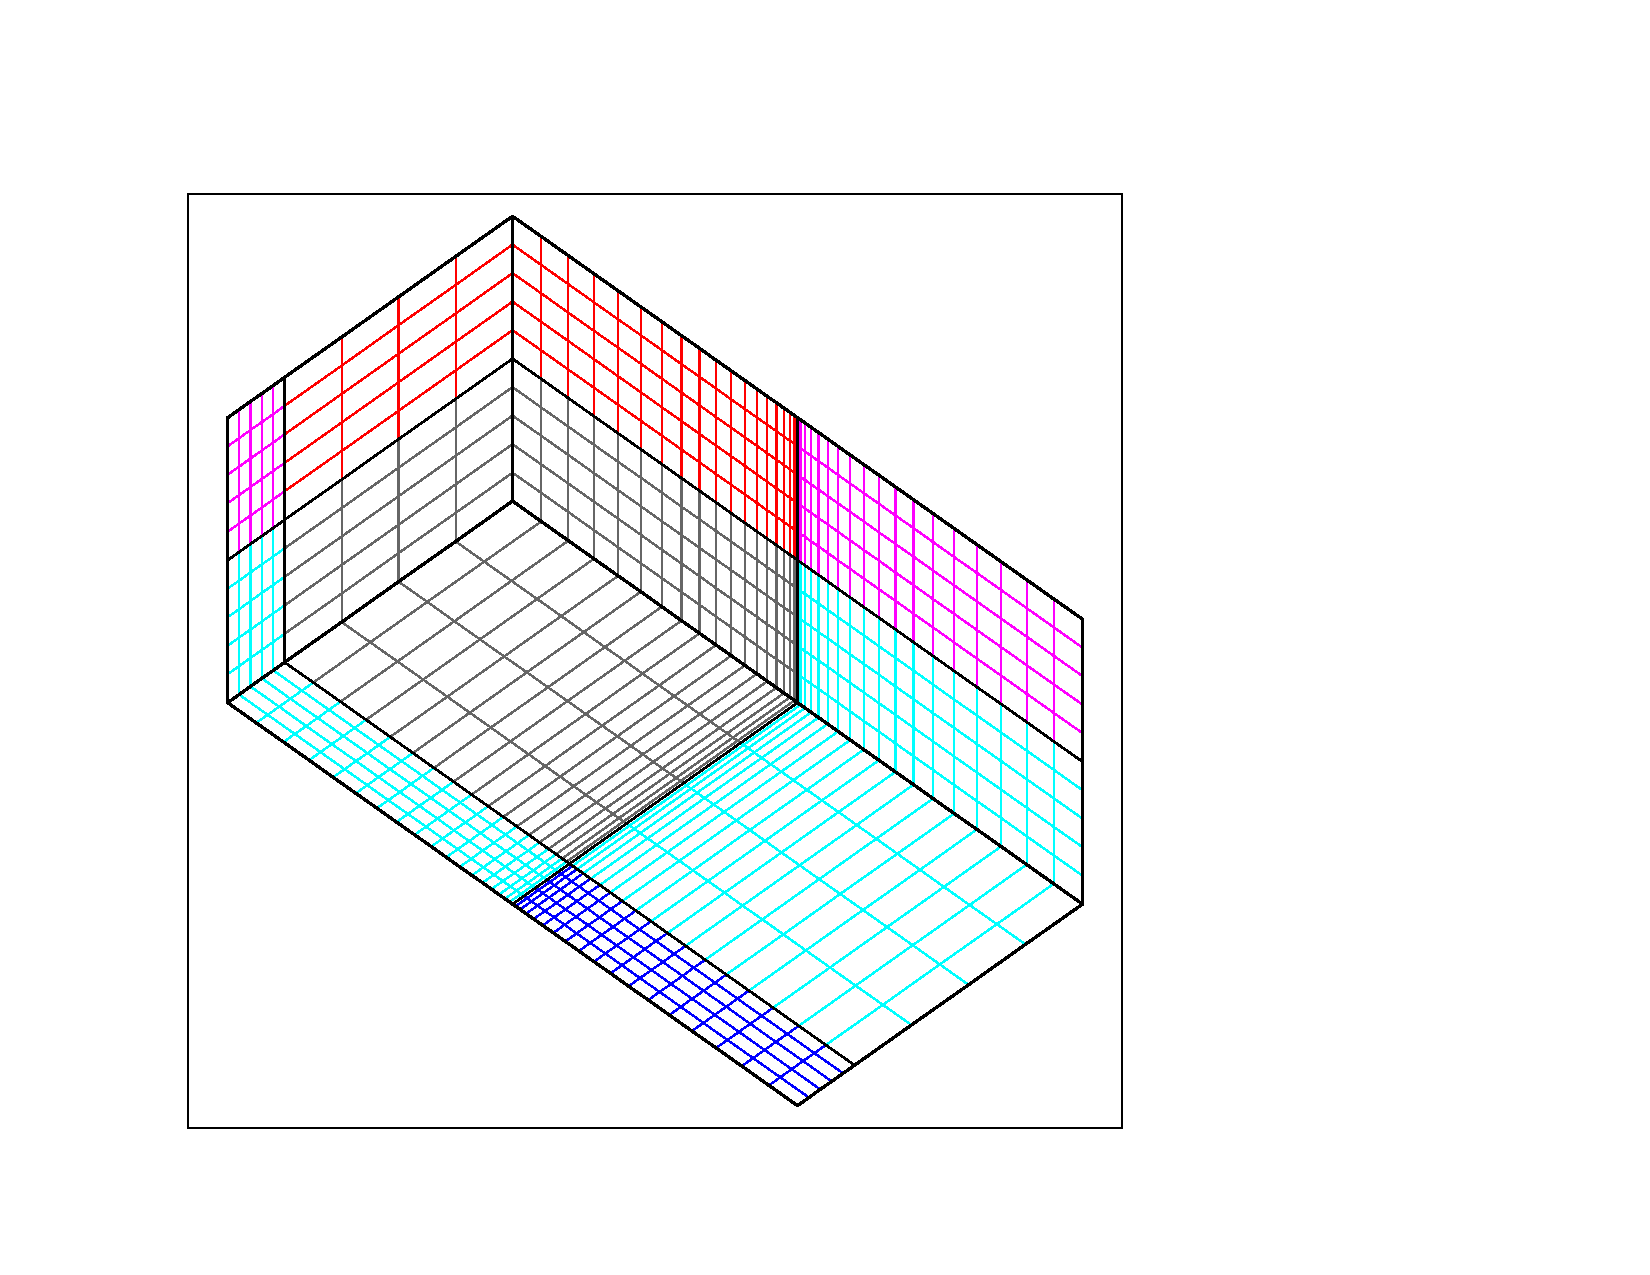
\includegraphics[width=1.0in]{figures/brick}
      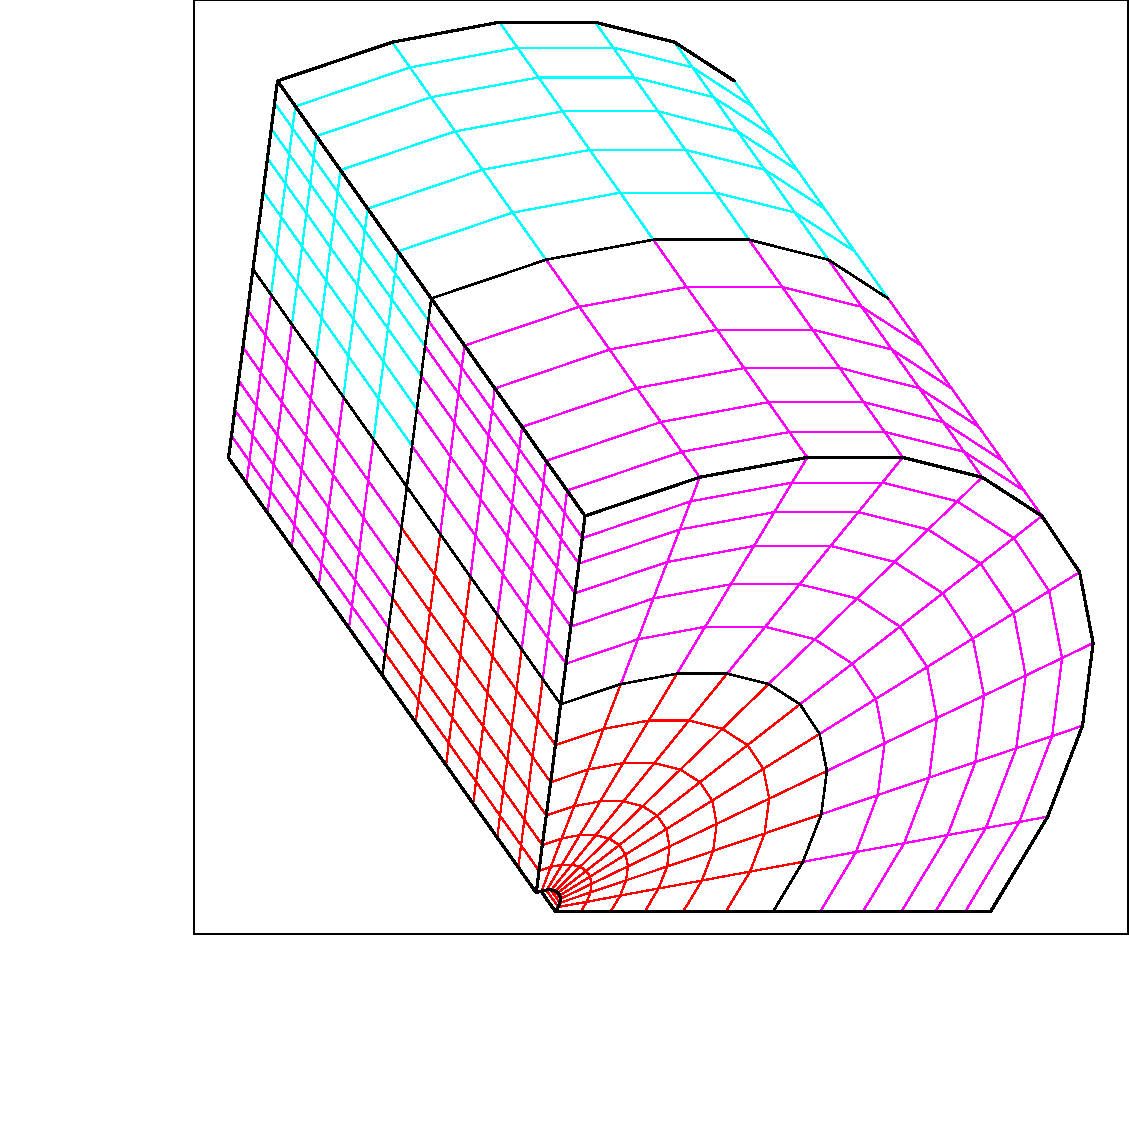
\includegraphics[width=1.0in]{figures/cubit_radial1}
      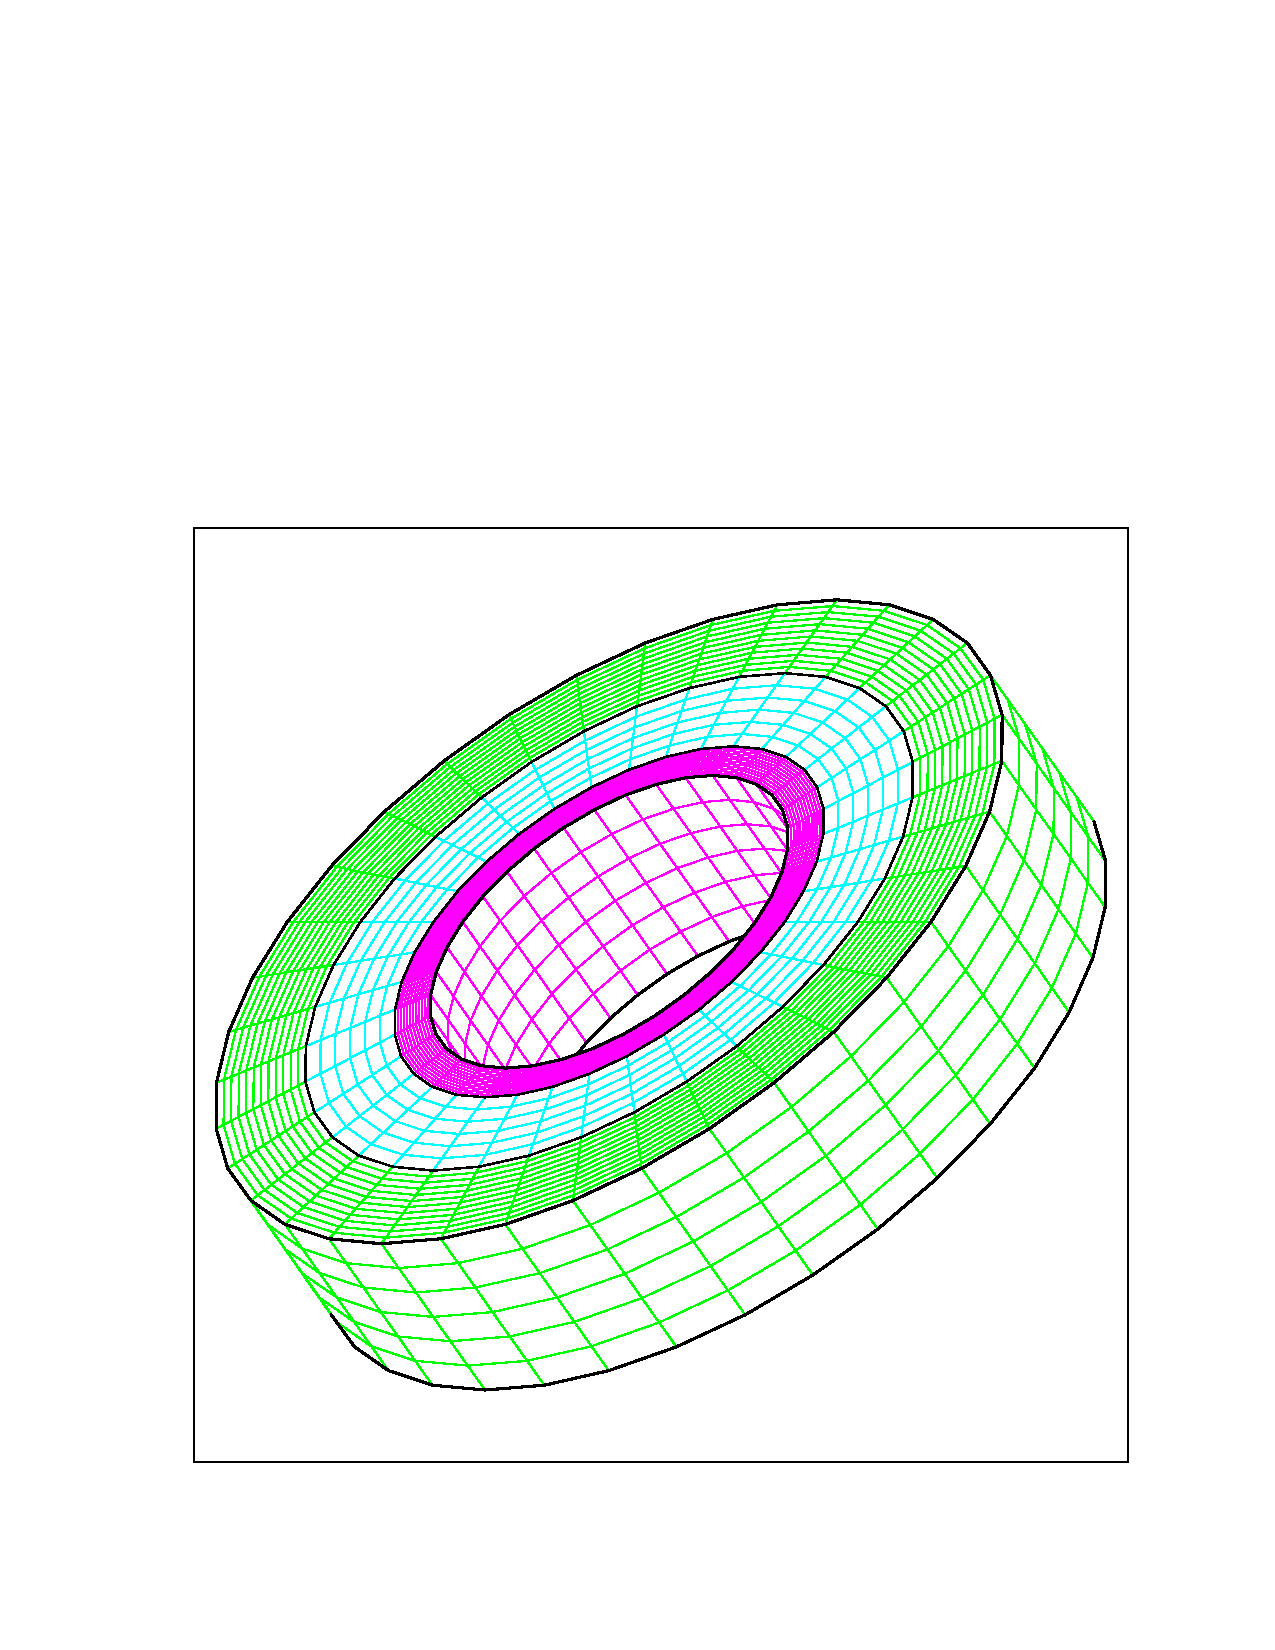
\includegraphics[width=1.0in]{figures/cubit_radial2}
      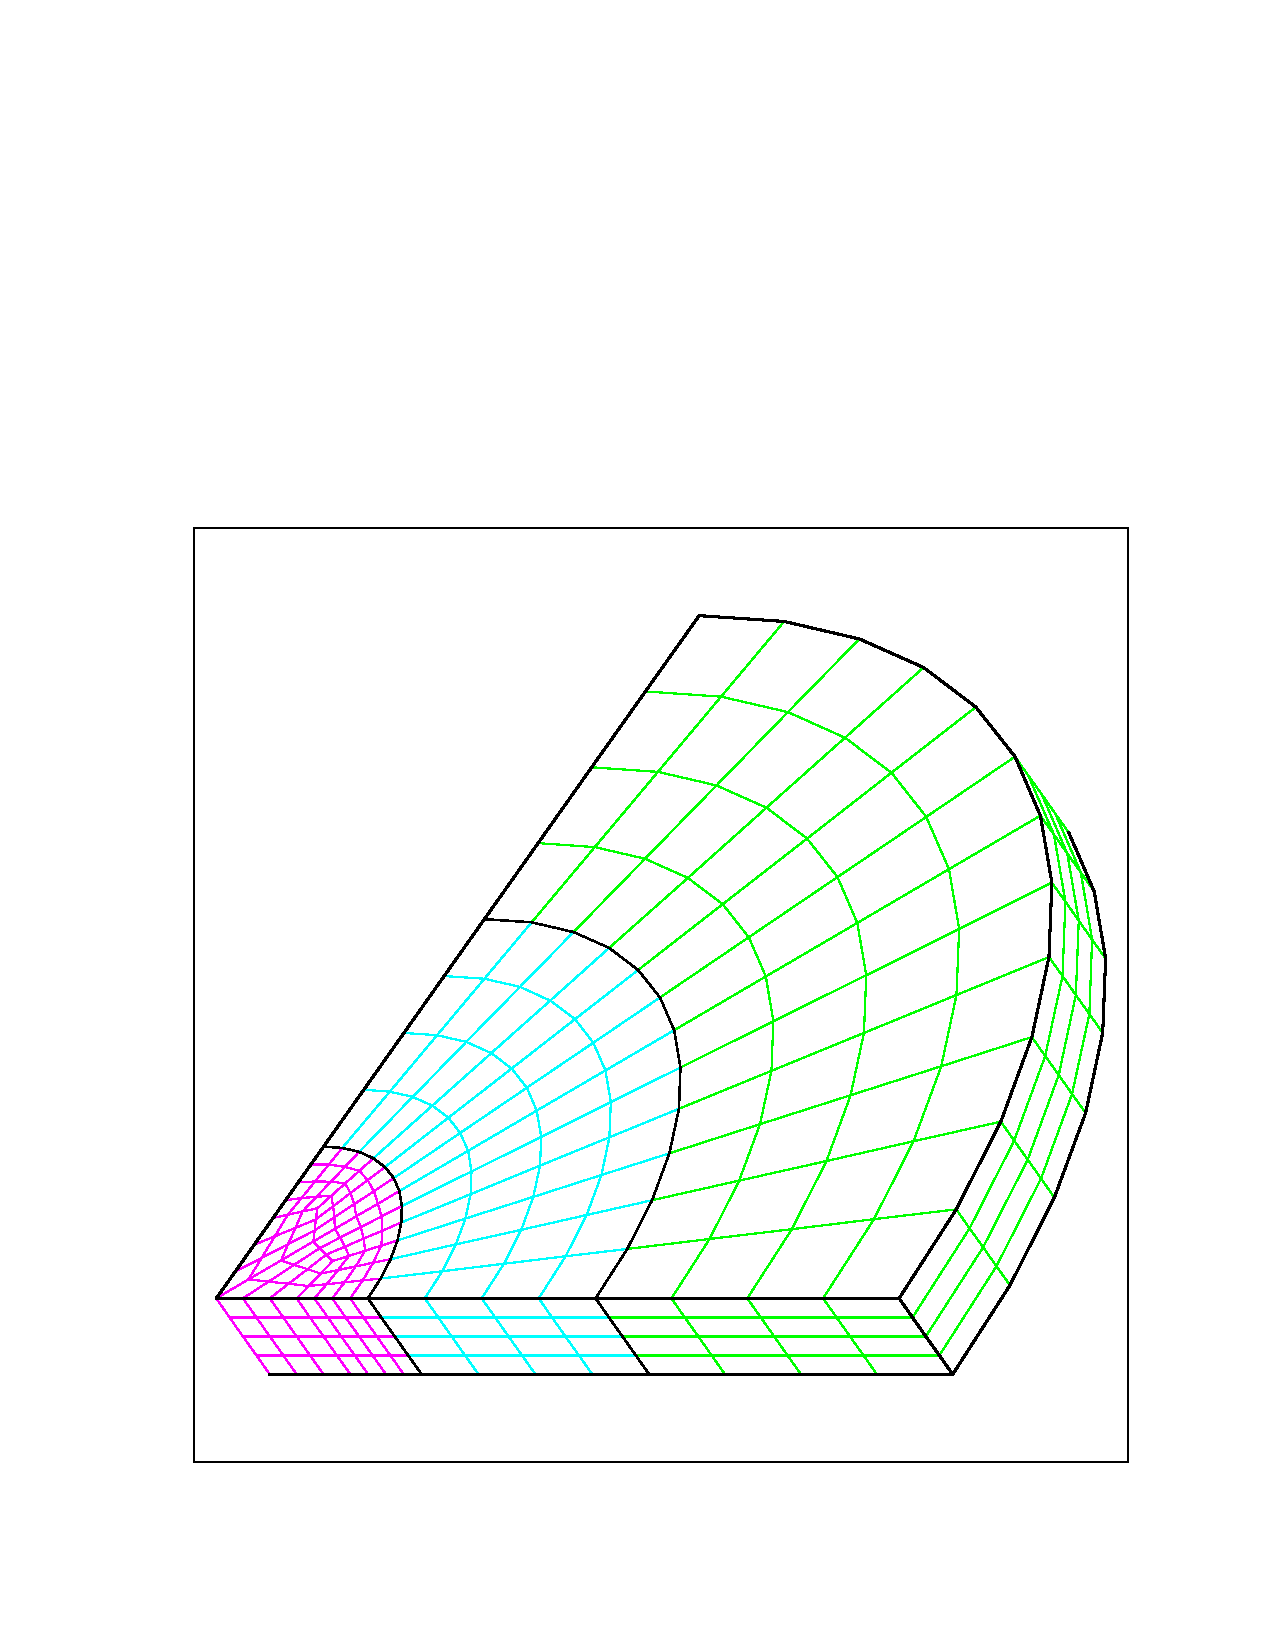
\includegraphics[width=1.0in]{figures/cubit_radial_trisection}
      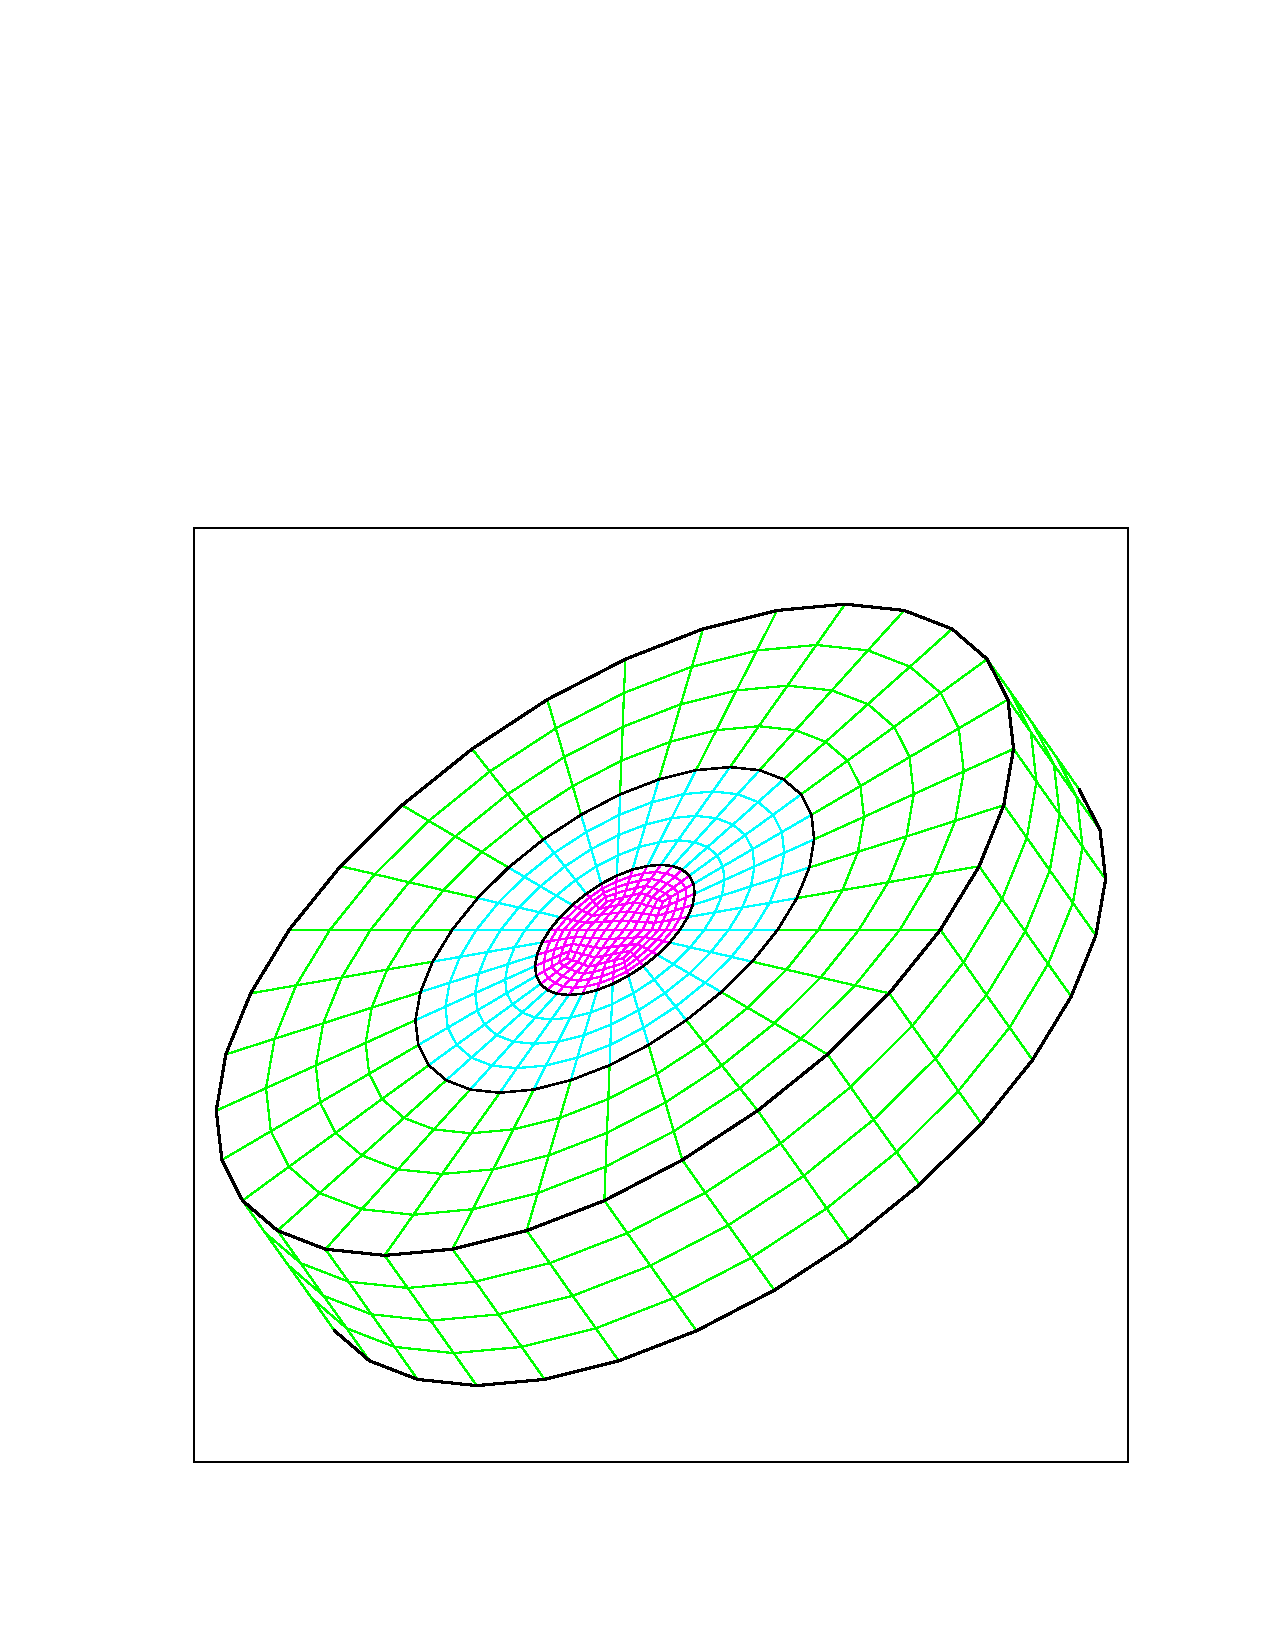
\includegraphics[width=1.0in]{figures/cubit_radial_trisection2}
  \caption{The mesh geometry zoo in 3D.}
  \label{fig:btm}
\end{figure}

\subsection{Boundary Conditions}
Boundary conditions application regions in the form of node sets and side sets can be applied to the face, edge, or corner of any element block in the finite element mesh. They may also be applied to any face, edge, or corner of the entire mesh.
\subsection{Decomposition}
There are several mesh decomposition strategies available in \textsc{pamgen}:
\begin{itemize}\addtolength{\itemsep}{-0.5\baselineskip}
\item A default decomposition based on a constrained optimized solution that slices through the entire mesh in its three (or two in 2D) topological dimensions.
\item A user defined slicing strategy that specifies the number of slices through the mesh in each topological direction.
\item A sequential strategy that distributes elements beetween processors based on their element ids with the first n  elements going to processor 0 ...
\item A random strategy that assigns element to processors randomly.
\end{itemize}

\subsection {Geometry Transformation}
Any mesh can be modified by re-evaluating the nodal coordinate values using a user-supplied function. This function has the original nodal coordinates as input values. Its output values define the new nodal coordinates.



\begin{figure}[h]
    \centering
      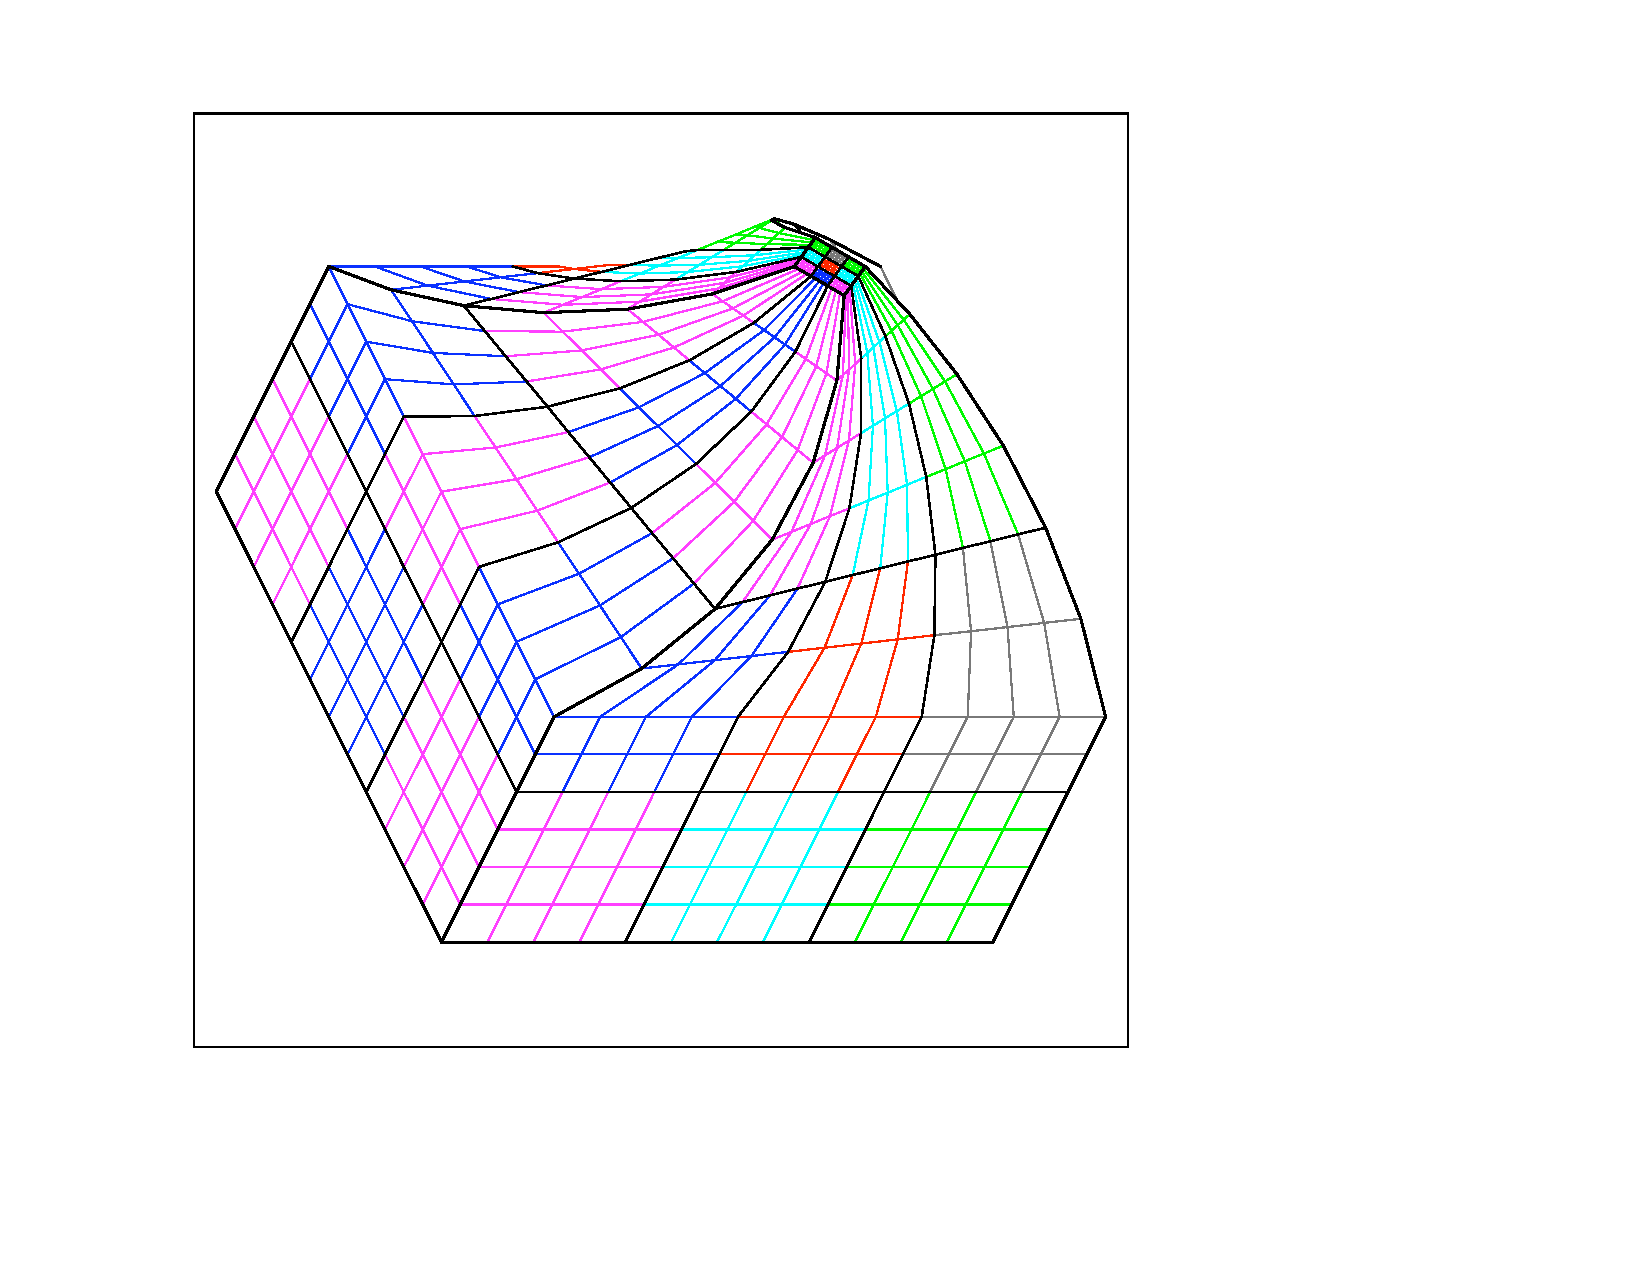
\includegraphics[width=1.0in]{figures/3d_warped_geometry_white_bg}
      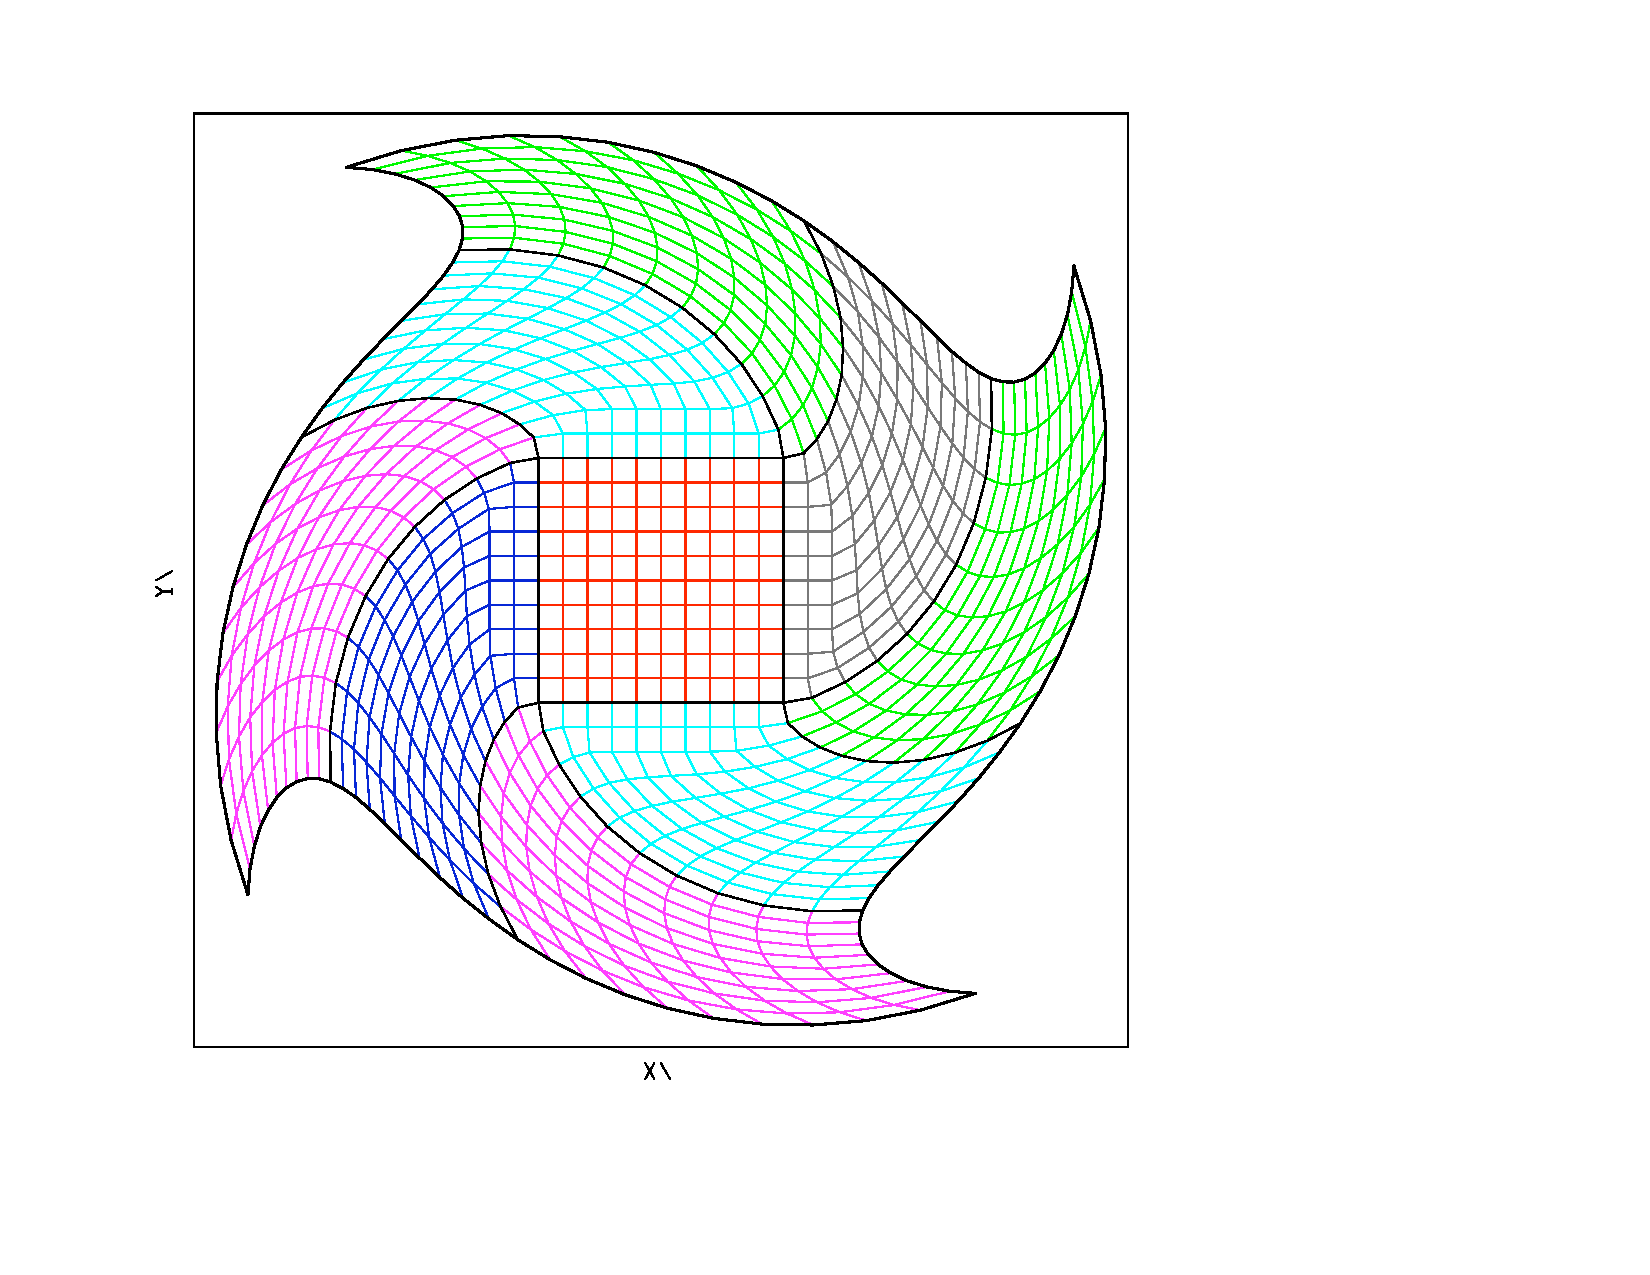
\includegraphics[width=1.0in]{figures/mesh_warp_2d_white_bg}
  \caption{Examples of geometry transformation.}
  \label{fig:btm}
\end{figure}


\subsection{Element Density}
Several of the geometry types allow specification of first and last element sizes within a block in a particular cartesian direction. In addition the user may control node distribution over any geometry by providing a user defined distribution function. This function is evaluated so that nodes are shifted towards areas where the function has its highest values.

\clearpage
\section{Approach}\label{sec:challenge}
\textsc{pamgen} operates on the premise that mesh generation is deterministic. This means that every execution of code compiled with compiler A and run on processor B under operating system C reading mesh instructions file D will produce an identical mesh. The mesh will have the same topology and the nodes will have the same coordinate locations.  On a multi-processor machine of identical nodes an arbitrary number of processors executing identical instructions produce an identical mesh. Use of \textsc{pamgen} on heterogeneous machines may produce unexpected results.

With one significant exception, \textsc{pamgen} operates in the same way as these identical processors producing identical mesh. The exception is that each processor only allocates for a subset of the nodes and elements, and each processor performs topology and geometry calculations only for the entities and dependencies present on that processor.  \textsc{pamgen} exploits the fact that each processor is capable of producing the entire mesh in order to allow each processor to produce its own mesh. The deterministic nature of the meshing process is essential to allow correspondence in topologies and geometries produced on adjacent processors.

The implementation of the mesh generation in \textsc{pamgen} is as much as possible implicit. Quantities are not allocated until they are ready for output, and they are not calculated until they can be stored, or until they are required by a dependent calculation. This approach can result in duplication of intermediate calculations, but it avoids the severe limitations on total problem size that occur if attempts are made to allocate any quantity with a size related to the total mesh size.

\clearpage
\section{Usage}\label{sec:usage}
For the few simple geometries and element types it supports, the \textsc{pamgen} library is a substitute for pre-processed finite element mesh files.  Successful usage of the library requires some modification of the analysis code.

The \textsc{pamgen} library must be linked into the analysis executable to allow access to the mesh creation, query and deletion functions.

The modules in the analysis code that read finite element mesh data from a file must be adapted to:
\begin{itemize}\addtolength{\itemsep}{-0.5\baselineskip}
\item Read in a ``C''-progamming language string that specifices the geometry, topology, and boundary conditions of a mesh.
\item Pass that string to the \textsc{pamgen} Create\_Pamgen\_Mesh(...) function along with the rank of the mesh requested and the total number of processors across which the mesh is spread.
\item Handle message and possibly error strings available after calling Create\_Pamgen\_Mesh(...).
\item Call the \textsc{pamgen} query functions to populate the analysis code's mesh and communication data structures.
\item Call the \textsc{pamgen} Delete\_Pamgen\_Mesh() function release memory allocated within the library.
\end{itemize}

The source code for a stand-alone executable called ``pamgen\_lt\_c'' is distributed with the \textsc{pamgen} library. This example code is an excellent starting point for adapting an analysis code to use the \textsc{pamgen} library.


\clearpage
\section{Specifying a Mesh}\label{sec:specifying_a_mesh}

The ``C''-programming language string passed to \textsc{pamgen} is the complete definition of the mesh's geometry, topology, node sets, side sets, and parallel decomposition. It must begin with a \texttt{MESH} keyword, and it must end with an \texttt{END} keyword. The \texttt{MESH -- END} keyword pair must surround a \texttt{RECTILINEAR --
END}, \texttt{SPHERICAL -- END}, \texttt{BRICK -- END}, \texttt{RADIAL -- END}, \texttt{RADIAL TRISECTION -- END}, or \texttt{CYLINDRICAL -- END}
keyword pair and may have additional \texttt{SET ASSIGN -- END}, \texttt{DECOMPOSITION STRATEGY -- END},
\texttt{USER DEFINED ELEMENT DENSITY -- END}, or \texttt{USER DEFINED GEOMETRY TRANSFORMATION -- END} keyword pairs.

{\ttfamily \begin{verbatim}
MESH
 {RECTILINEAR | SPHERICAL | BRICK | RADIAL | RADIAL TRISECTION | CYLINDRICAL}
    [subkeyword-list]
   END
  [SET ASSIGN]
  [END]
  [DECOMPOSITION STRATEGY]
  [END]
  [USER DEFINED GEOMETRY TRANSFORMATION]
  [END]
  [USER DEFINED ELEMENT DENSITY]
  [END]
END
\end{verbatim}
}

\subsection{Dimensionality}
\label{sec:dimensionality}
\index{Dimensionality}
The dimensionality of the mesh is not specified in the ``C'' programming language string. It is passed to the \textsc{pamgen} library at execution time through the \textsc{pamgen} API.  In general a 2D mesh can be specified by removing 3D specific keywords and values (those referencing a third coordinate [for example Z or k]) from a 3D mesh description.

\subsection{Block IDs}
\label{sec:blockids}
\index{Block IDs}
The finite elements created using \textsc{pamgen} are grouped into blocks. Each block has a positive non-zero id.  These ids are automatically assigned by \textsc{pamgen} and are not under the control of the user. If there is a single block then its id is 1. When there are more than  one block, the ids are assigned beginning with the block in the lowest topological position in i, j, k space. Subsequent blocks are incrementally numbered first in the i topological direction, next in the j topological direction, and finally in the k topological direction. In the case of \texttt{BRICK} and \texttt{RECTILINEAR} meshes i, j, and k correspond to the coordinate directions x, y, and z. In the case of \texttt{CYLINDRICAL}, \texttt{RADIAL}, and \texttt{RADIAL TRISECTION} meshes i, j, and k correspond to r, $\theta$, and z.


\clearpage
\subsection{Geometry and Topology}
\label{sec:inline-mesh}
\index{Geometry and Topology}

\subsubsection {Rectilinear}
\index{Rectilinear}
{\ttfamily \begin{verbatim}
RECTILINEAR
   [subkeyword-list]
END
\end{verbatim}
}

The \texttt{RECTILINEAR -- END} block pair surrounds the description
of the geometry of a rectilinear mesh.  The extent
of the domain is given by a pair of vectors (gmin and gmax).  The
number of blocks in each coordinate direction and the number of
elements in each block are given by additional keywords.  The total
number of elements specified in this type of mesh is the
product of the total number of blocks \texttt{BX} $\times$ \texttt{BY}
$\times$ \texttt{BZ} and the total number of elements per block
\texttt{NX} $\times$ \texttt{NY} $\times$ \texttt{NZ}.  For a 2D mesh
\texttt{NZ} and \texttt{BZ} must be omitted.  The keywords associated
with the \texttt{RECTILINEAR} keyword are given in
Table~\ref{tab:inlinemesh-rectilinear}.

\threecolumntable{
  Keywords for \texttt{RECTILINEAR -- END}.
  \label{tab:inlinemesh-rectilinear}
}{
\hline
  Sub-Keyword & Input & Description \\

\hline \hline
  \texttt{NX} & \texttt{int} &
       Number of cells in x-direction. \\ \hline
  \texttt{NY} & \texttt{int} &
       Number of cells in y-direction. \\ \hline
  \texttt{NZ} & \texttt{int} &
       Number of cells in z-direction. \\ \hline
  \texttt{BX} & \texttt{int} &
       Number of blocks in the x-direction. \\ \hline
  \texttt{BY} & \texttt{int} &
       Number of blocks in the y-direction. \\ \hline
  \texttt{BZ} & \texttt{int} &
       Number of blocks in the z-direction. \\ \hline
  \texttt{GMIN} & \texttt{vector} &
       Minimum domain coordinates (x,y,z). \\ \hline
  \texttt{GMAX} & \texttt{vector} &
       Maximum domain coordinates (x,y,z).  \\ \hline
}

An example of a mesh specification with the
\texttt{RECTILINEAR} option is illustrated in Figure~\ref{fig:rect_inline}.

%\clearpage

\begin{figure}[htb]
\centering
  \begin{minipage}[c]{0.5\linewidth}
    \centering
{\ttfamily  \begin{verbatim}
mesh
  rectilinear
    nx = 10
    ny = 10
    nz = 10
    bx = 4
    by = 7
    bz = 5
    gmin = 1.0 1.0 1.0
    gmax = 4.0 7.0 5.0
  end
  set assign
    nodeset,ihi,2
    nodeset,jhi,1
  end
end
\end{verbatim}}
  \par\vspace{0pt}
  \end{minipage}%
  \hfill
  \begin{minipage}[c]{0.5\linewidth}
    \centering
      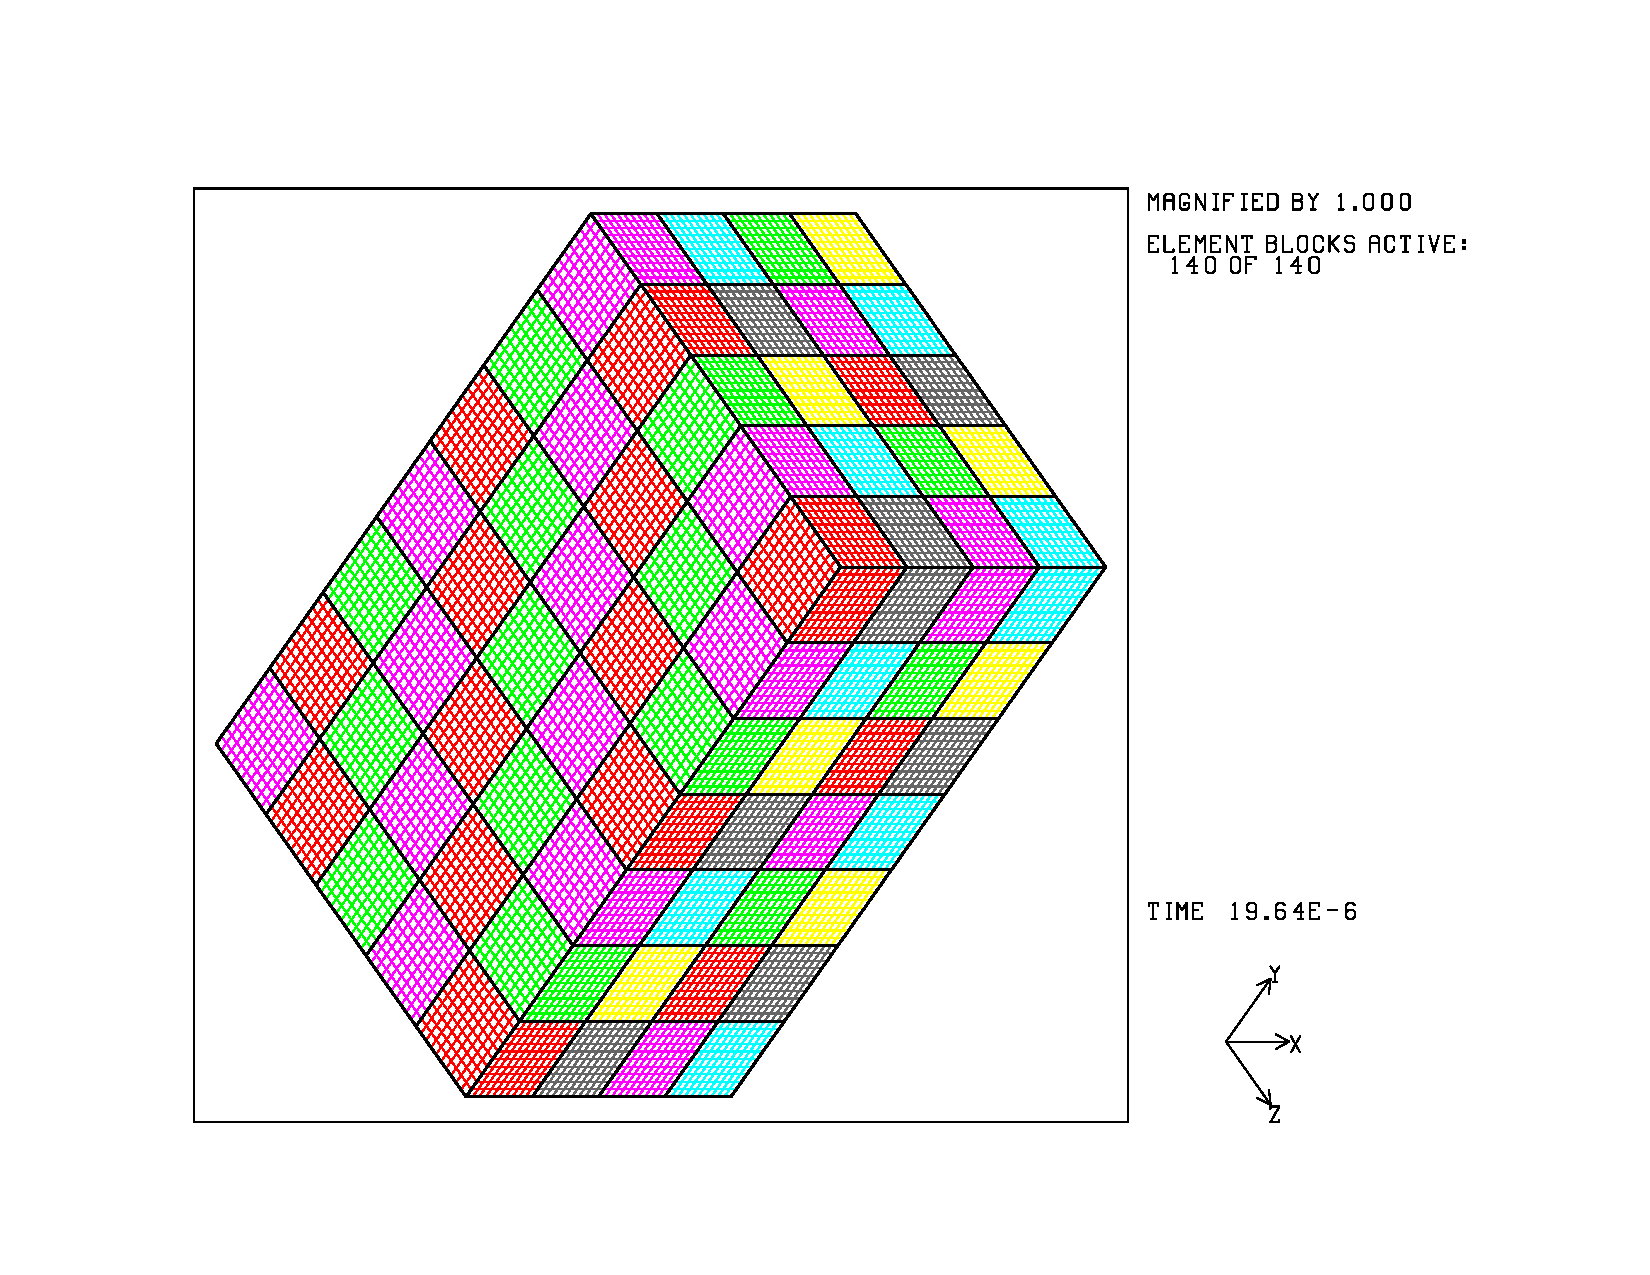
\includegraphics[width=3.25in]{figures/rect_inline}
  \end{minipage}
  \caption{Definition of a three-dimensional \texttt{RECTILINEAR} mesh.}
  \label{fig:rect_inline}
\end{figure}

\clearpage
\subsubsection{Spherical}
\index{Spherical}
{\ttfamily \begin{verbatim}
SPHERICAL
   [subkeyword-list]
END
\end{verbatim}
}

The \texttt{SPHERICAL -- END} block pair allows the description of a
curvilinear spherical mesh centered at the origin and described by an
inner and outer radius, and the extent of revolution in $\theta$ and $\phi$
directions.  Angle $\theta$ is measured counter-clockwise about the z-axis from
the x-axis, and angle $\phi$ is measured counter-clockwise from the y-axis
about the x-axis.  The number of elements and blocks in each
curvilinear coordinate direction are specified by the keywords in
Table~\ref{tab:inlinemesh-radial}.  The parameters \texttt{PHI, NPHI,
and BPHI} are only appropriate for 3D problems. When used in 2D
simulations, \texttt{CYLINDRICAL} and \texttt{SPHERICAL} keywords
produce identical meshes.

\threecolumntable{
  Keywords for \texttt{SPHERICAL -- END}.
  \label{tab:inlinemesh-radial}
}{
\hline
  Sub-Keyword & Input & Description \\

\hline \hline
  \texttt{NR} & \texttt{int} &
       Number of cells in r-direction. \\ \hline
  \texttt{NTHETA} & \texttt{int} &
       Number of cells in $\theta$-direction. \\ \hline
  \texttt{NPHI} & \texttt{int} &
       Number of cells in $\phi$-direction. \\ \hline
  \texttt{BR} & \texttt{int} &
       Number of blocks in the r-direction. \\ \hline
  \texttt{BTHETA} & \texttt{int} &
       Number of blocks in $\theta$-direction. \\ \hline
  \texttt{BPHI} & \texttt{int} &
       Number of blocks in $\phi$-direction. \\ \hline
  \texttt{RI} & \texttt{real} &
       Inner radius \\ \hline
  \texttt{RO} & \texttt{real} &
       Outer radius \\ \hline
  \texttt{THETA} & \texttt{real} &
       Angular extent in $\theta$ (degrees,0.-180. in 3D, 0.-360. in 2D) \\ \hline
  \texttt{PHI} & \texttt{real} &
       Angular extent in $\phi$ (0.-360) \\ \hline
}

%\clearpage

An example of a mesh definition syntax with the
\texttt{SPHERICAL} option is illustrated in
Figure~\ref{fig:test_radial} for a 2D simulation.  An example of 3D
spherical mesh generation follows in
Figure~\ref{fig:str_inline_sphere}.

\begin{figure}[htb]
  \centering
  \begin{minipage}[c]{0.4\linewidth}
    \centering
{\ttfamily \begin{verbatim}
mesh
  spherical
    ri = 0.0
    ro = 0.5
    theta = 45
    ntheta = 10
    nr = 20
    br = 2
    btheta = 2
  end
end
\end{verbatim}}
  \end{minipage}%
  \hfil
  \begin{minipage}[c]{0.6\linewidth}
    \centering
      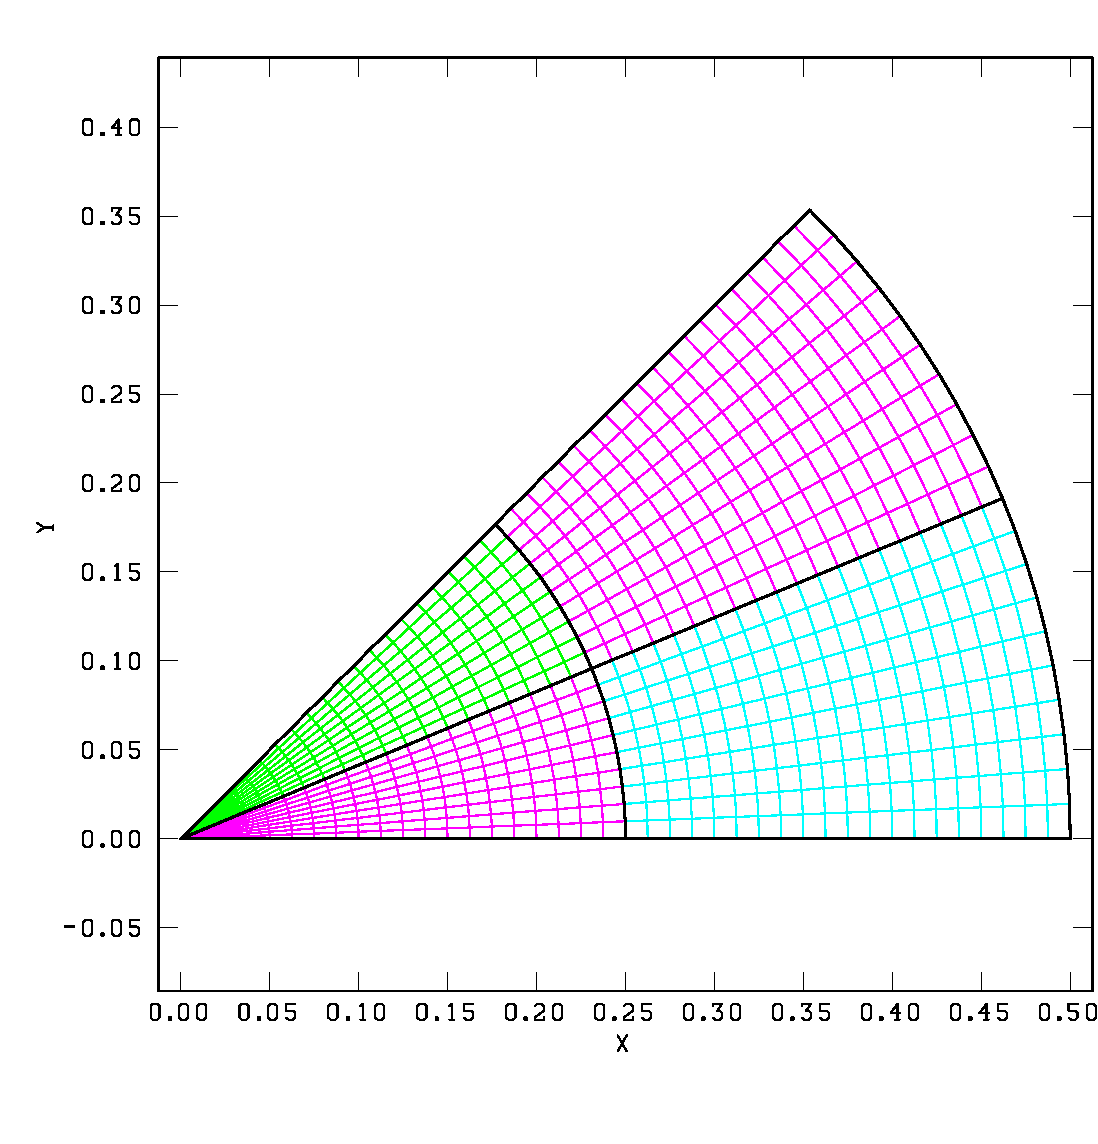
\includegraphics[width=2.75in]{figures/test_radial}
  \end{minipage}
  \caption{Definition of a two-dimensional spherical mesh.}
  \label{fig:test_radial}
\end{figure}

%\clearpage

\begin{figure}[htb]
\centering
  \begin{minipage}[c]{0.4\linewidth}
    \centering
{\ttfamily \begin{verbatim}
mesh
  spherical
    ri = 0.5
    ro = 1.0
    theta = 180.0
    ntheta = 10
    nr = 10
    br = 2
    btheta = 2
    bphi = 2
    nphi = 10
    phi = 90
  end
end
\end{verbatim}}
  \end{minipage}%
  \hfil
  \begin{minipage}[c]{0.6\linewidth}
    \centering
      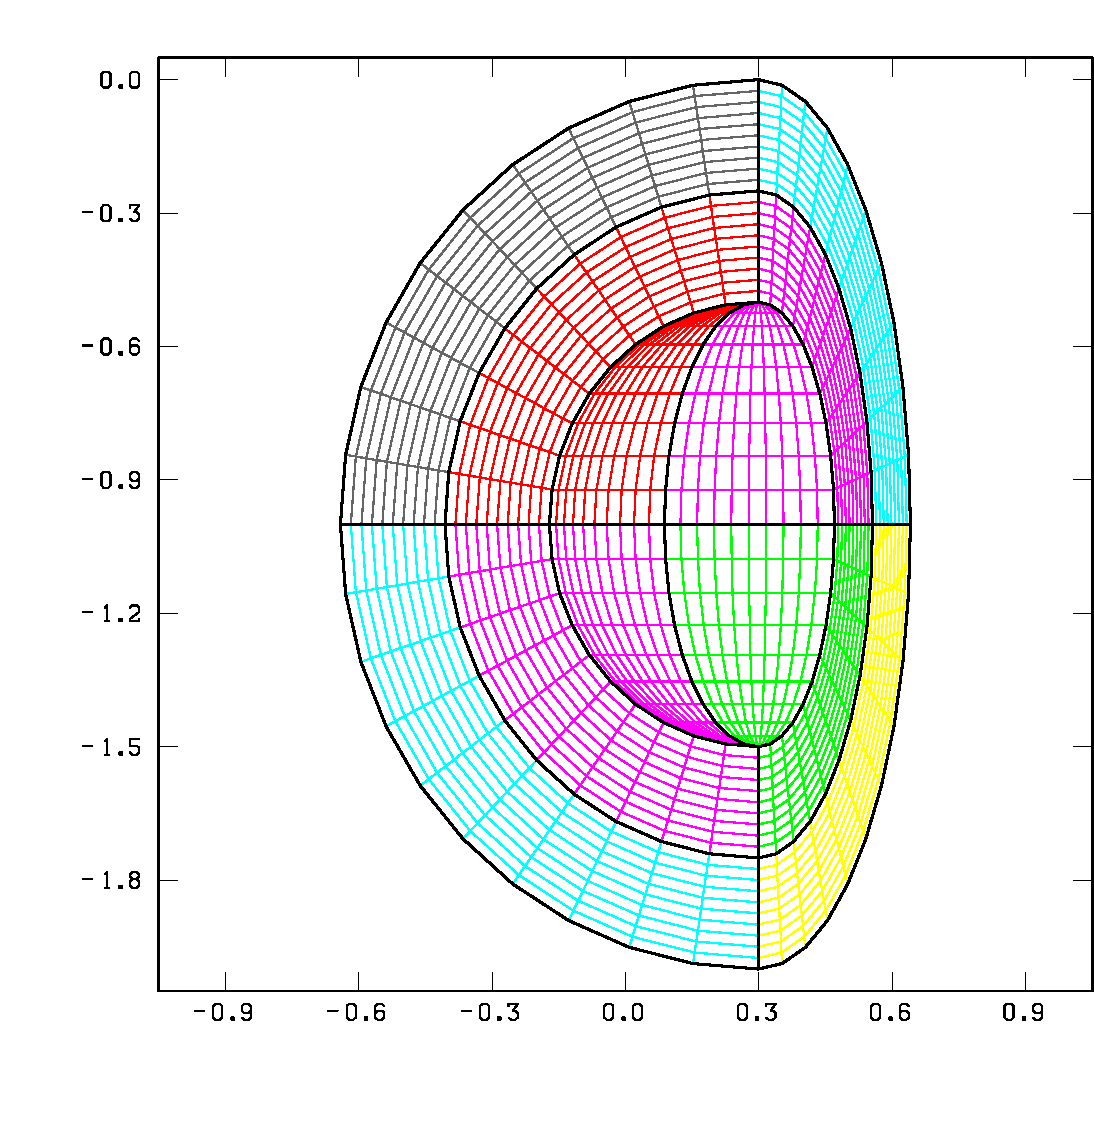
\includegraphics[width=2.75in]{figures/str_inline_sphere}
  \end{minipage}
  \caption{Definition of a three-dimensional spherical mesh.}
  \label{fig:str_inline_sphere}
\end{figure}

\clearpage
\subsubsection{Cylindrical}
\index{Cylindrical}
{\ttfamily \begin{verbatim}
CYLINDRICAL
   [subkeyword-list]
END
\end{verbatim}
}

The \texttt{CYLINDRICAL -- END} block pair allows the description of a
curvilinear cylindrical mesh centered at the origin in x and y, and
aligned along the z-axis.  It is described by an inner and outer
radius, the extent of revolution in angle $\theta$ about the z-axis,
and its start and end in the z-direction.  Angle $\theta$ is measured
counter-clockwise about the z-axis from the x-axis.  The number of
elements and blocks in each indicial direction are specified by the
keywords in Table~\ref{tab:inlinemesh-cylinder}.  The parameters
\texttt{ZMIN, ZMAX, NZ, and BZ} are only appropriate for 3D
problems.  When used in 2D solutions, \texttt{CYLINDRICAL} and
\texttt{SPHERICAL} produce identical meshes.

\threecolumntable{
  Keywords for \texttt{CYLINDRICAL -- END}.
  \label{tab:inlinemesh-cylinder}
}{
\hline
  Sub-Keyword & Input & Description \\

\hline \hline
  \texttt{NR} & \texttt{int} &
       Number of cells in r-direction. \\ \hline
  \texttt{NTHETA} & \texttt{int} &
       Number of cells in $\theta$-direction. \\ \hline
  \texttt{NZ} & \texttt{int} &
       Number of cells in z-direction. \\ \hline
  \texttt{BR} & \texttt{int} &
       Number of blocks in the r-direction. \\ \hline
  \texttt{BTHETA} & \texttt{int} &
       Number of blocks in $\theta$-direction. \\ \hline
  \texttt{BZ} & \texttt{int} &
       Number of blocks in z-direction. \\ \hline
  \texttt{RI} & \texttt{real} &
       Inner radius \\ \hline
  \texttt{RO} & \texttt{real} &
       Outer radius \\ \hline
  \texttt{THETA} & \texttt{real} &
       Angular extent in $\theta$ degrees, 0.-360. \\ \hline
  \texttt{ZMIN} & \texttt{real} &
       Start of mesh in z-direction \\ \hline
  \texttt{ZMAX} & \texttt{real} &
       End of mesh in z-direction \\ \hline
}

An example of a \textsc{pamgen} mesh definition with the
\texttt{CYLINDRICAL} option is illustrated in
Figure~\ref{fig:rect_cylinder}.

\begin{figure}[htbp]
\centering
  \begin{minipage}[c]{0.4\linewidth}
    \centering
{\ttfamily \begin{verbatim}
mesh
  cylindrical
    ri = 0.5
    ro = 1.0
    theta = 90.0
    ntheta = 10
    nr = 10
    br = 2
    zmin = 1.0
    zmax = 2.0
    nz = 10
    bz = 2
  end
end
\end{verbatim}}
  \end{minipage}%
  \hfil
  \begin{minipage}[c]{0.6\linewidth}
    \centering
      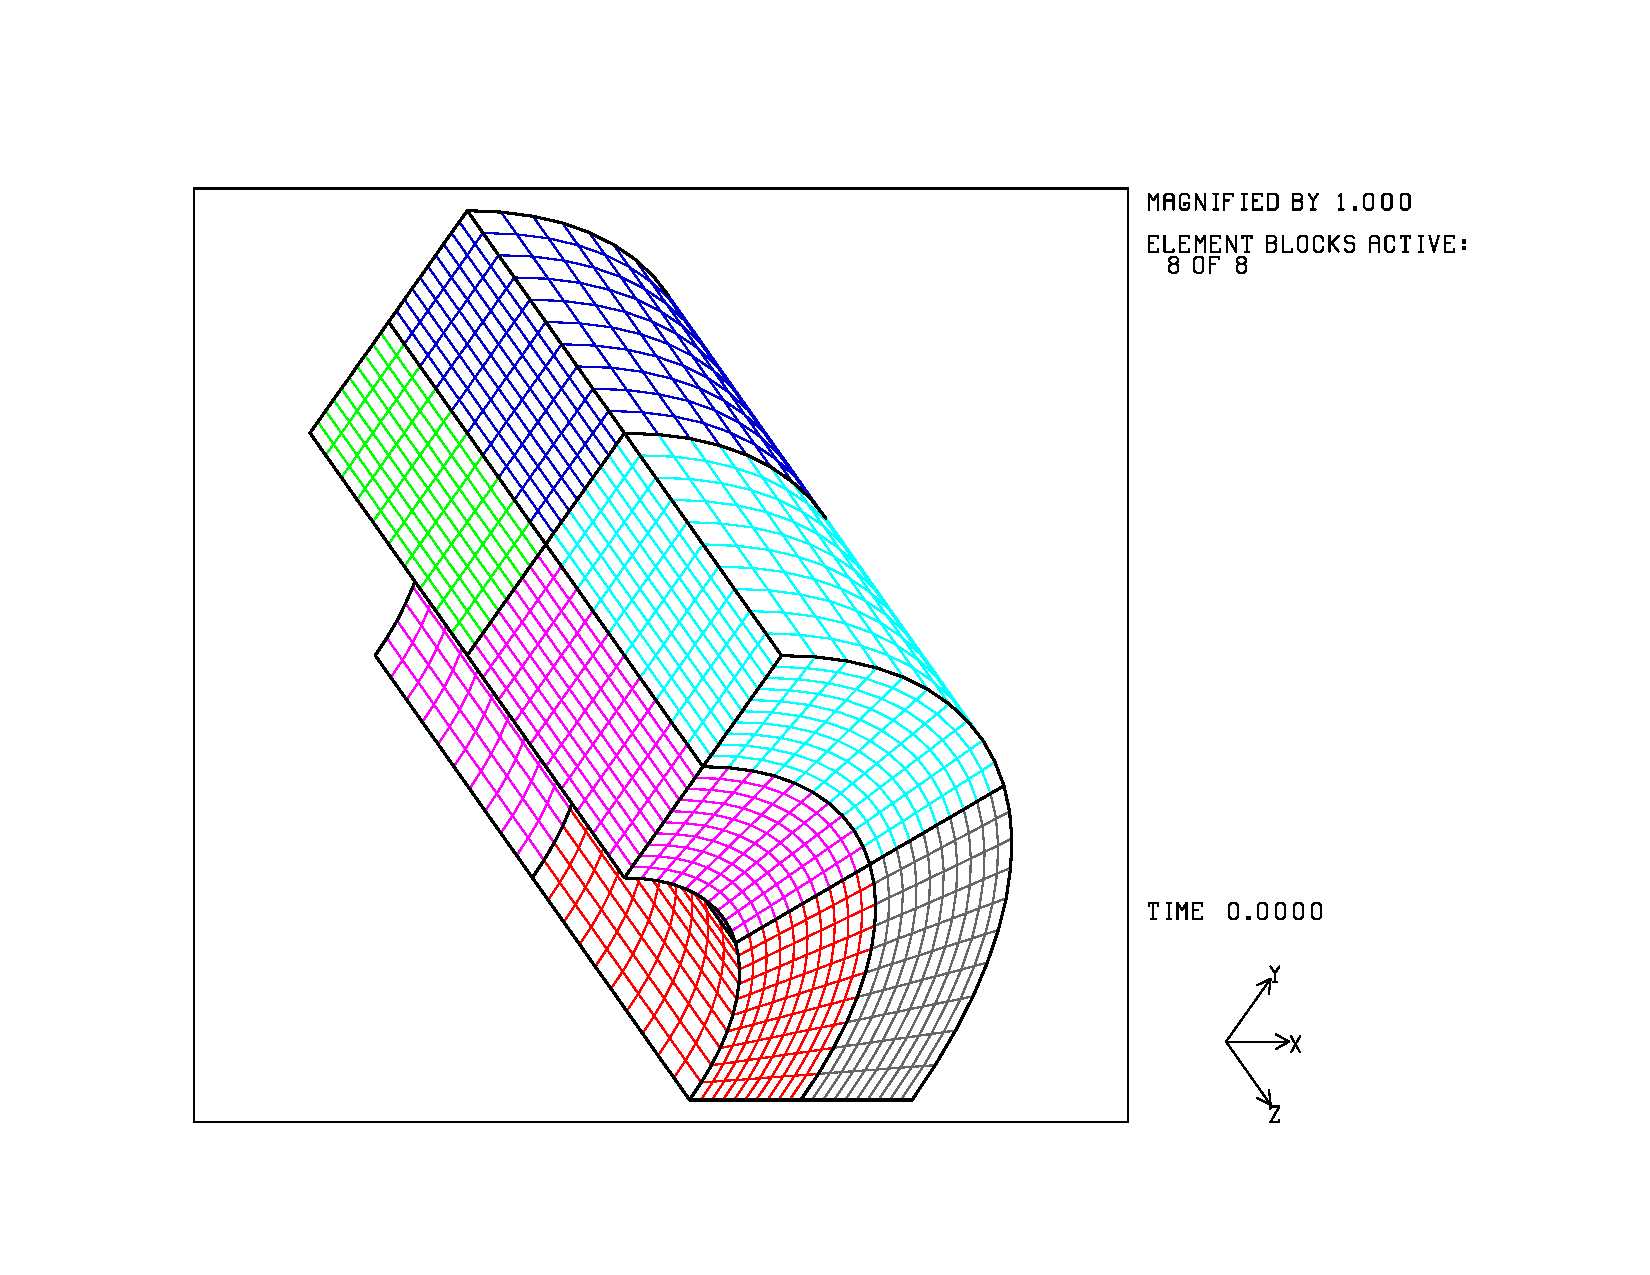
\includegraphics[width=3.5in]{figures/cylinder}
  \end{minipage}
  \caption{Three dimensional \texttt{CYLINDRICAL} mesh.}
  \label{fig:rect_cylinder}
\end{figure}

\clearpage
\subsubsection {Radial and Radial Trisection}
\index{Radial}
\index{Radial Trisection}
\index{Trisection}
{\ttfamily \begin{verbatim}
{RADIAL | RADIAL TRISECTION }
   [ENFORCE PERIODICITY]
   [TRISECTION BLOCKS, int]
   [TRANSITION RADIUS, int]
   [ZMIN real]
   NUMZ int
     ZBLOCK int real {INTERVAL int | FIRST SIZE real [LAST SIZE real]}
   {NUMR | NUMX} int INITIAL RADIUS real
     RBLOCK int real {INTERVAL int | FIRST SIZE real [LAST SIZE real]}
   {NUMA | NUMY} int
     ABLOCK int real {INTERVAL int | FIRST SIZE real [LAST SIZE real]}
END
\end{verbatim}
}

The \texttt{RADIAL} and \texttt{RADIAL TRISECTION} block pairs allow the description of
a
curvilinear cylindrical mesh centered at the origin in x and y, and
aligned along the z-axis.  The \texttt{RADIAL TRISECTION -- END}
block pair fills in the center of the cylindrical mesh with transition
elements.  These options are similar to the \texttt{CYLINDRICAL}
but they have a different set of controls on element distribution.  The
successful creation of these meshes requires sequential
specification of the information for the number of elements blocks and
their sizes in each coordinate direction.

The \texttt{ENFORCE PERIODICITY} keyword applies only to \texttt{RADIAL} and \texttt{RADIAL TRISECTION} mesh descriptions that meet certain requirements:
\begin{itemize}
  	\item The meshes must have azimuthal angles of 90, 180, or 360 degrees.
	\item The meshes must have a single block of elements in the azimuthal direction.
	\item The meshes must have an even number of elements in each 90 degree segment of the mesh.
	\item For \texttt{RADIAL TRISECTION} meshes, one transition zone is required for each 90 degrees of azimuth.
\end{itemize}

This keyword causes the mesh generation to perform all node coordinate calculations in the first 45 degrees of the azimuthal domain. Coordinate locations of nodes ouside of 45 degrees are formed by permuting the sign and oder of the components of periodically corresponding nodes' locations. This guarantees that there will be no differences between the absolute floating point values of periodically corresponding nodes' coordinates.

The \texttt{NUMZ | NUMR | NUMA} keywords are followed by an integer
specifying the number
of element blocks in that coordinate direction. The
\texttt{NUMR} line includes an additional real parameter that
specifies the inner radius of the cylindrical mesh. Specification of
an inner radius of 0.0 will result in degenerate elements with
co-located nodes along the \texttt{Z} axis. The innner radius
specification is ignored for \texttt{RADIAL TRISECTION} meshes.

Immediately following
the \texttt{NUMZ int | NUMR int INITIAL RADIUS real | NUMA int} lines, there must be a \texttt{ZBLOCK |
  RBLOCK | ABLOCK} line for each of the blocks in that direction.
These lines specify the spatial extent of the particular block and the
distribution of elements in the block in that direction. The \texttt{INTERVAL int} keyword
specifies a fixed number of elements in the
block. A \texttt{FIRST SIZE real LAST SIZE real} pair specifies the absolute
size of the first and last elements in the block. When the \texttt{FIRST SIZE real LAST SIZE real} specification is
used, the element sizing will be linear between the first and last
elements. The sizes of the first and last elements may be
adjusted slightly to provide linear sizing. The approximate number of elements that will be generated using \texttt{FIRST SIZE} and \texttt{LAST SIZE} sizing controls is given by truncating to an integer, the length of the mesh segment divided by the average of the \texttt{FIRST SIZE} and \texttt {LAST SIZE} values. There is a slight chance that this calculation will result in a different number of elements on different computer platforms.  Omission of the
\texttt{LAST real} keyword is equivalent to setting the element size
to that given by the \texttt{FIRST SIZE real} keyword.

The \texttt{RADIAL TRISECTION -- END} block pair requires the
additional input of \texttt{TRISECTION BLOCKS, int} and it accepts the
optional \texttt{TRANSITION RADIUS, real} keyword value pair.  The
\texttt{TRISECTION BLOCKS} keyword specifies the number of transition
zones that will be used in the central region of the mesh. This
number must be supplied. One transition zone is recommended for each
90 degrees of azimuth.  The \texttt{TRANSITION RADIUS} is the distance
from the origin to the corners of the transition zones of
mesh. Without this parameter the transition radius is chosen to be one
half of the radial thickness of the first block.  When \texttt{RADIAL TRISECTION} is selected, any \texttt{INITIAL RADIUS} supplied is
  ignored.

The \texttt{ZMIN real} keyword value pair is available to specify an offset for the
entire mesh in the \texttt{Z} direction.

If the cumulative values of the sizes of the azimuthal blocks, given
by the second argument of \texttt{ABLOCK int real} is equal to 360.0 degrees, then the mesh
will form an single closed ring of elements.


An example of \textsc{pamgen} mesh definition with the
\texttt{RADIAL} option is illustrated in
Figure~\ref{fig:rect_cubit_radial}.

\begin{figure}[!thbp]
\centering
\hfil
  \begin{minipage}[c]{1.0\linewidth}
    \centering
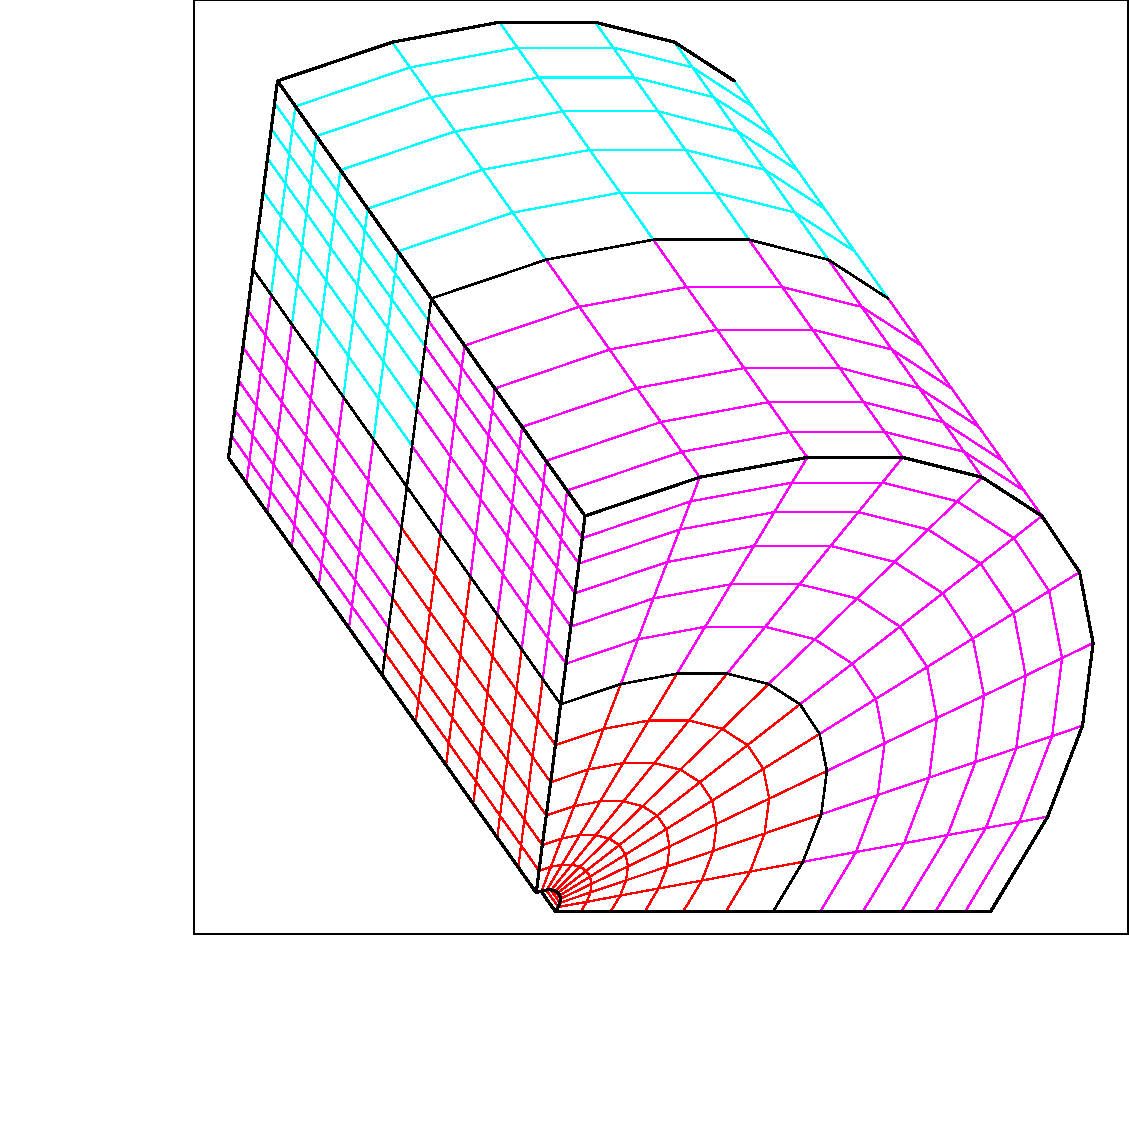
\includegraphics[width=3.0in]{figures/cubit_radial1}
{\ttfamily \begin{verbatim}
mesh
  radial
    numz 2
      zblock 1 10.0 first size 1 last size 2
      zblock 2 10.0 first size 2 last size 1
    numr 2 initial radius 1.
      rblock 1 10. first size 1. last size 2.
      rblock 2 10. first size 2. last size 1.
    numa 1
      ablock 1 120. interval 10
  end
end
\end{verbatim}}
  \end{minipage}%
  \caption{Three dimensional \texttt{RADIAL} mesh.}
  \label{fig:rect_cubit_radial}
\end{figure}



A second example of \textsc{pamgen} mesh definition with the
\texttt{RADIAL} option is illustrated in
Figure~\ref{fig:rect_cubit_radial2}. In this case the sum of the
azimuthal blocks is 360.0 and the mesh is a
complete cylinder.

\begin{figure}[htbp]
\centering
  \begin{minipage}[c]{0.4\linewidth}
    \centering
{\ttfamily \begin{verbatim}
mesh
  radial
  numz 1
    zblock 1 10.0 interval 6
  numr 3
    rblock 1 2. interval 12
    rblock 2 5. interval 6
    rblock 3 5. interval 12
  numa 1
    ablock 1 360. interval 36
 end
end
\end{verbatim}}
  \end{minipage}%
  \hfil
  \begin{minipage}[c]{0.6\linewidth}
    \centering
      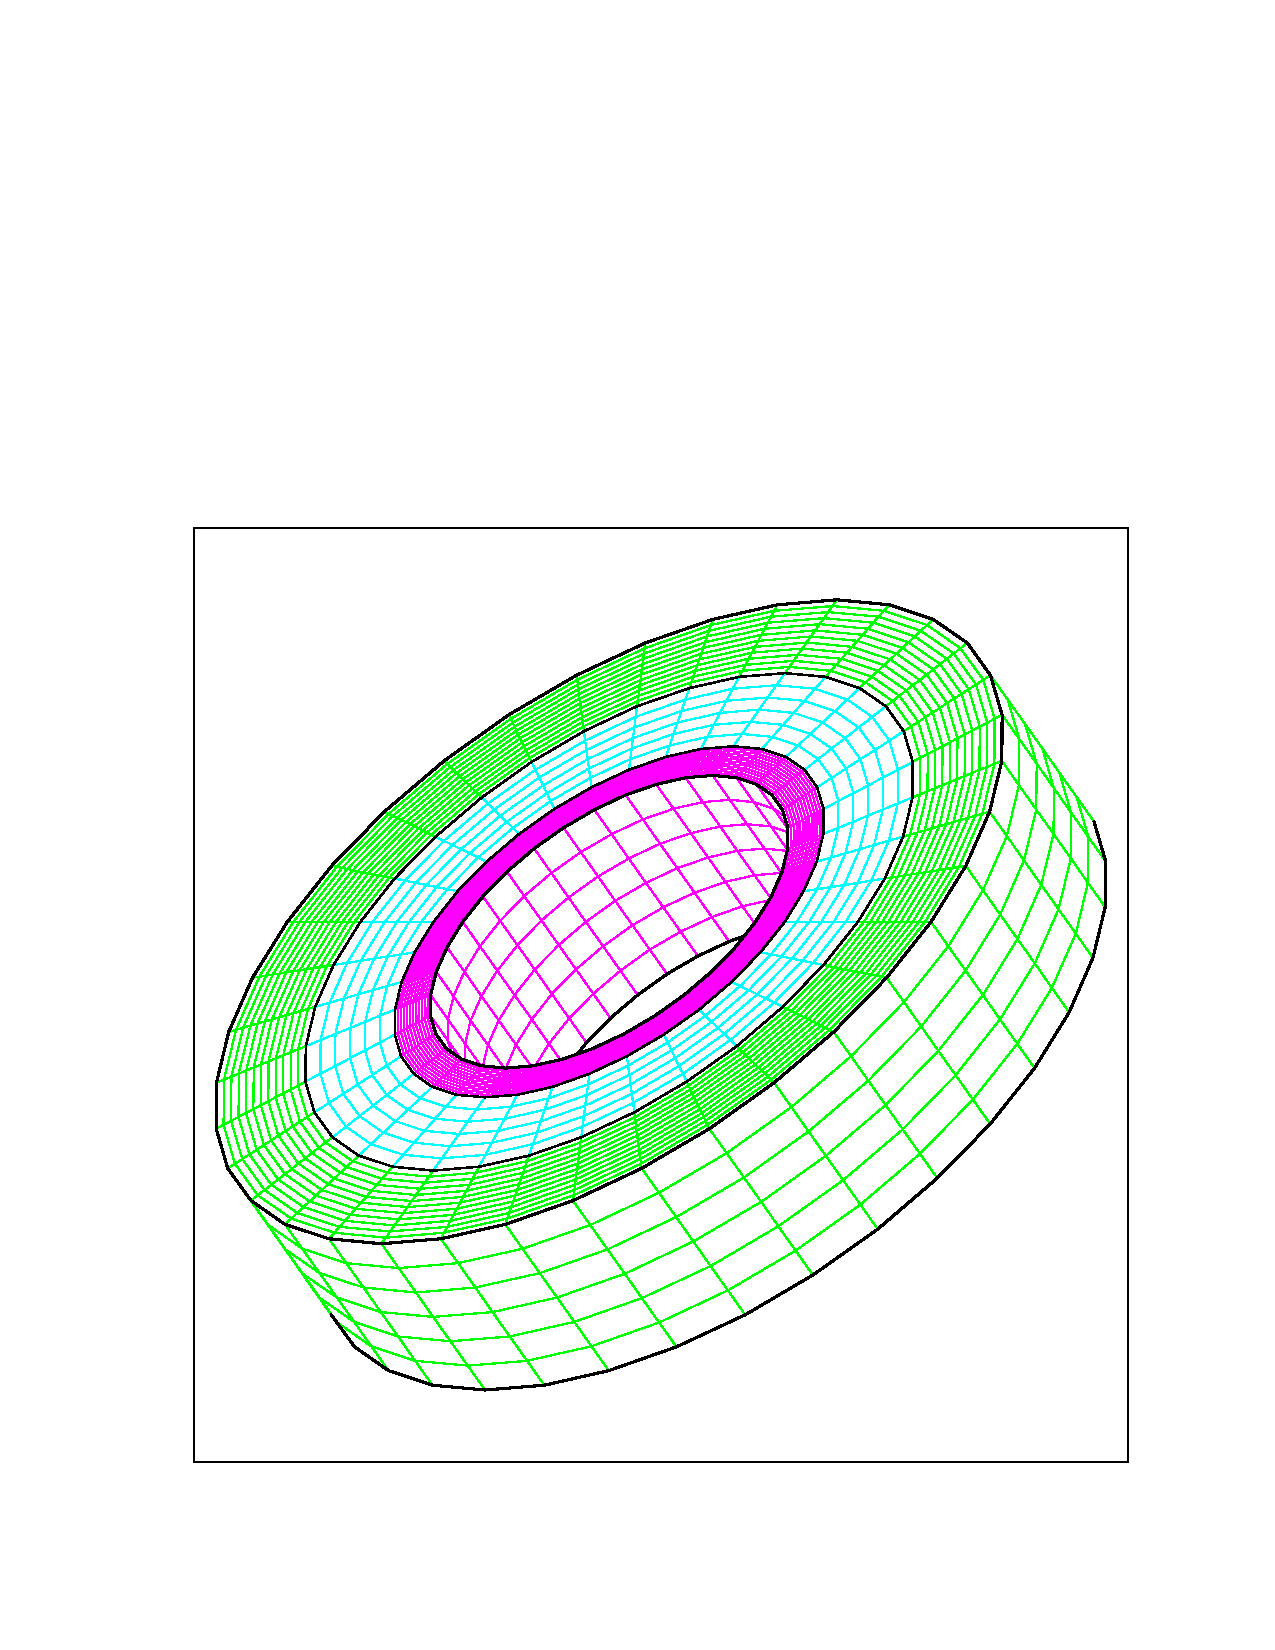
\includegraphics[width=3.0in]{figures/cubit_radial2}
  \end{minipage}
  \caption [A 360 degree \texttt{RADIAL} mesh.]{Three dimensional \texttt{RADIAL} mesh with azimuthal
    angle of 360 degrees.}
  \label{fig:rect_cubit_radial2}
\end{figure}

An example of a \textsc{pamgen} mesh definition with the
\texttt{RADIAL TRISECTION} option is illustrated in
Figure~\ref{fig:cubit_radial_trisect3}. This figure is annotated to
show the correspondence between input parameters and the
resulting mesh. This mesh uses a \texttt{TRISECTION BLOCKS} setting of 3. In this case the azimuthal
angle is 90. degrees and the \texttt{FIRST SIZE}, \texttt{LAST SIZE},
 and \texttt{TRANSITION RADIUS} directives are used.

\begin{figure}[!thbp]
\centering
  \hfil
  \begin{minipage}[c]{1.0\linewidth}
    \centering
      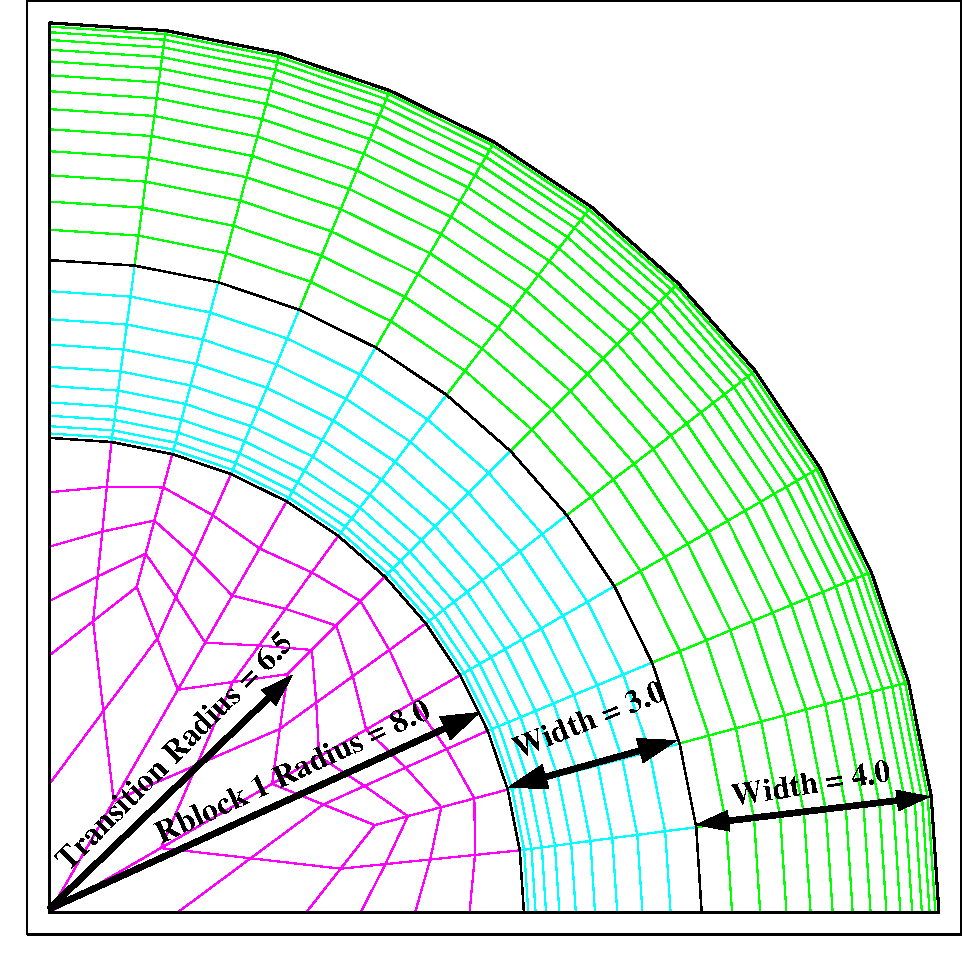
\includegraphics[width=5.5in,height=4.5in]{figures/cubit_tris_rad_grad_trans}
{\ttfamily \begin{verbatim}
mesh
  radial trisection
    trisection blocks, 3
    transition radius, 6.5
    numz 1
      zblock 1 1. interval 1
    numr 3
      rblock 1 8.0 interval 4
      rblock 2 3.0 first size 0.05 last size 0.5
      rblock 3 4.0 first size 0.5 last size 0.05
    numa 1
      ablock 1 90. interval 12
  end
end
\end{verbatim}}
  \end{minipage}
  \caption [A \texttt{RADIAL TRISECTION} mesh with three trisection blocks.]{A \texttt{RADIAL TRISECTION} mesh with azimuthal
    angle of 90 degrees and three trisection blocks. \texttt{FIRST
      SIZE} and \texttt{LAST SIZE} commands are used to specify
    element density.}
  \label{fig:cubit_radial_trisect3}
\end{figure}

An second example of a \textsc{pamgen} mesh definition with the
\texttt{RADIAL TRISECTION} option is illustrated in
Figure~\ref{fig:cubit_radial_trisect1}.

\begin{figure}[htbp]
\centering
  \begin{minipage}[c]{0.4\linewidth}
    \centering
{\ttfamily \begin{verbatim}
mesh
  radial trisection
    trisection blocks, 2
    zmin -0.00075
    numz 1
      zblock 1 1. interval 4
    numr 3
      rblock 1 2.0 interval 4
      rblock 2 3.0 interval 4
      rblock 3 4.0 interval 4
    numa 1
      ablock 1 90. interval 12
  end
end
\end{verbatim}}
  \end{minipage}%
  \hfil
  \begin{minipage}[c]{0.6\linewidth}
    \centering
      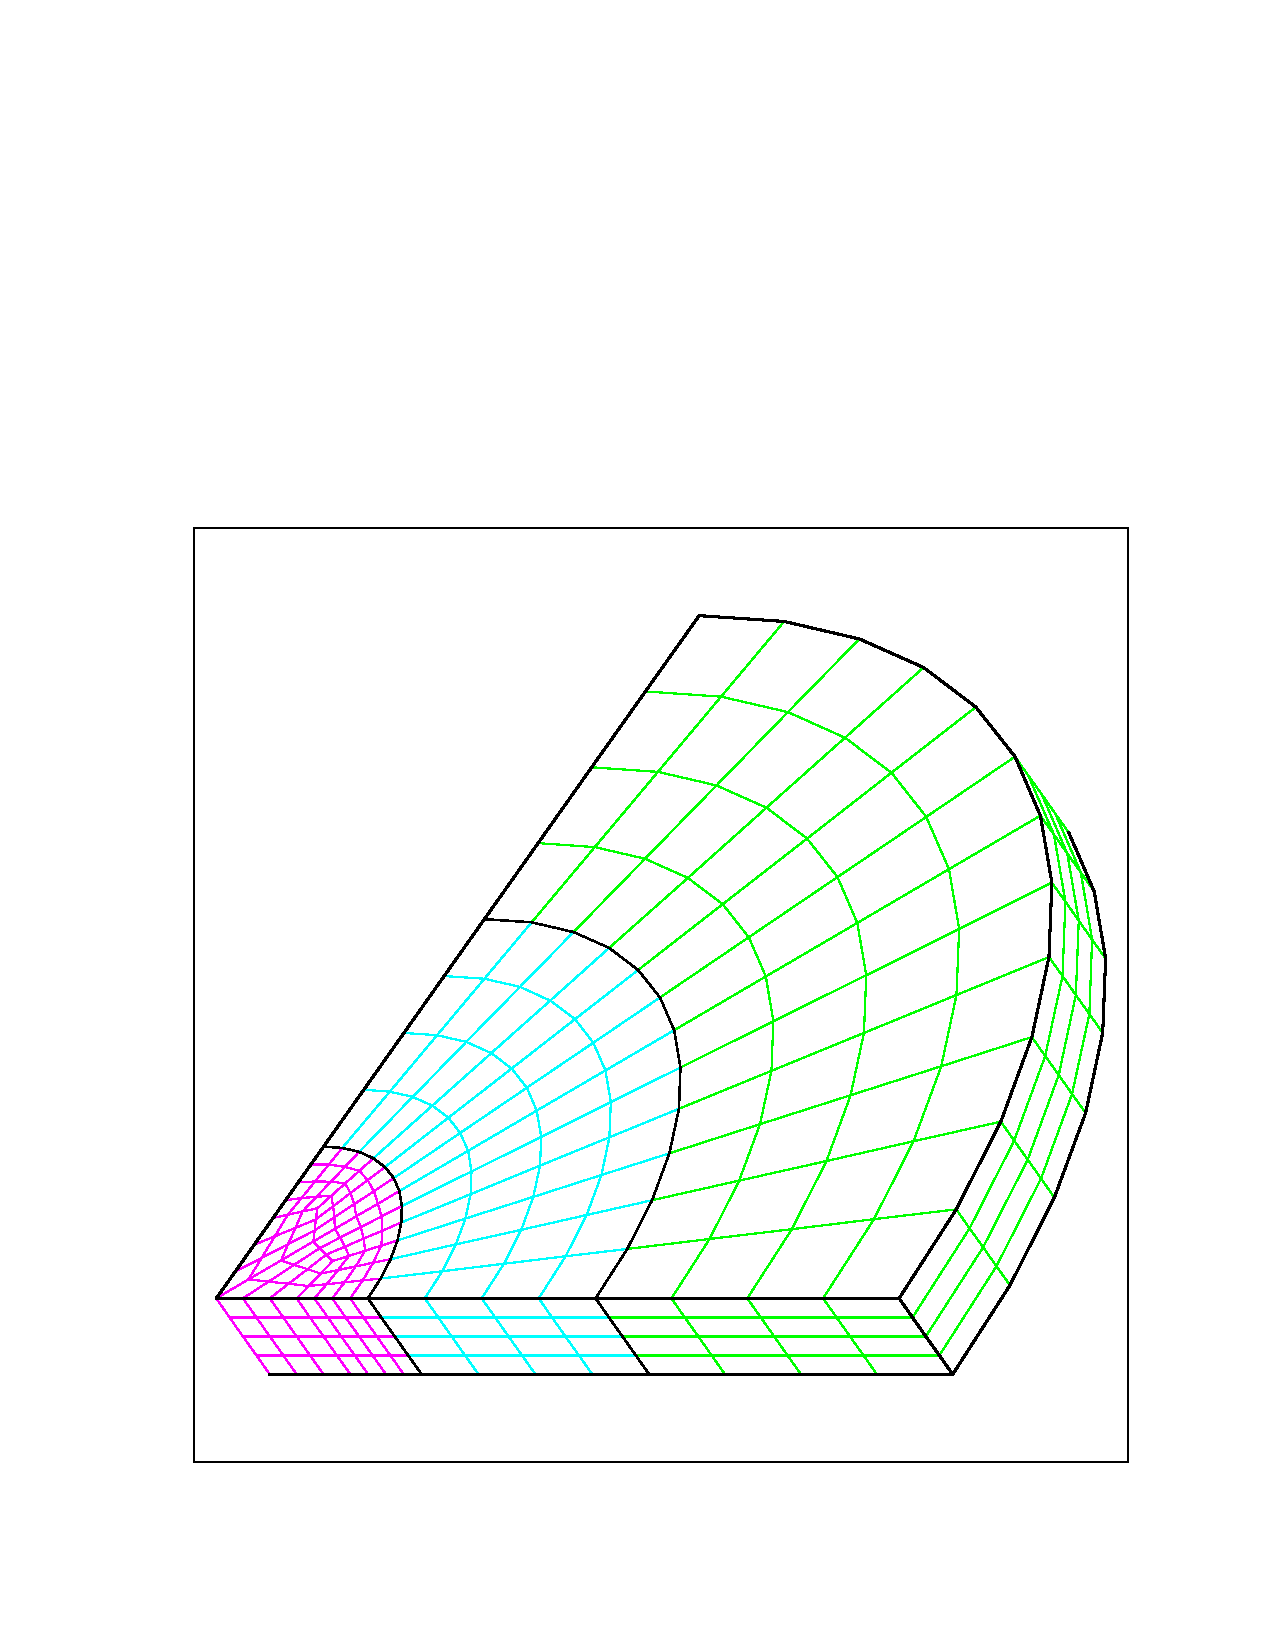
\includegraphics[width=3.0in]{figures/cubit_radial_trisection}
  \end{minipage}
  \caption [A \texttt{RADIAL TRISECTION} mesh with three trisection blocks.] {Three dimensional \texttt{RADIAL TRISECTION} mesh with azimuthal
    angle of 90 degrees and two trisection blocks.}
  \label{fig:cubit_radial_trisect1}
\end{figure}


A third example of a \textsc{pamgen} mesh definition with the
\texttt{RADIAL TRISECTION} option is illustrated in
Figure~\ref{fig:cubit_radial_trisect2}. In this case the azimuthal
angle is 360. degrees and the mesh is a complete circular disk.

\begin{figure}[htbp]
\centering
  \begin{minipage}[c]{0.4\linewidth}
    \centering
{\ttfamily \begin{verbatim}
mesh
  radial trisection
    trisection blocks, 4
    zmin -0.00075
    numz 1
      zblock 1 4. interval 4
    numr 3
      rblock 1 2.0 interval 4
      rblock 2 3.0 interval 4
      rblock 3 5.0 interval 4
    numa 1
      ablock 1 360. interval 32
  end
end
\end{verbatim}}
  \end{minipage}%
  \hfil
  \begin{minipage}[c]{0.6\linewidth}
    \centering
      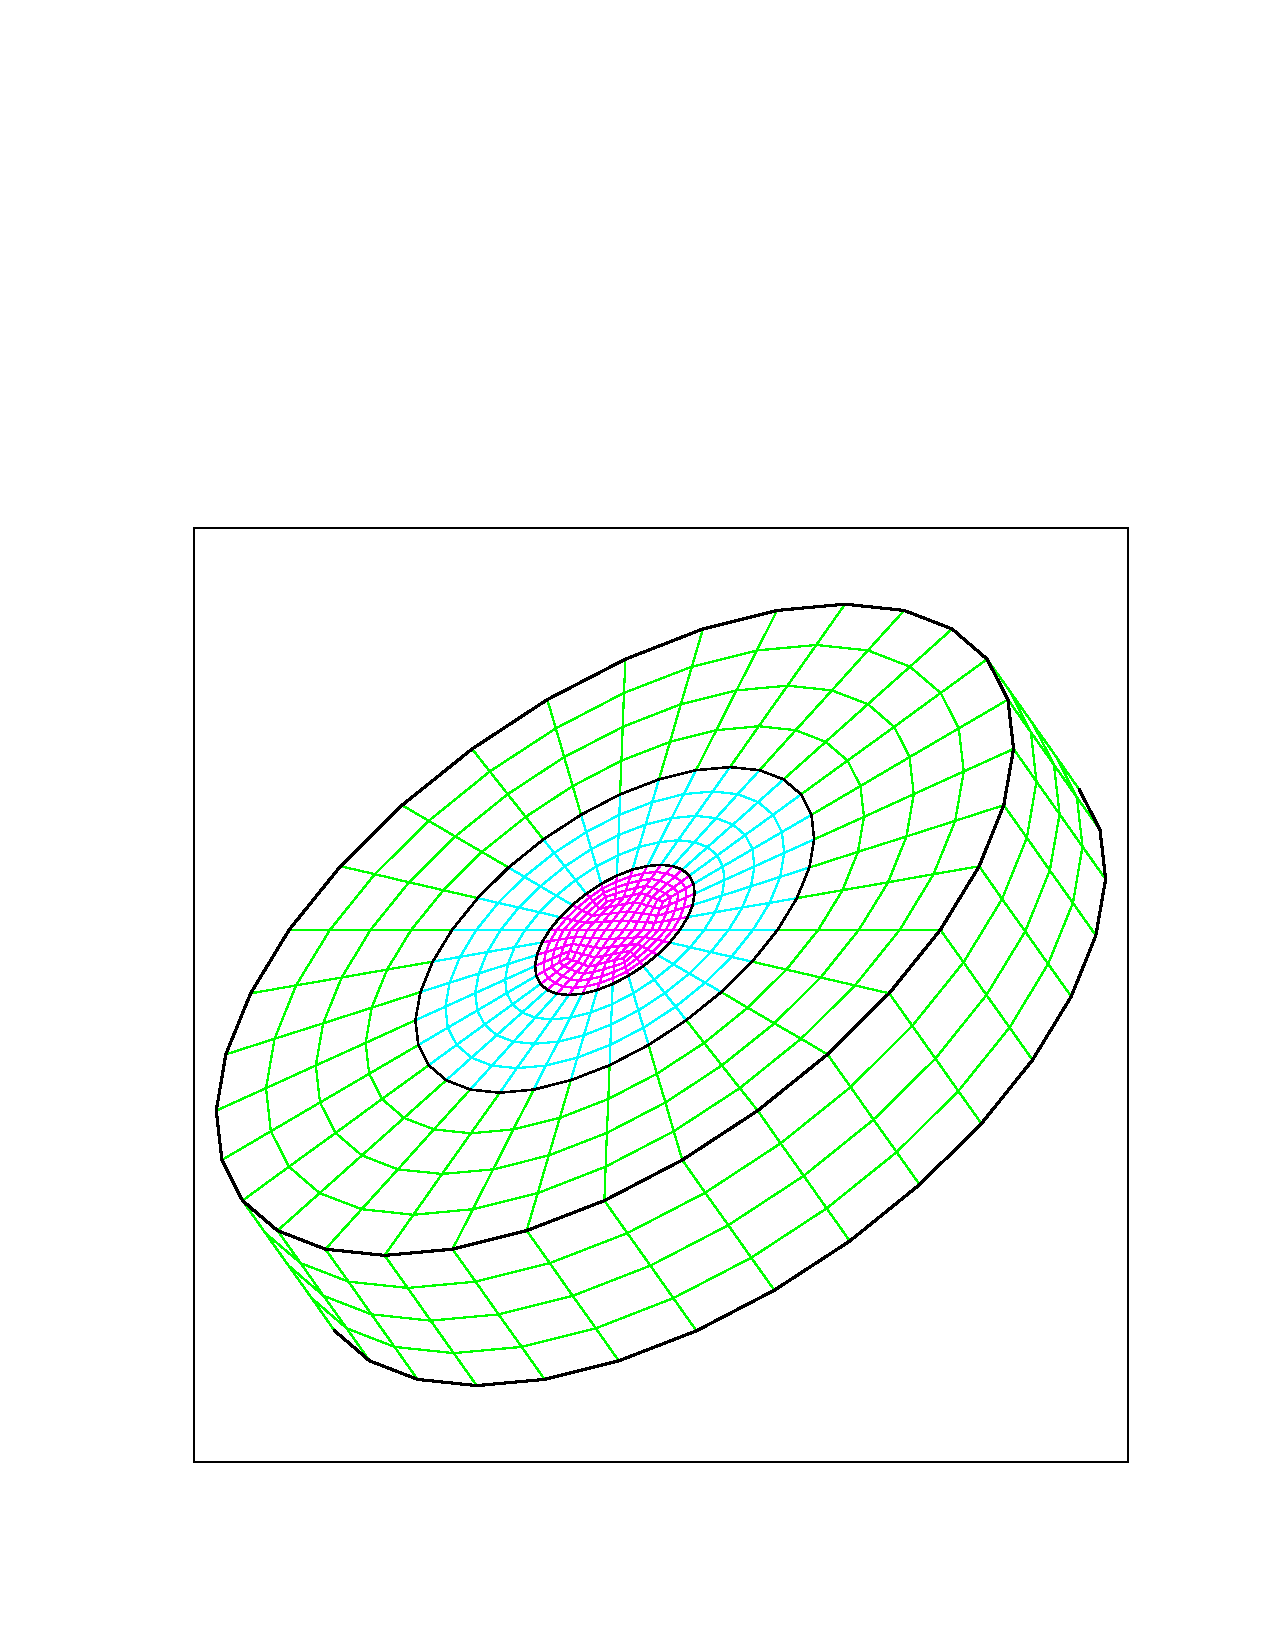
\includegraphics[width=3.0in]{figures/cubit_radial_trisection2}
  \end{minipage}
  \caption [A 360 degree \texttt{RADIAL TRISECTION} mesh.] {Three dimensional \texttt{RADIAL TRISECTION} mesh with azimuthal
    angle of 360 degrees and four trisection blocks.}
  \label{fig:cubit_radial_trisect2}
\end{figure}


\clearpage
\subsubsection {Brick}
\index{Brick}

{\ttfamily \begin{verbatim}
BRICK
  NUMZ int (l)
    ZBLOCK 1 real {INTERVAL int | FIRST SIZE real [LAST SIZE real]}
    ZBLOCK 2 real {INTERVAL int | FIRST SIZE real [LAST SIZE real]}
    ...
    ...
    ZBLOCK l real {INTERVAL int | FIRST SIZE real [LAST SIZE real]}
  NUMX int (m)
    XBLOCK 1 real {INTERVAL int | FIRST SIZE real [LAST SIZE real]}
    XBLOCK 2 real {INTERVAL int | FIRST SIZE real [LAST SIZE real]}
    ...
    ...
    XBLOCK m real {INTERVAL int | FIRST SIZE real [LAST SIZE real]}
  NUMY int (n)
    YBLOCK 1 real {INTERVAL int | FIRST SIZE real [LAST SIZE real]}
    YBLOCK 2 real {INTERVAL int | FIRST SIZE real [LAST SIZE real]}
    ...
    ...
    YBLOCK n real {INTERVAL int | FIRST SIZE real [LAST SIZE real]}
END
\end{verbatim}
}

The \texttt{BRICK} mesh topology type is a more flexible version of the \texttt{RECTILINEAR} type in that it allows different numbers of elements in each element block in each coordinate direction. The creation of a
\texttt{BRICK} mesh is analogous to the \texttt{RADIAL} mesh option
and
successful creation of these meshes requires sequential
specification of the information for the number of elements blocks and
their sizes in each coordinate direction.

The \texttt{NUMX | NUMY | NUMZ} keywords are followed by an integer
specifying the number
of element blocks in that coordinate direction. The

Immediately following
the \texttt{NUMX int | NUMY int | NUMZ int} lines, there must be a \texttt{XBLOCK |
  YBLOCK | ZBLOCK} line for each of the blocks in that direction. The first integer on  this line corresponds to the ordinal (beginning with 1) of the line.
These lines specify the spatial extent of the particular block and the
distribution of elements in the block in that direction. The \texttt{INTERVAL int} keyword
specifies a fixed number of elements in the
block. A \texttt{FIRST SIZE real LAST SIZE real} pair specifies the absolute
size of the first and last elements in the block. When the \texttt{FIRST SIZE real LAST SIZE real} specification is
used, the element sizing will be linear between the first and last
elements. The sizes of the first and last elements may be
adjusted slightly to provide linear sizing. Omission of the
\texttt{LAST real} keyword is equivalent to setting the element size
to that given by the \texttt{FIRST SIZE real} keyword.


An example of a \textsc{pamgen} mesh definition with the
\texttt{BRICK} option is illustrated in
Figure~\ref{fig:brick1}.

\begin{figure}[htbp]
\centering
  \begin{minipage}[c]{0.4\linewidth}
    \centering
{\ttfamily \begin{verbatim}










mesh
  brick
    numz 2
      zblock 1 2. interval 5
      zblock 2 8. interval 4
    numx 2
      xblock 1 5.0 interval 5
      xblock 2 5.0 interval 5
    numy 2
      yblock 1 10. first size 1. last size .1
      yblock 2 10. first size .1 last size 1.
  end
end
\end{verbatim}}
  \end{minipage}%
  \hfil
  \begin{minipage}[c]{0.6\linewidth}
    \centering
      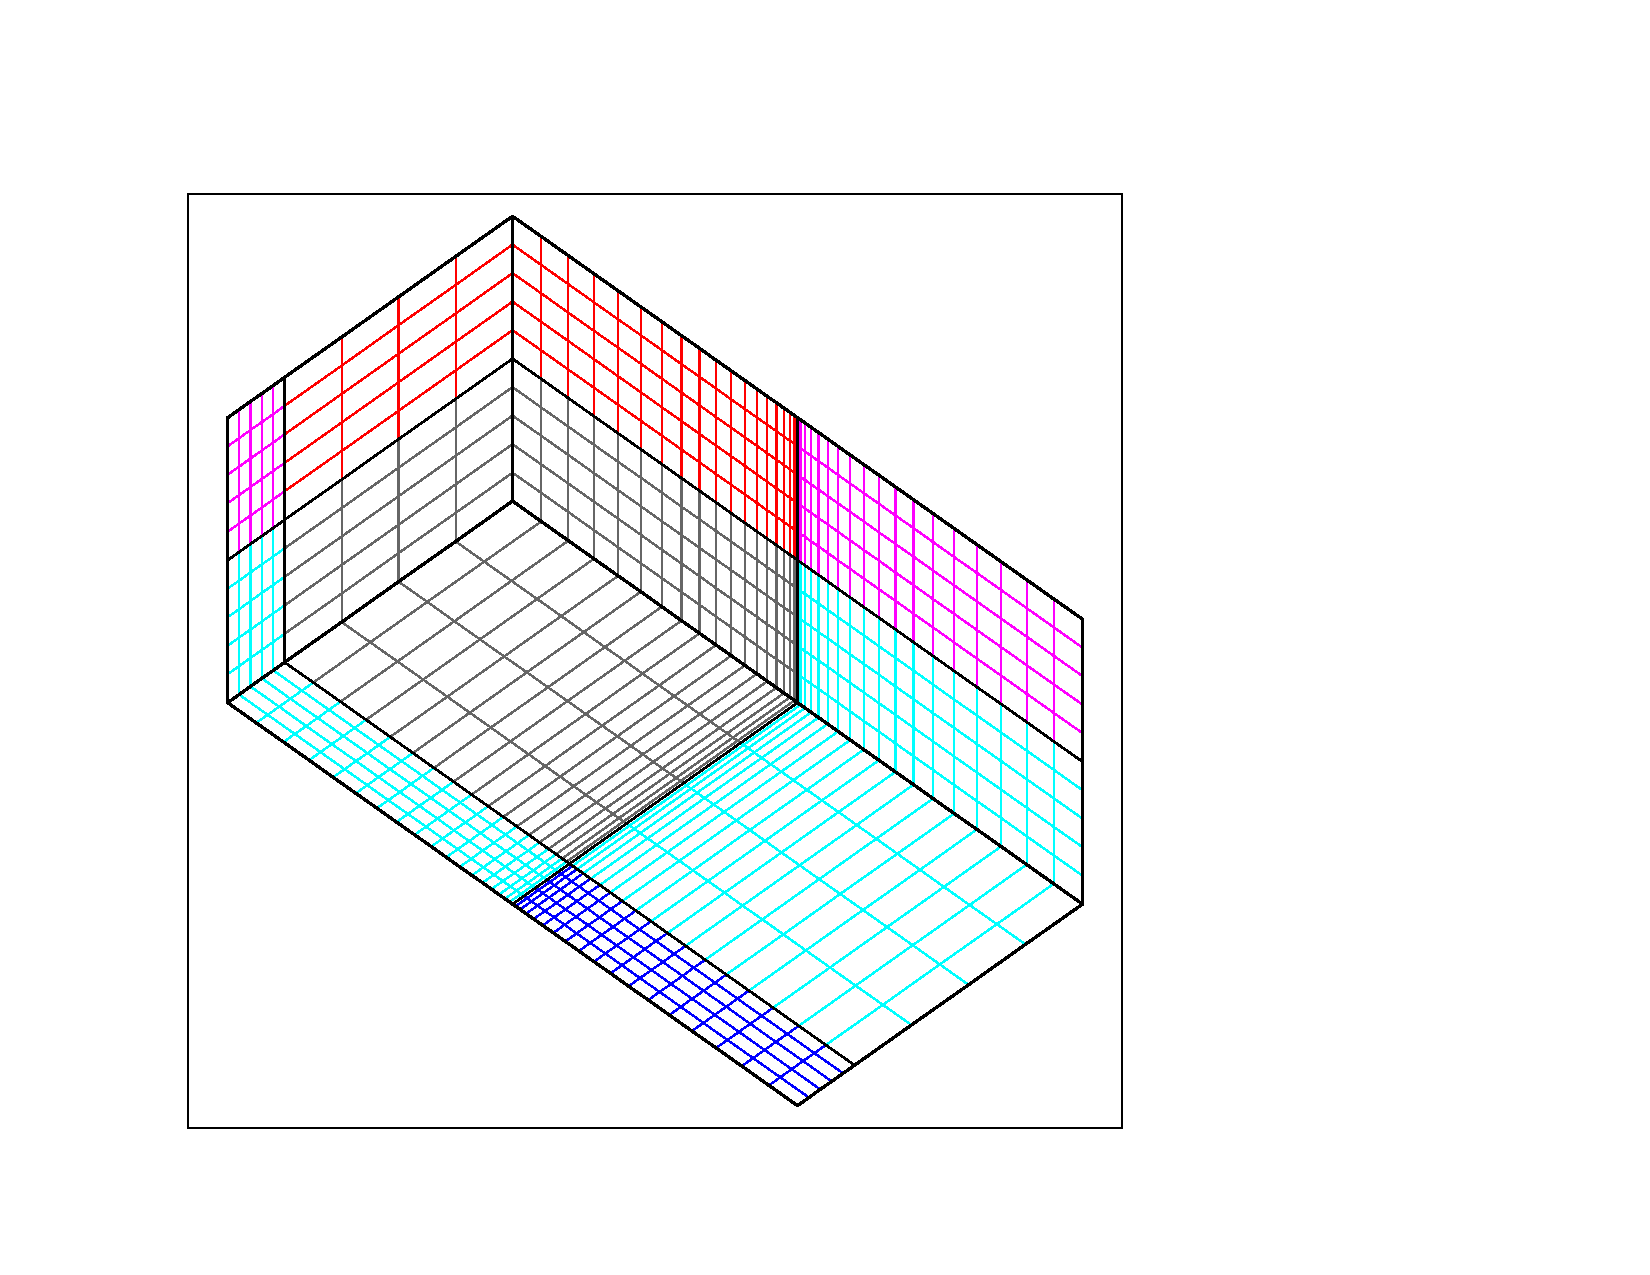
\includegraphics[width=3.0in]{figures/brick}
  \end{minipage}
  \caption{Three dimensional \texttt{BRICK} mesh.}
  \label{fig:brick1}
\end{figure}


\clearpage
\subsection{Boundary Conditions (Nodesets and Sidesets)}
\label{sec:nodesets-sidests}
\index{Boundary Conditions}
\index{Nodesets}
\index{Sidesets}
\index{Set Assign}

{\ttfamily \small \begin{verbatim}
SET ASSIGN
   [{NODESET | SIDESET},{IHI | JHI | ... | V00 | V01 | ... | E00 |
   E01 | ALL| ... }, int]
   [{BLOCK SIDESET | BLOCK NODESET},{IHI | JHI | ... | V00 | V01 |
   ... | E00 | E01 | ... }, int, int]
   ...
END
\end{verbatim}
}

The \texttt{SET ASSIGN -- END} keyword pair allows the specification
of nodesets and sidesets on the exterior of meshes.  These
nodesets and sidesets can be used for specifying boundary conditions
on the domain. The nodeset or sideset is applied to the topological
face, edge, or vertex associated with the prescribed topological
direction. The mesh domain topology and associated labels are
shown in Figure~\ref{fig:set_assign_topology}.This specification
applies to the entire  domain and cannot be used to
specifiy individual blocks.

The most commonly used sub-domains are the exterior faces of the
domain. They can be prescribed using \textsc {IHI, JHI, KHI, ILO,
JLO,} or \textsc {KLO}. For RECTILINEAR meshes \textsc {I,J,} and
\textsc {K} correspond to the coordinate directions x, y, and z. For
SPHERICAL meshes \textsc {I,J,} and \textsc {K} correspond to the
coordinate directions r, $\theta$, and $\phi$. For CYLINDRICAL meshes \textsc
{I,J,} and \textsc {K} correspond to the coordinate directions r,
$\theta$, and z.  The \textsc {KHI, KLO} options do not exist in two
dimension simulations.

The \textsc{ALL} option for nodesets places all the nodes of the mesh in a
nodeset with the requested id. The \textsc{ALL} option is not available for
sidesets.

Specifying a nodeset on the \textsc{ILO} face of a \texttt{RADIAL TRISECTION} mesh
refers to the edge aligned with the Z axis (see Figure~\ref{fig:block_ss}).
Sidesets may not be  specified on the \textsc{ILO} face of
\texttt{RADIAL TRISECTION} meshes.

\begin{figure}[htbp]
{\ttfamily \small \begin{verbatim}
  Side: 0-4-7-3  - ILO      k  7---------6      Edge:  0-1 - E00
  Side: 1-2-6-5  - IHI      | /|  j     /|      Edge:  1-2 - E01
  Side: 0-1-5-4  - JLO      |/ | /     / |      Edge:  3-2 - E02
  Side: 3-7-6-2  - JHI      4---------5  |      Edge:  0-3 - E03
  Side: 0-3-2-1  - KLO      |  3------|--2      Edge:  0-4 - E04
  Side: 4-5-6-7  - KHI      | /       | /       Edge:  1-5 - E05
                            |/        |/        Edge:  2-6 - E06
  Vertex: 0 - V00           0---------1 --i     Edge:  3-7 - E07
  Vertex: 1 - V01                               Edge:  4-5 - E08
  Vertex: 2 - V02                               Edge:  5-6 - E09
  Vertex: 3 - V03                               Edge:  7-6 - E10
  Vertex: 4 - V04                               Edge:  4-7 - E11
  Vertex: 5 - V05
  Vertex: 6 - V06
  Vertex: 7 - V07
\end{verbatim}
}
\caption{Block topology and labels.}
\label{fig:set_assign_topology}
\end{figure}

\emph{BLOCK NODESETS and BLOCK SIDESETS are only available to the BRICK,
RADIAL, and  RADIAL TRISECTION geometry mesh types.}

The \texttt{  [{BLOCK SIDESET | BLOCK NODESET},{ IHI | JHI | KHI | ILO | JLO |
KLO }, int, int]} command allows specification of nodesets and
sidesets on the topological faces of blocks that may be within the
finite element mesh. The first integer specifies the id that the
sideset or nodeset will have, the second integer specifies the block
on which the sideset or nodeset is applied.

An example of \texttt{BLOCK SIDESET} applied to a mesh definition with the
\texttt{RADIAL TRISECTION} option is illustrated in
Figure~\ref{fig:block_ss}. In this example a sidet is applied to the
\texttt{IHI} face of block 2. The sideset applied to block 2 will
have sideset id 45. The faces called out in these sidesets will have
outward normals facing in the \texttt{IHI} direction.

\begin{figure}[htbp]
\centering
  \begin{minipage}[c]{0.4\linewidth}
    \centering
{\ttfamily \begin{verbatim}
mesh
  radial trisection
    trisection blocks, 2
    zmin -0.00075
    numz 1
      zblock 1 1. interval 4
    numr 3
      rblock 1 2.0 interval 4
      rblock 2 3.0 interval 4
      rblock 3 4.0 interval 4
    numa 1
      ablock 1 90. interval 12
  end
  set assign
    nodeset, ilo, 100
    block sideset, ihi, 45, 2
  end
end
\end{verbatim}}
  \end{minipage}%
  \hfil
  \begin{minipage}[c]{0.6\linewidth}
    \centering
      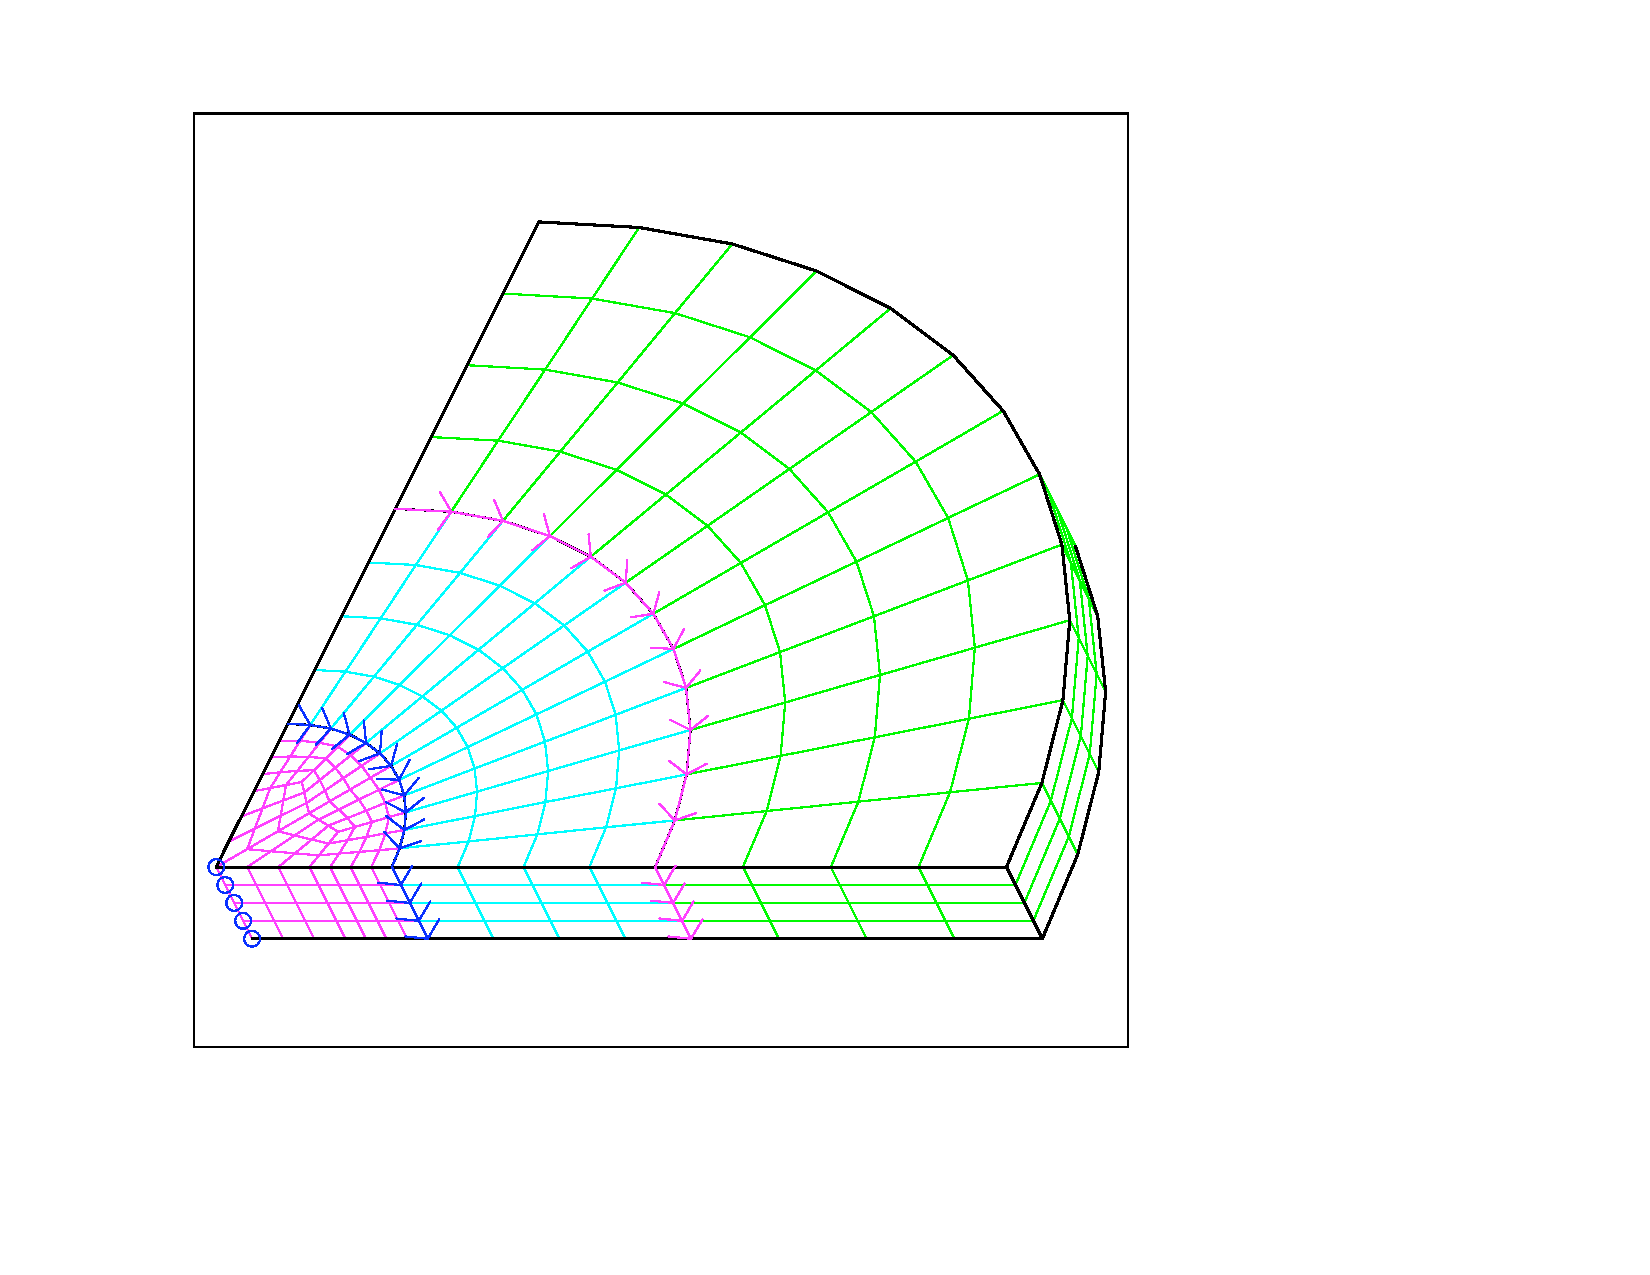
\includegraphics[width=3.0in]{figures/block_ss}
  \end{minipage}
  \caption [A \texttt{RADIAL TRISECTION} mesh with sidesets.] {Three dimensional \texttt{RADIAL TRISECTION} mesh with azimuthal
    angle of 90 degrees and two trisection blocks having sidesets
    specified on the radially outward directed faces of blocks 1 and 2. A nodeset is specified on the \textsc{ILO} face of this mesh and marks the edge corresponding to the z axis (blue circles).}
  \label{fig:block_ss}
\end{figure}

\clearpage
\subsection{User Defined Geometry Transformation}
\label{sec:inline-geometry-transform}
\index{User Defined Geometry Transformation}


{\ttfamily \small \begin{verbatim}
USER DEFINED GEOMETRY TRANSFORMATION
  "
    user supplied `C' language instructions;
  "
END
\end{verbatim}
}

The \texttt{USER DEFINED GEOMETRY TRANSFORMATION -- END} keyword pair provides
a powerful way to modify the coordinats of any node of a mesh. The keyword-end
pair must surround a double quote surrounded block of `C' code. This code will be called with coordinates of every node in the mesh. It may modify the the coordinats by setting the output variables \texttt{outxcoord}, \texttt{outycoord}, and \texttt{outzcoord}. The unmodified values of the node's coordinates are available in the input variables \texttt{inxcoord}, \texttt{inycoord}, and \texttt{inzcoord}.  The coordinates will remain unchanged if the output variables are not modified.  A presentation of the capabilities and
limitations of runtime compiled 'C' functions is included in
Appendix~\ref{sec:runtime-compiler-functionality}.

Examples of meshes produced using this capability feature of \textsc{pamgen} are shown below in Figure~\ref{fig:3d_transform_example} and Figure~\ref{fig:2d_transform_example}. In the first example the nodes with positive Z coordinate values are rotated about the Z axis an angle propportional to their distance from the Z=0 plane. In the second example nodes a distance of 0.5 from the origin are rotated about the origin in proportion to their distance from the origin.

\begin{figure}[t]
  \centering
    \begin{minipage}{0.3\linewidth}
{\ttfamily \begin{verbatim}






mesh
  rectilinear
    nx = 4
    ny = 4
    nz = 4
    bx =  3
    by =  3
    bz =  3
    gmin = -1.0 -1.0 -1.0
    gmax =  1.0  1.0  1.0
  end
  user defined geometry transformation
     "
     double r = sqrt(inxcoord*inxcoord+inycoord*inycoord);
     double theta = atan2(inycoord,inxcoord);
     if(inzcoord > 0.0)
      {
        theta = theta + (3.14159 / 4.0)*(inzcoord/1.0);
        r = r*(1.0-inzcoord/1.1);
        outxcoord = r*cos(theta);
        outycoord = r*sin(theta);
      }
     "
  end
end
\end{verbatim}}
    \end{minipage}%
    \hfill
    \begin{minipage}[t]{0.65\linewidth}
%      \centering
        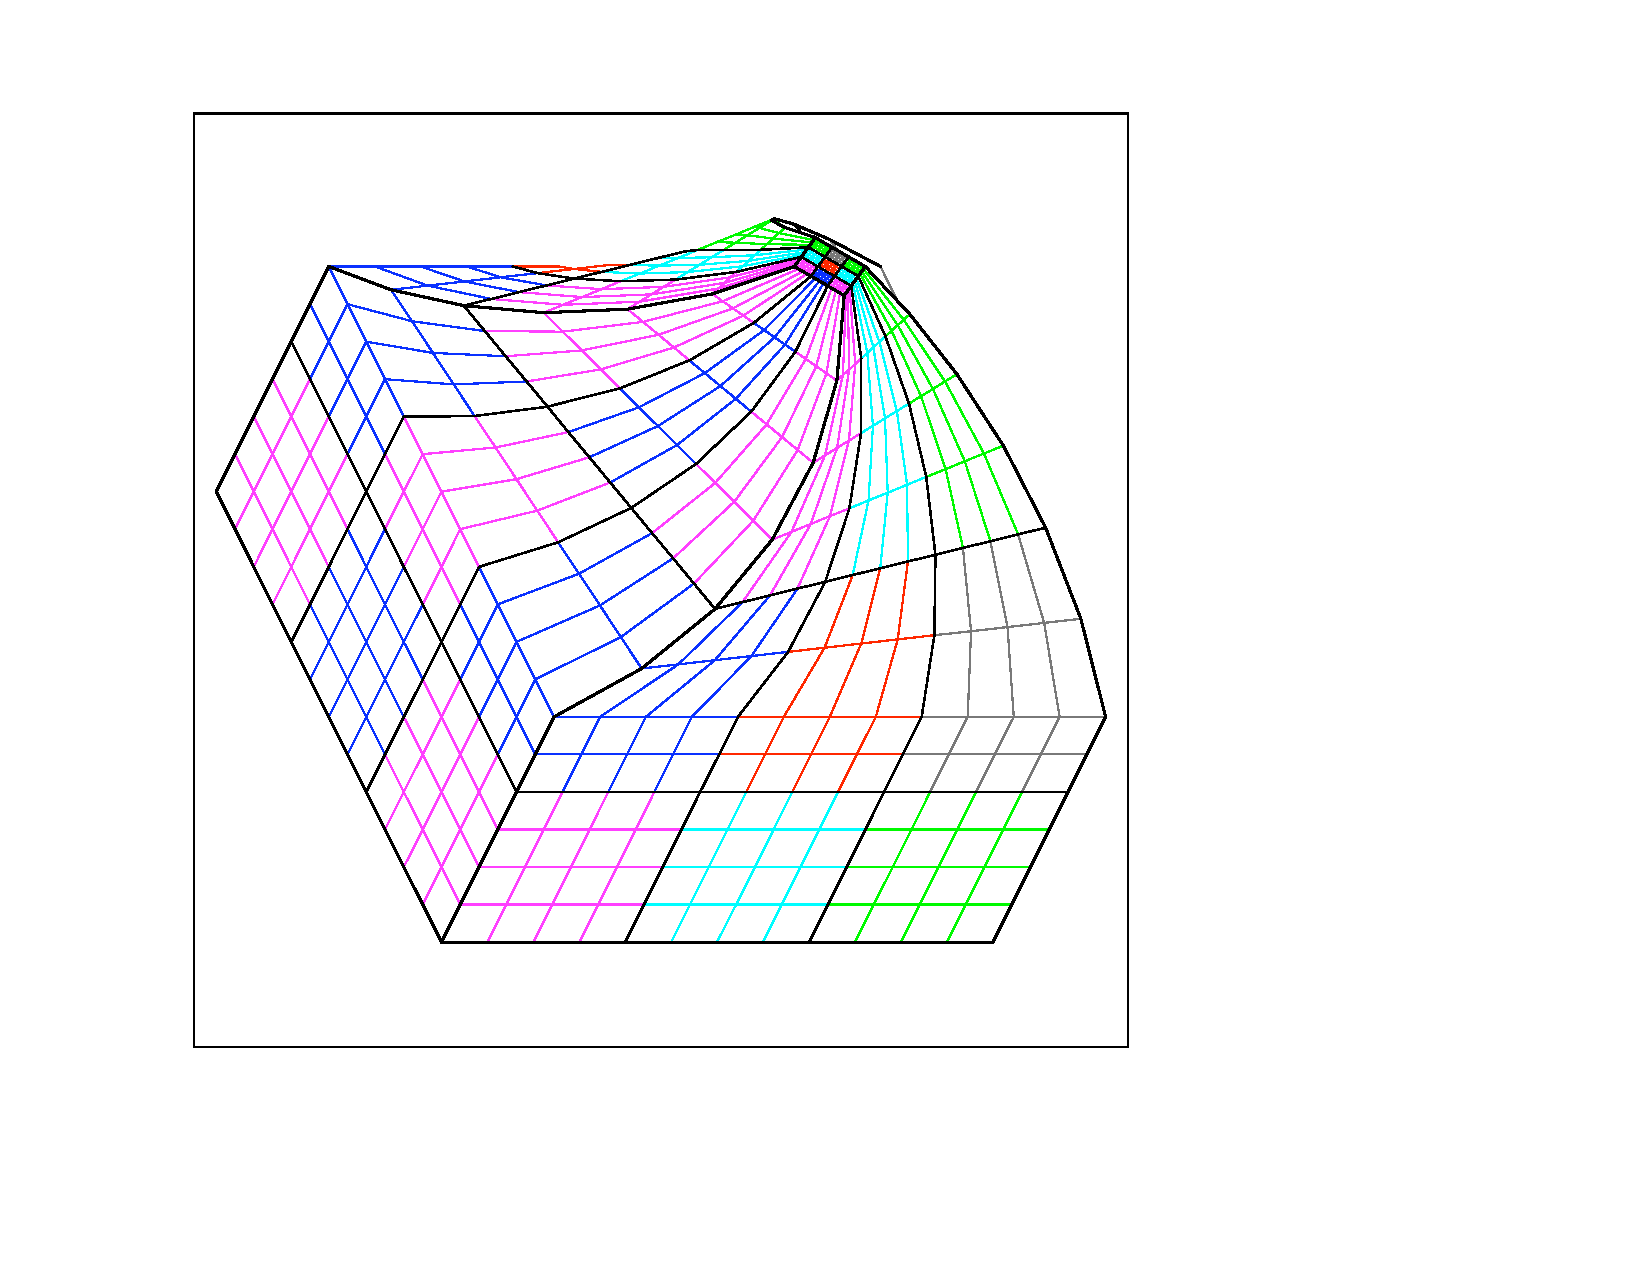
\includegraphics[width=4.8in]{figures/3d_warped_geometry_white_bg}
    \end{minipage}
 \caption [3D Geometry Transformation Example]{3D mesh illustrating the ability to modify nodal coordinates using \texttt{USER
      DEFINED GEOMETRY TRANSFORMATION}.}
    \label{fig:3d_transform_example}
\end{figure}


\begin{figure}[t]
  \centering
    \begin{minipage}{0.3\linewidth}
{\ttfamily \begin{verbatim}










mesh
  rectilinear
    nx = 10
    ny = 10
    bx =  3
    by =  3
    gmin = -1.0 -1.0
    gmax =  1.0  1.0
  end
  user defined geometry transformation
    "
    double r = sqrt(inxcoord*inxcoord+inycoord*inycoord);
    double theta = atan2(inycoord,inxcoord);
    if(r > 0.5)
     {
       theta = theta + (3.14159 / 4.0)*((r-0.5)/0.5);
       outxcoord = r*cos(theta);
       outycoord = r*sin(theta);
     }
    "
  end
end
\end{verbatim}}
    \end{minipage}%
    \hfill
    \begin{minipage}[t]{0.65\linewidth}
%      \centering
        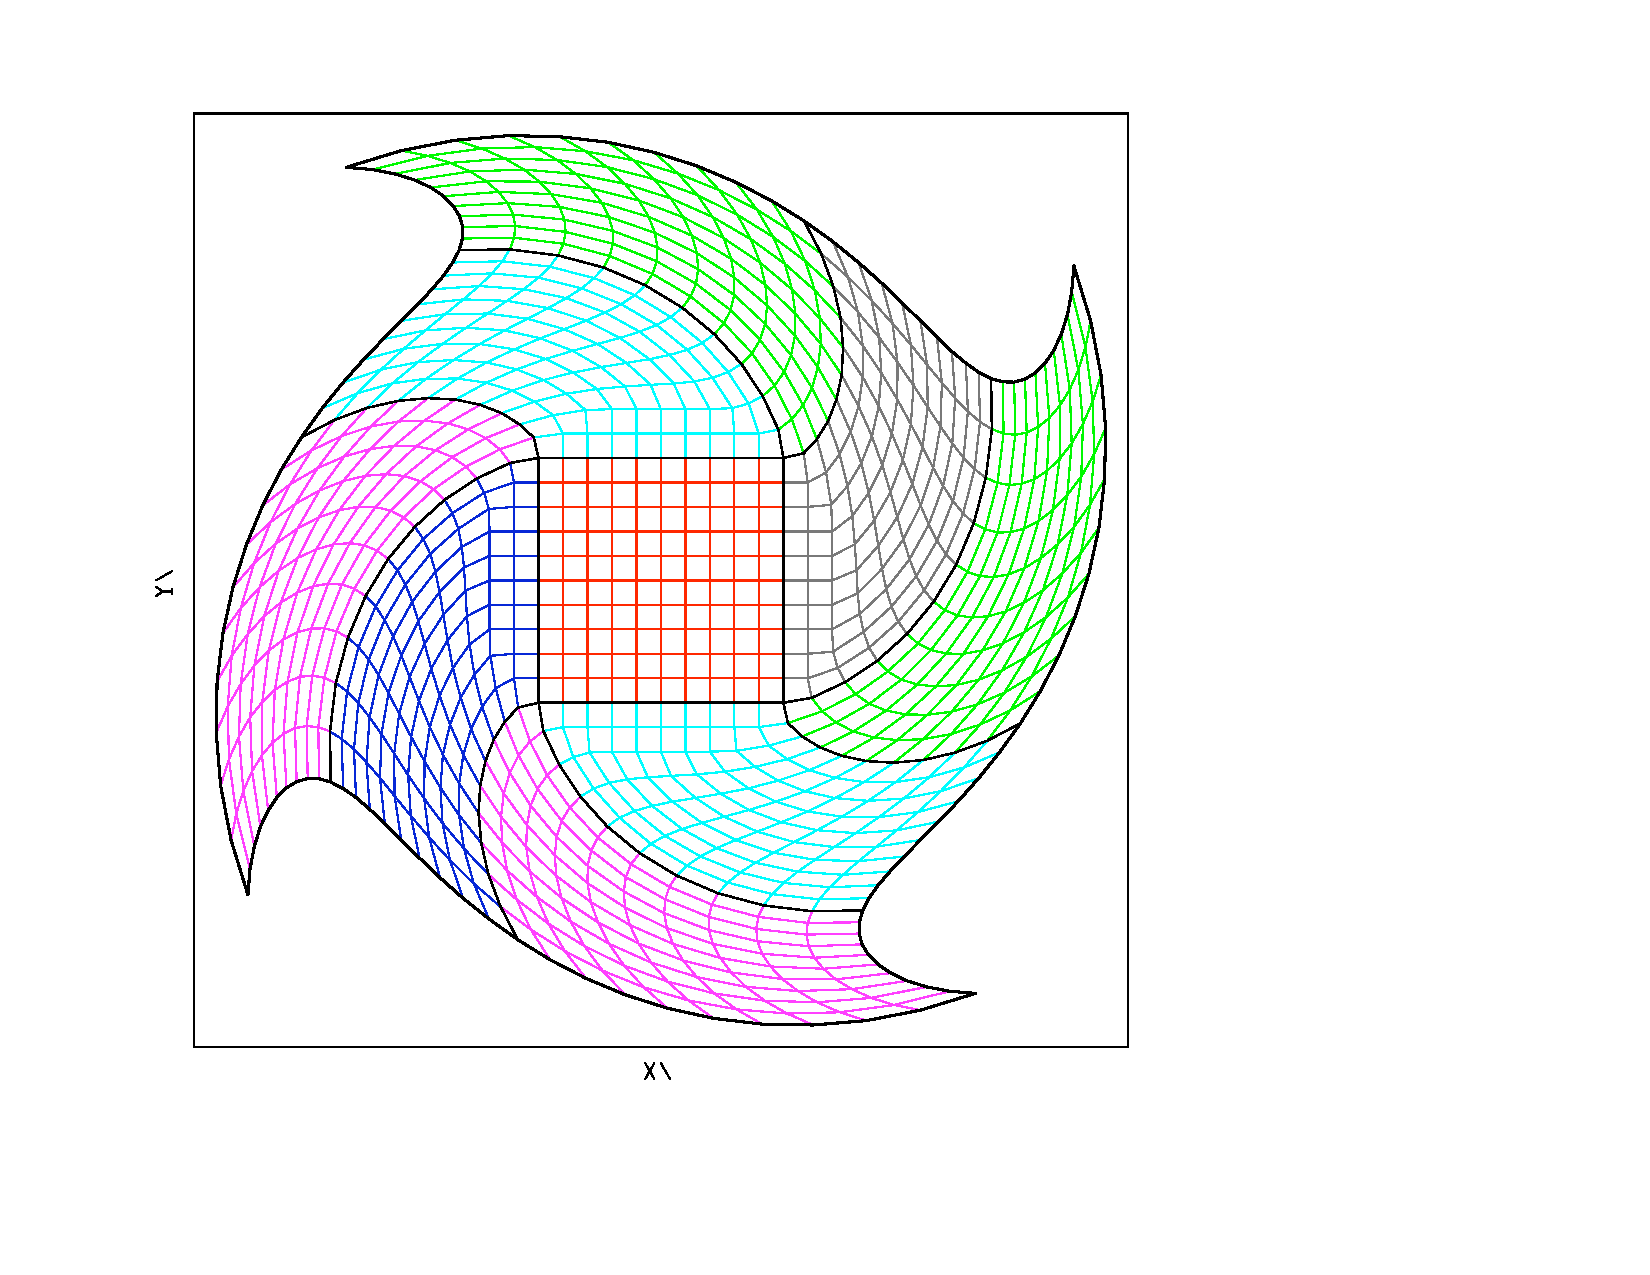
\includegraphics[width=3.8in]{figures/mesh_warp_2d_white_bg}
    \end{minipage}
    \caption [2D Geometry Transformation Example]{2D mesh illustrating the ability to modify nodal coordinates using \texttt{USER
      DEFINED GEOMETRY TRANSFORMATION}.}
    \label{fig:2d_transform_example}
\end{figure}


\clearpage
\subsection{User Defined Element Density}
\label{sec:inline-element-density}
\index{User Defined Element Density}


{\ttfamily \small \begin{verbatim}
USER DEFINED ELEMENT DENSITY, {I|J|K}
  "
    user supplied `C' language instructions;
  "
END
\end{verbatim}
}

The \texttt{USER DEFINED ELEMENT DENSITY -- END} keyword pair provides
a flexible way to bias \texttt{RECTILINEAR},
\texttt{SPHERICAL}, and \texttt{CYLINDRICAL} meshes. The keyword-end
pair must surround a double quote surrounded block of `C' code that
evaluates on the input variable \texttt{coord} and sets the return
value \texttt{field}. The return value \texttt{field} must be set to a
positive value across the range of the mesh in the selected
topological direction. A presentation of the capabilities and
limitations of runtime compiled 'C' functions is included in
Appendix~\ref{sec:runtime-compiler-functionality}.

The mesh biasing adjusts the nodal coordinates such that the density
of the elements in a region of the mesh in the selected coordinate
direction is proportional to the value of \texttt{field} relative to
the integral of \texttt{field} across the mesh domain. This is
implemented by numerically solving the equation given below. In this
equation \begin {math} x _ i \end {math} is the coordinate of node
\begin {math} i \end {math}, \begin {math} n \end {math} is the total
number of nodes in the coordinate direction, and \begin {math} f(u)
\end {math} is the user supplied function.

\begin{equation}
   \frac {\int _ {0} ^ {x _ i} f(u)du } {\int _ {0} ^ {x _ n} f(u)du }
   = \frac {i} {n}
\end{equation}

When these functions are applied to a two dimensional
\texttt{RECTILINEAR} mesh spanning from $(0.0, 0.0)$ to $(1.0, 1.0)$ and
having two blocks and 10 elements in both the 'I', and 'J' directions,
the resulting mesh is graded as shown in
Figure~\ref{fig:bias_example}.  The grading is a continuous
exponential function in the 'I' direction and is a discontinuous
function in the 'J' direction. In the 'J' direction the domain
stretching from 0.0 to 0.5 has twice the element density as the range
from 0.5 to 1.0.
%\clearpage

Diagnostic information for the user provided functions is included in
the \texttt{runid.out} file.  This information includes the total
integrated value of the function, the minimum and maximum value of the
function, and a plot of the function's values across the range of
evaluation.

\begin{figure}[htbp]
  \centering
    \begin{minipage}{0.5\linewidth}
{\ttfamily \begin{verbatim}
user defined element density, i
  "
    field = 1.*exp(-5.*(coord));
  "
end
user defined element density, j
  "
    field = 1;
    if(coord < 0.5)  { field = 2;}
    if(coord >= 0.5) { field = 1;}
  "
end
\end{verbatim}}
    \end{minipage}%
    \hfill
    \begin{minipage}{0.45\linewidth}
      \centering
        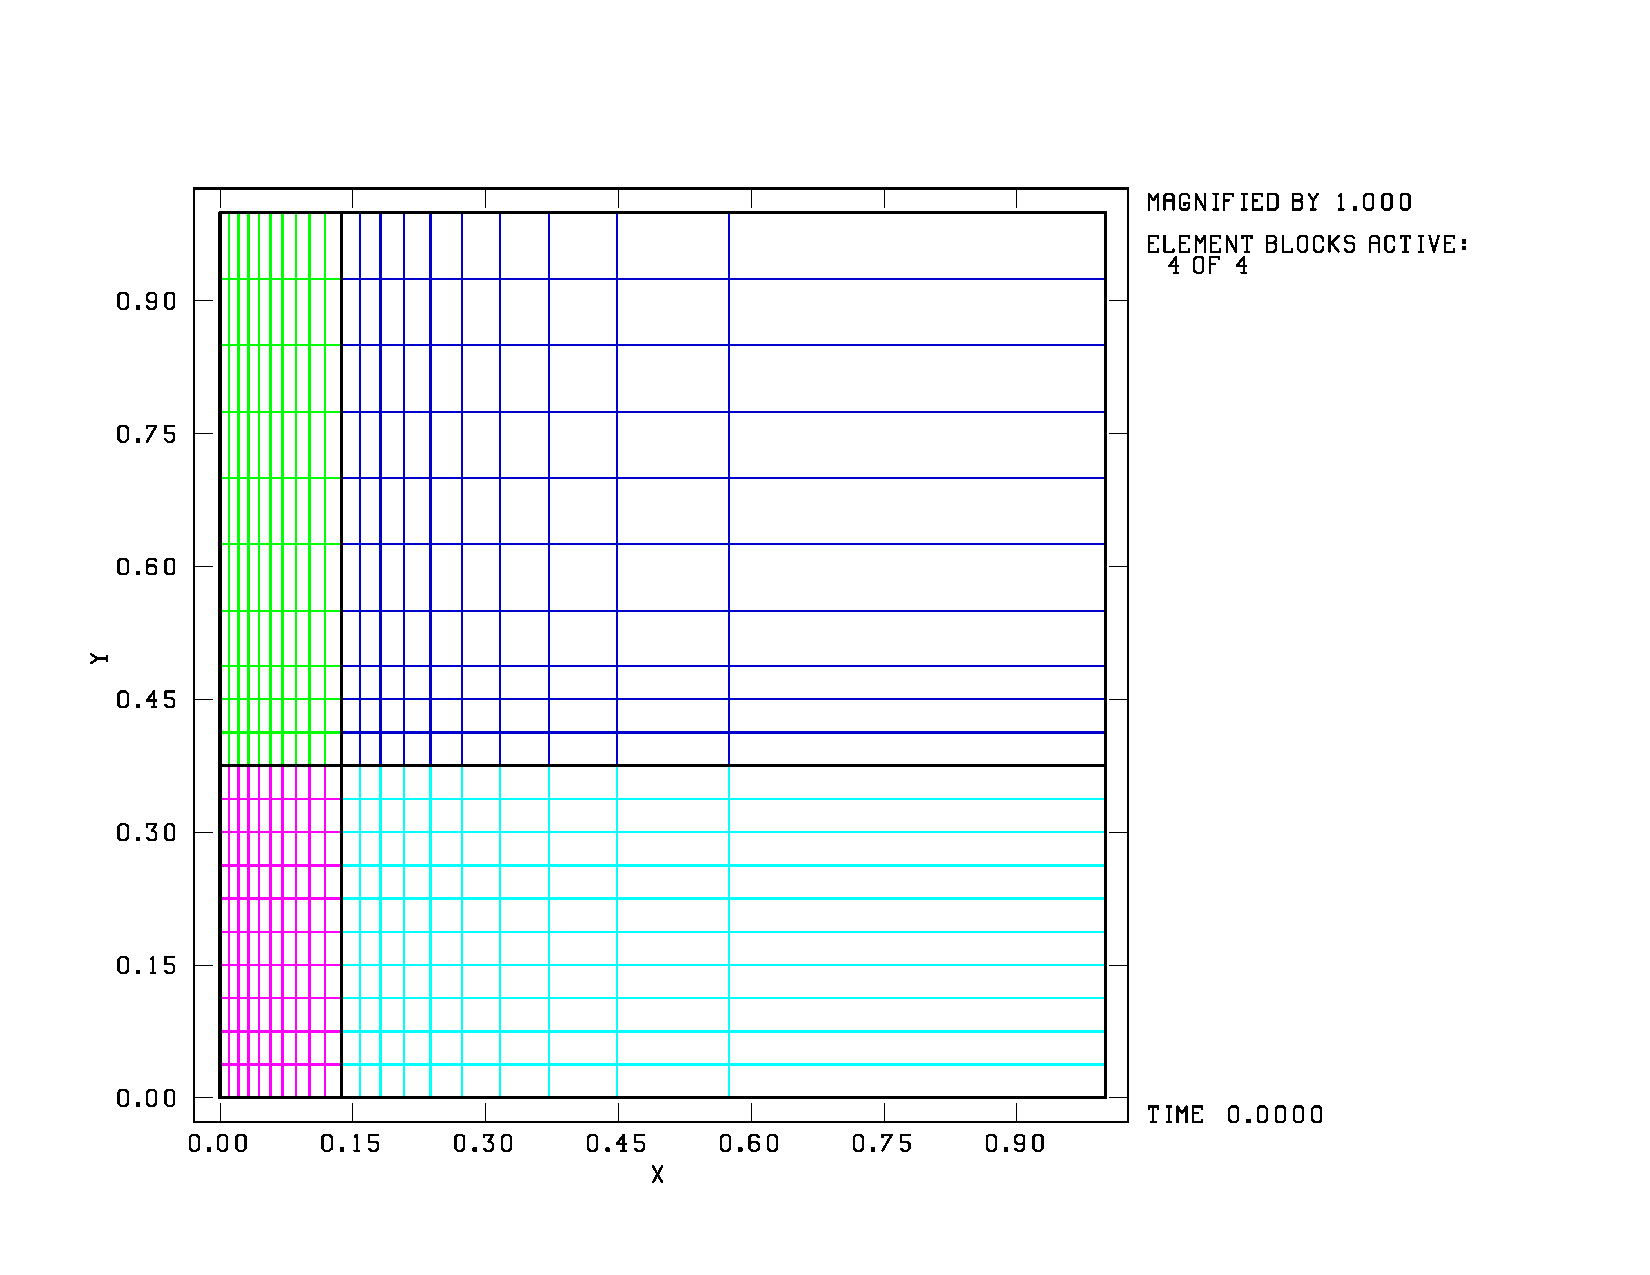
\includegraphics[width=2.8in]{figures/bias_example}
    \end{minipage}
    \caption{2D mesh created with a \texttt{USER
      DEFINED ELEMENT DENSITY}.}
    \label{fig:bias_example}
\end{figure}

\renewcommand{\textfraction}{0.2}
\renewcommand{\topfraction}{0.7}
\renewcommand{\bottomfraction}{0.3}
\renewcommand{\floatpagefraction}{0.5}

\clearpage
\subsection{Decomposition Strategy}
\label{sec:inline-decomposition-strategy}
\index{Decomposition Strategy}

{\ttfamily \begin{verbatim}
DECOMPOSITION STRATEGY
   {BISECTION}
   {PROCESSOR LAYOUT}
     {NUMPROCS, I, int (1)}
     {NUMPROCS, J, int (1)}
     {NUMPROCS, K, int (1)}
   {END}
   {SEQUENTIAL}
   {RANDOM}
END
\end{verbatim}
}

An optional \texttt{DECOMPOSITION STRATEGY -- END} block pair surrounds the description
of the decomposition method used for parallel simulations. The default strategy is \texttt{BISECTION}. The keywords associated
with the \texttt{DECOMPOSITION STRATEGY} keyword are given in
Table~\ref{tab:inlinemesh-decomp_strat}.

\mthreecolumntable{
  Keywords for \texttt{DECOMPOSITION STRATEGY -- END}.
  \label{tab:inlinemesh-decomp_strat}
}{
\hline
  Sub-Keyword & Input & Description \\

\hline \hline
  \smallskip \texttt{BISECTION} & &
       Recursively bisect domain making slices calculated to assign nearly equal numbers of elements to each processor. This option is the default. \\ \hline \smallskip
  \begin{minipage} [c]{1.0\linewidth} \setlength{\parindent}{0.1in} \noindent \texttt{PROCESSOR LAYOUT} \\ \indent \texttt{NUMPROCS \{I|J|K\}}, int (1)  \\ \texttt{END} \end{minipage}  & \texttt{int} (1)&
       Invokes a decomposition strategy that slices up the mesh in accordance with the request of the user.  The integer value value is number of segments into which the mesh should be divided in
       the given direction. The product of the number of segments requested in each direction must equal the number of processors.  \\ \hline
  \smallskip \texttt{SEQUENTIAL} & &
       Invokes a decomposition strategy that distributes the elements between processors in sequential order. If there are k elements and n processors an average of k/n elements will go to each processor. \emph{This decomposition strategy is not for large simulations and is intended mainly for testing and verification purposes.}  \\ \hline
  \smallskip \texttt{RANDOM} & &
       Invokes a decomposition strategy that randomly distributes the elements between processors. It results in tremendous communications overhead. \emph{This decomposition strategy is not for production simulations and is intended mainly for testing and verification purposes.}\\ \hline
}

The \texttt{BISECTION} decomposition strategy is the default for parallel calculations. This is
because it is robust in providing decompositions and the resulting
regions have satisfactory surface area to volume ratios. This strategy
attempts to automatically determine the number of slices to make through
the entire mesh domain to provide an equal number of elements to each processor. This strategy will be most successful when the number of processors, and the number of elements in each direction are a power of 2 or a product of several prime numbers.

The \texttt{PROCESSOR LAYOUT} decomposition strategy offers the user
improved control of the distribution of elements to each
processor in a parallel simulation. The strategy divides the mesh into the number of segments specified by the keyword-value pair for each coordinate direction. The number of
processors must equal the product of the values given for each of the
\texttt{NUMPROCS} directions. The default value for a coordinate direction is one.

When using a \texttt{RADIAL TRISECTION} mesh the number of processors in the \texttt{I} (radial) direction is fixed at 1, and the total number of processors must be equal to the
product of the values given for the \texttt{J} and \texttt{K}
\texttt{NUMPROCS} directions. For this mesh type the decomposition
assigns elements from the inner transition blocks to the processor
that owns the adjacent elements in the outer cylinderical blocks.
An example of the \texttt{PROCESSOR LAYOUT} decomposition option
applied to a \texttt{RADIAL TRISECTION} mesh is shown in Figure \ref{fig:tri_dec}.

Examples of \texttt{BISECTION} and
\texttt{PROCESSOR LAYOUT} decomposition options applied to a mesh definition with the
\texttt{RADIAL} option are shown below in
Figures~\ref{fig:dec_bis} and
 \ref{fig:dec_pl}. The total
number of elements in this problem was 204, 17 in the radial or
\texttt{I} direction and 12 in the azimuthal or \texttt{J} direction.

For the \texttt{BISECTION} decomposition the recursive cuts made on
the 17x12x1 array of elements results in three processors with 3x12x1 elements,
four processors with 2x12x1
elements and a single processor 6x8x1 elements.

For the \texttt{PROCESSOR LAYOUT} decomposition the
17 elements in the \texttt{I} or radial direction are divided by 4 to
set the size of segments produced in that direction at 4. The first segment's size is increased by one to handle the remainder of dividing 14 by 4. This decomposition would equally
distribute elements to each processor if the \texttt{I} direction had a number of
elements evenly divisible by 4.

\begin{figure}[htbp]
\centering
  \begin{minipage}[c]{0.4\linewidth}
    \centering
{\ttfamily \begin{verbatim}
mesh
  radial
    numz 1
      zblock 1 10.0 interval 1
    numr 4 initial radius 1.
      rblock 1 2. interval 3
      rblock 2 4. interval 3
      rblock 3 6. interval 5
      rblock 4 8. interval 6
    numa 1
      ablock 1 60. interval 12
  end
  decomposition strategy
    bisection
  end
end
\end{verbatim}}
  \end{minipage}%
  \hfil
  \begin{minipage}[c]{0.6\linewidth}
    \centering
      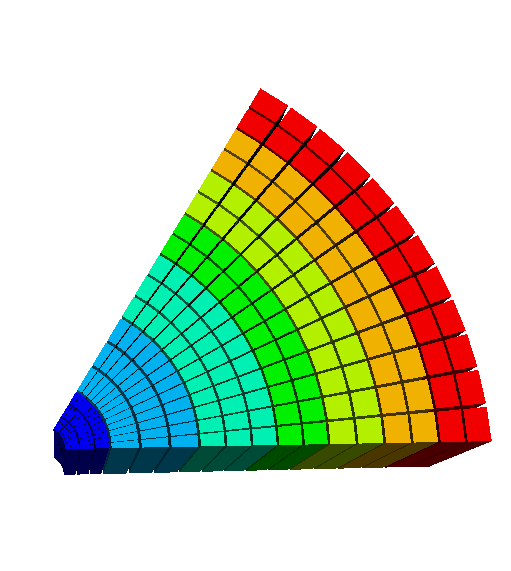
\includegraphics[width=2.0in]{figures/bisect_7_white}
  \end{minipage}
  \caption [\texttt{BISECTION} decomposition run on 7 processors.] {Three dimensional \texttt{RADIAL} mesh with azimuthal
    angle of 60 degrees run on 7 processors using \texttt{BISECTION} decomposition.}
  \label{fig:dec_bis}
\end{figure}


\begin{figure}[htbp]
\centering
  \begin{minipage}[c]{0.4\linewidth}
    \centering
{\ttfamily \begin{verbatim}
mesh
  radial
    numz 1
      zblock 1 10.0 interval 1
    numr 4 initial radius 1.
      rblock 1 2. interval 3
      rblock 2 4. interval 3
      rblock 3 6. interval 5
      rblock 4 8. interval 6
    numa 1
      ablock 1 60. interval 12
  end
  decomposition strategy
    numprocs i, 4
    numprocs j, 2
  end
end
\end{verbatim}}
  \end{minipage}%
  \hfil
  \begin{minipage}[c]{0.6\linewidth}
    \centering
      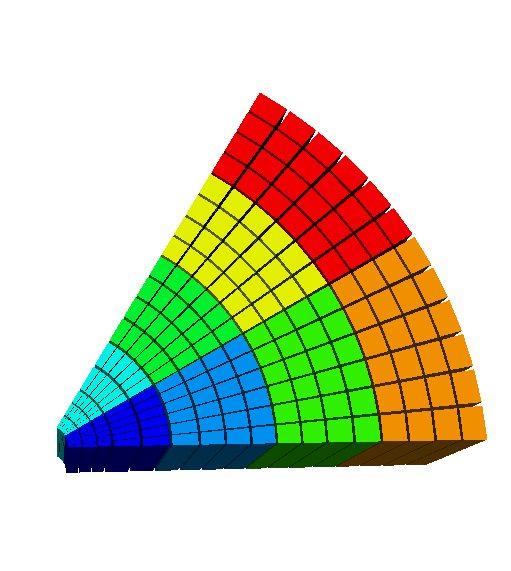
\includegraphics[width=2.0in]{figures/numprocs_8}
  \end{minipage}
  \caption [\texttt{PROCESSOR LAYOUT} decomposition run on 8 processors.] {Three dimensional \texttt{RADIAL} mesh with azimuthal
    angle of 60 degrees run on 8 processors using \texttt{PROCESSOR LAYOUT} decomposition.}
  \label{fig:dec_pl}
\end{figure}
\begin{figure}[htbp]
\centering
  \begin{minipage}[c]{0.4\linewidth}
    \centering
{\ttfamily \begin{verbatim}
mesh
  radial trisection
    trisection blocks, 4
    numz 1
      zblock 1 4.0 interval 1
    numr 3
       rblock 1 2. interval 4
       rblock 2 3. interval 4
       rblock 3 5. interval 4
    numa 1
      ablock 1 360. interval 32
  end
  decomposition strategy
    numprocs j, 8
  end
end
\end{verbatim}}
  \end{minipage}%
  \hfil
  \begin{minipage}[c]{0.6\linewidth}
    \centering
      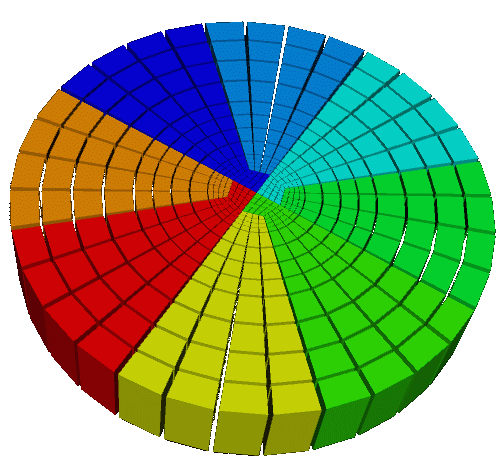
\includegraphics[width=2.0in]{figures/trisection_decomp}
  \end{minipage}
  \caption [\texttt{PROCESSOR LAYOUT} decomposition on 8 processors.] {Three dimensional \texttt{RADIAL TRISECTION} mesh run on 8 processors using \texttt{PROCESSOR LAYOUT} decomposition.}
  \label{fig:tri_dec}
\end{figure}


\clearpage
\section{Library Interface}\label{sec:execution_steps}
\subsection{Creating a Mesh}
Mesh creation proceeds through a single function call. Additional functions are available to access messages generated during the mesh creation.
\subsubsection{Create\_Pamgen\_Mesh}
{\ttfamily  \begin{verbatim}
int Create_Pamgen_Mesh( char * file_char_array,
                        int dimension,
                        int rank,
                        int num_procs);
\end{verbatim}}
This function creates a representation of the mesh for the processor of the specified rank out of the total num\_procs. It returns an enumerated value. A return value of \textbf{ERROR\_FREE\_CREATION
} signifies success. A return value of \textbf{ERROR\_CREATING\_IMD} significes an error in the specification of the mesh geometry, topology, or boundary conditions. A return value of \textbf{ERROR\_CREATING\_MS} significes an error in allocating and populating the arrays that store the mesh geometry and topology. A return value of \textbf{ERROR\_PARSING\_DEFINITION} significes an error occurred while parsing the string passed in file\_char\_array. The details of the syntax error are recoverable by subsequent calls.

%\begin{itemize}
{
\setlength{\parindent}{0pt}

 \textbf{char *file\_char\_array}
This input variable points to a null terminated string that holds a terse description of the desired mesh.  This form of this description is given in a later section.

 \textbf{int dimension}
This input variable indicates the dimension of the desired mesh. Acceptable values are 2 (quadrilaterals created in x,y plane) and 3 (hexahedral elements created in 3 space).

 \textbf{int rank}
This input variable may range from 0 to one less than num\_procs. It specifies for which processor the mesh is being generated.

 \textbf{int num\_procs}
This input variable must be greater than 0.  It specifes the total number of processors across which the mesh is decomposed.
}
%\end{itemize}
\subsubsection{getPamgenEchoStreamSize}
{\ttfamily  \begin{verbatim}
int getPamgenEchoStreamSize(void);
\end{verbatim}}

This function returns the size of the string (not counting termination character) that contains an echo of the \textbf{char * file\_char\_array} string previously passed to Create\_Pamgen\_Mesh. If a parsing error occurred, this string will be annotated with a summary of the error. Use of this function and subsequent access and display of this string is highly recommended if the value pointed to by \textbf{int * parse\_error\_count} is non-zero on return.

\subsubsection{getPamgenEchoStream}
{\ttfamily  \begin{verbatim}
char * getPamgenEchoStream(char * echo_stream_pointer);
\end{verbatim}}
This function takes a character pointer and returns that same pointer after it has been filled.

{\setlength{\parindent}{0pt}
 \textbf{char *echo\_stream\_pointer} This input variable must point to allocated memory big enough to hold the the results of ``getEchoStreamSize(void)'' plus a termination character.
}

\subsubsection{getPamgenErrorStreamSize}
{\ttfamily  \begin{verbatim}
int getPamgenErrorStreamSize(void);
\end{verbatim}}
This function returns the size of an error string associated with a return value of \textbf{ERROR\_CREATING\_MS} from Create\_Pamgen\_Mesh.


\subsubsection{getPamgenErrorStream}
{\ttfamily  \begin{verbatim}
char * getPamgenErrorStream(char * error_stream_pointer);
\end{verbatim}}
This function takes a character pointer and returns that same pointer after it has been filled.

{\setlength{\parindent}{0pt}
 \textbf{char *error\_stream\_pointer} This input variable must point to allocated memory big enough to hold the the results of getErrorStreamSize plus a termination character.
}


\subsubsection{getPamgenWarningStreamSize}
{\ttfamily  \begin{verbatim}
int getPamgenWarningStreamSize(void);
\end{verbatim}}
This function returns the size of a string containing warnings generated within the Create\_Pamgen\_Mesh function.

\subsubsection{getPamgenWarningStream}
{\ttfamily  \begin{verbatim}
char * getPamgenWarningStream(char * warning_stream_pointer);
\end{verbatim}}
This function takes a character pointer and returns that same pointer after it has been filled.

{\setlength{\parindent}{0pt}
 \textbf{char *warning\_stream\_pointer} This input variable must point to allocated memory big enough to hold the the results of getWarningStreamSize plus a termination character.
}

\subsubsection{getPamgenInfoStreamSize}
{\ttfamily  \begin{verbatim}
int getPamgenInfoStreamSize(void);
\end{verbatim}}
This function returns the size of a string containing information messages generated within the Create\_Pamgen\_Mesh function. These messages include information such as the total number of elements in the mesh, the total number of nodes in the mesh, and the mesh distribution based on decomposition.

\subsubsection{getPamgenInfoStream}
{\ttfamily  \begin{verbatim}
char * getPamgenInfoStream(char * info_stream_pointer);
\end{verbatim}}
This function takes a character pointer and returns that same pointer after it has been filled.

{\setlength{\parindent}{0pt}
 \textbf{char *info\_stream\_pointer} This input variable must point to allocated memory big enough to hold the the results of getInfoStreamSize plus a termination character.
}
\clearpage
\subsection{Querying a Mesh}
All of the mesh query and access functions are based on the \texttt{EXODUS II} ~\cite{Schoof-Yarberry:1995} and \texttt{NEMESIS} ~\cite{Hennigan-StJohn-Shadid:1998} APIs. These APIs were written to standardize a platform independent interface for writing and reading binary mesh specification files. \texttt{NEMESIS} is a parallel extension of the serial \texttt{EXODUS II} API.  The \textsc{pamgen} function names are formed by prefixing the \texttt{EXODUS II} or \texttt{NEMESIS} function name with \textbf{im\_}. The remainder of the function signature and functionality remains unchanged. It may help to note that the original \texttt{EXODUS II} functions begin with \textbf{ex\_}, and the original \texttt{NEMESIS} functions begin with \textbf{ne\_}.

Querying a mesh database to build up a complete representation in accessible memory is a straightforward process.  Typically a query function is used to ascertain the number of items in an array, then memory is allocated and passed in through an access function which fills the memory with the requested information. The query and access functions will be presented in the same order they appear in the example function ``read\_mesh\_to\_memory()'' shown in Appendix~\ref{sec:read-mesh-to-memory}.


\subsubsection{im\_ex\_get\_init}
{\ttfamily  \begin{verbatim}
int im_ex_get_init( int exoid,
                    char *title,
                    int  *num_dim,
                    int  *num_nodes,
                    int  *num_elem,
                    int  *num_elem_blk,
                    int  *num_node_sets,
                    int  *num_side_sets);
\end{verbatim}}
This function is based on the \texttt{EXODUS II} API and is concerned only with serial information. The number of nodes, elements, element blocks is limited to those entities local to the rank processor for which the mesh was created. It returns a non-zero value if an error occurs.

{\setlength{\parindent}{0pt}
 \textbf{int exoid} An unused input variable.\par
 \textbf{char *title} A title string containing ``PAMGEN Inline Mesh''.\par
 \textbf{char *num\_dim} On return points to the number of coordinates per node (2 or 3).\par
 \textbf{char *num\_nodes} On return points to the number of nodes.\par
 \textbf{char *num\_elem} On return points to the number of elements.\par
 \textbf{char *num\_elem\_blk} On return points to the number of element blocks.\par
 \textbf{char *num\_node\_sets} On return points to the number of node sets.\par
 \textbf{char *num\_side\_sets} On return points to the number of side sets.\par
}

\subsubsection{im\_ex\_inquire}
{\ttfamily  \begin{verbatim}
int im_ex_inquire( int exoid,
                   int query_value,
                   int *int_value,
                   float *float_value,
                   char * char_array_value);
\end{verbatim}}
This function is based on the \texttt{EXODUS II} API and is concerned only with serial information. This is a general purpose query function that takes an enumerated query value and changes the value pointed to by int\_value, float\_value, or char\_array\_value depending on the data requested by the query\_value. It returns a non-zero value in case of error. Im\_ex\_inquire supports the following query values:
\begin{itemize}\addtolength{\itemsep}{-0.5\baselineskip}\renewcommand{\labelitemi}{}
	\item \textbf{IM\_EX\_INQ\_NS\_NODE\_LEN} The length of the concatenated nodeset list is returned in int\_value.
  	\item \textbf{IM\_EX\_INQ\_NS\_DF\_LEN} The length of the concatenated nodeset distribution list is returned in int\_value.
  	\item \textbf{IM\_EX\_INQ\_SS\_ELEM\_LEN} The length of the concatenated sidesets element list is returned in int\_value.
  	\item \textbf{IM\_EX\_INQ\_SS\_NODE\_LEN} The aggregate length of the sideset nodes is returned in int\_value.
  	\item \textbf{IM\_EX\_INQ\_SS\_DF\_LEN } The length of the concatenated side sets distribution factor is returned in int\_alue.
  	\item \textbf{IM\_EX\_INQ\_API\_VERS} The API version is returned in float\_value.
	\item \textbf{IM\_EX\_INQ\_EB\_PROP} The number of element block properties is returned in int\_value.
	\item \textbf{IM\_EX\_INQ\_NS\_PROP} The number of node sets properties is returned in int\_value.
	\item \textbf{IM\_EX\_INQ\_SS\_PROP} The number of side set properties is returned in int\_value.
	\item \textbf{IM\_EX\_INQ\_QA} The number of QA records is returned in int\_value.
	\item \textbf{IM\_EX\_INQ\_INFO} The number of INFO records is returned in int\_value.

\end{itemize}

\subsubsection{im\_ex\_get\_coord}
{\ttfamily  \begin{verbatim}
int im_ex_get_coord( int exoid,
                     double* x_coors,
                     double* y_coors,
                     double* z_coors);
\end{verbatim}}
This function is based on the \texttt{EXODUS II} API and is concerned only with serial information. This function takes pointers to memory allocated to a length equal to the number of nodes local to the processor and fills in the nodal coordinate values. A non-zero return value indicates an error.

{\setlength{\parindent}{0pt}
 \textbf{int exoid} Unused input variable.}

{\setlength{\parindent}{0pt}
 \textbf{double * x\_coors} Returned X coordinates of the nodes.}

{\setlength{\parindent}{0pt}
 \textbf{double * y\_coors} Returned Y coordinates of the nodes.}

{\setlength{\parindent}{0pt}
 \textbf{double * z\_coors} Returned Z coordinates of the nodes (if num\_dim = 3).}


\subsubsection{im\_ex\_get\_coord\_names}
{\ttfamily  \begin{verbatim}
int im_ex_get_coord_names( int exoid,
                           char ** coord_names);
\end{verbatim}}
This function is based on the \texttt{EXODUS II} API and is concerned only with serial information. It returns the names of the coordinates. A non-zero return indicates an error.

{\setlength{\parindent}{0pt}
 \textbf{int exoid} Unused input variable.}

{\setlength{\parindent}{0pt}
 \textbf{char ** coord\_names} Returned vector pointing to num\_dim coord names. \textbf{coord\_names} can be declared and allocated as shown below.}
{\ttfamily  \begin{verbatim}
char* coord_names[3];
for(int i = 0; i < num_dim; i++)
   coord_names[i] = (char*)calloc((MAX_STR_LENGTH+1),sizeof(char));
\end{verbatim}}

\subsubsection{im\_ex\_get\_map}
{\ttfamily  \begin{verbatim}
int im_ex_get_map( int exoid,
                   int * element_map);
\end{verbatim}}
This function is based on the \texttt{EXODUS II} API and is concerned only with serial information. It loads the global element numbers into the provided storage. A non-zero return value indicates an error.

{\setlength{\parindent}{0pt}
 \textbf{int exoid} Unused input variable.}

{\setlength{\parindent}{0pt}
 \textbf{int * element\_map} On return this array holds the global element ids of the elements local to this processor. For a serial problem this runs sequentially from 1 to num\_elem. Memory sized to num\_elem must be allocated prior to making this call.}

\subsubsection{im\_ex\_get\_elem\_num\_map}
{\ttfamily  \begin{verbatim}
int im_ex_get_elem_num_map( int exoid,
                            int * element_num_map);
\end{verbatim}}
For \textsc{pamgen} this function is identical to ``im\_ex\_get\_map''.

{\setlength{\parindent}{0pt}
 \textbf{int exoid} Unused input variable.}

{\setlength{\parindent}{0pt}
 \textbf{int * element\_num\_map}  On return this array holds the global element ids of the elements local to this processor. For a serial problem these values run sequentially from 1 to num\_elem. Memory sized to num\_elem must be allocated prior to making this call.}

\subsubsection{im\_ex\_get\_node\_num\_map}
{\ttfamily  \begin{verbatim}
int im_ex_get_node_num_map( int exoid,
                            int * node_num_map);
\end{verbatim}}
This function is based on the \texttt{EXODUS II} API and is concerned only with serial information. It loads the global node numbers into the provided storage. A non-zero return indicates an error.

{\setlength{\parindent}{0pt}
 \textbf{int exoid} Unused input variable.}

{\setlength{\parindent}{0pt}
 \textbf{int * node\_num\_map}  On return this array holds the global node ids of the nodes local to this processor. For a serial problem this runs from 1 to num\_nodes. Memory sized to num\_nodes must be allocated prior to making this call.}
%element block ids
\subsubsection{im\_ex\_get\_elem\_blk\_ids}
{\ttfamily  \begin{verbatim}
int im_ex_get_elem_blk_ids( int exoid,
                            int * elem_blk_ids);
\end{verbatim}}
This function is based on the \texttt{EXODUS II} API and is concerned only with serial information. It loads the element block ids into the provided storage. A non-zero return value indicates an error.

{\setlength{\parindent}{0pt}
 \textbf{int exoid} Unused input variable.}

{\setlength{\parindent}{0pt}
 \textbf{int * elem\_blk\_ids}  On return this array holds the ids of the element blocks on this processor. For \textsc{pamgen} meshes the element block ids across the entire problem will run sequentially from 1 to num\_elem\_blk. On any particular processor of a parallel mesh any set of the global element blocks may be present. Storage sized to num\_elem\_blk must be allocated prior to making this call.}

\subsubsection{im\_ex\_get\_elem\_block}
{\ttfamily  \begin{verbatim}
int im_ex_get_elem_block( int exoid,
                          int elem_blk_id,
                          char * elem_type,
                          int * num_elem_this_blk,
                          int * num_nodes_per_elem,
                          int * num_attr);
\end{verbatim}}
This function is based on the \texttt{EXODUS II} API and is concerned only with serial information. It provides information about the requested element block.  Review of the conventions documented in the \texttt{EXODUS II} manual is the most effective way to understand the mesh storage and retrieval. Under the \texttt{EXODUS II} convention, a finite element mesh is composed of one or more blocks of elements. Each block contains elements of the same type. Within a block, all elements have the same number of nodes and the same connectivity convention. The number of nodes is stored explicitly, and the connectivity convention is called out by a string. This string corresponds to a table of conventional element connectivities in the \texttt{EXODUS II} manual. A non-zero return value indicates an error.

{\setlength{\parindent}{0pt}
 \textbf{int exoid} Unused input variable.}

{\setlength{\parindent}{0pt}
 \textbf{int elem\_blk\_id}  Input variable specifying the id of the block for which information is requested. This id must be one of the values in the elem\_blk\_ids array.}

{\setlength{\parindent}{0pt}
 \textbf{char * elem\_type}  On return this variable holds one of the standard \texttt{EXODUS II} element types as a string. The element\_type pointer must be allocated as length MAX\_STR\_LENGTH+1. For \textsc{pamgen} the stored value will be QUAD in 2D or HEX in 3D.}

{\setlength{\parindent}{0pt}
 \textbf{int * num\_elem\_this\_blk}  On return this variable holds the number of elements in this block. }

{\setlength{\parindent}{0pt}
 \textbf{int * num\_nodes\_per\_elem}  On return this variable holds the number of nodes per element for the elements in this block. }

{\setlength{\parindent}{0pt}
 \textbf{int * num\_attr}  On return this variable holds the number of attributes for this block for \textsc{pamgen} this is always 0. }

\subsubsection{im\_ex\_get\_elem\_conn}
{\ttfamily  \begin{verbatim}
int im_ex_get_elem_conn( int exoid,
                         int elem_blk_id,
                         int * connect);
\end{verbatim}}
This function is based on the \texttt{EXODUS II} API and is concerned only with serial information. It fills the storage pointed to by connect with the connectivity of the elements in the block referred to by elem\_blk\_id. A non-zero return value indicates an error.

{\setlength{\parindent}{0pt}
 \textbf{int exoid} Unused input variable.}

{\setlength{\parindent}{0pt}
 \textbf{int elem\_blk\_id}  Input variable specifying the id of the block for which information is requested. This id must be one of the values in the elem\_blk\_ids array.}

{\setlength{\parindent}{0pt}
 \textbf{int * connect}  On return the storage pointed to by \textbf{connect} holds the connectivity for the requested block. \textbf{Connect} must point to storage sized to num\_elem\_this\_block*num\_nodes\_per\_elem. \textbf{Connect} holds (in the order specified by the \texttt{EXODUS II} convention) the nodes of each element in the specified block. The first element's connectivity begins at an offset of 0 and the nth element's connectivity begins at an offset of n*num\_nodes\_per\_element. The \texttt{EXODUS II} standard specifies that the indices of the connectivity are numbered  from 1 so that in order to retrieve the coordinates of an element's nodes the indices given in \textbf{connect} must be decrimented by 1.}

\subsubsection{im\_ex\_get\_node\_set\_ids}
{\ttfamily  \begin{verbatim}
int im_ex_get_node_set_ids( int exoid,
                            int * node_set_ids);
\end{verbatim}}
This function is based on the \texttt{EXODUS II} API and is concerned only with serial information. It loads the node set ids into the provided storage. Node set ids are specified in the string passed to the Create\_Pamgen\_Mesh function. By convention they must be non-zero and positive. A non-zero return value indicates an error.

{\setlength{\parindent}{0pt}
 \textbf{int exoid} Unused input variable.}

{\setlength{\parindent}{0pt}
 \textbf{int * node\_set\_ids}  On return this array holds the ids of the node sets on this processor.  Storage sized to num\_node\_sets must be allocated prior to making this call.}


\subsubsection{im\_ex\_get\_node\_set\_param}
{\ttfamily  \begin{verbatim}
int im_ex_get_node_set_param( int exoid,
                              int node_set_id,
                              int * num_nodes_in_node_set,
                              int * num_df_in_node_set);
\end{verbatim}}
This function is based on the \texttt{EXODUS II} API and is concerned only with serial information. It function provides sizing information for node set data. A non-zero return value indicates an error.

{\setlength{\parindent}{0pt}
 \textbf{int exoid} Unused input variable.}

{\setlength{\parindent}{0pt}
 \textbf{int node\_set\_id}  Input variable specifying the id of the node set for which information is requested. This id must be one of the values in the node\_set\_ids array.}

{\setlength{\parindent}{0pt}
 \textbf{int * num\_nodes\_in\_node\_set}  On return this variable is set to the number of nodes in the specified node set.}

{\setlength{\parindent}{0pt}
 \textbf{int * num\_df\_in\_node\_set}  On return this variable is set to the number of df in the specified node set. Distribution factors are scalar values linked to the members of node sets or side sets. \textsc{pamgen} does not produce any distribution factors on node sets or side sets. For \textsc{pamgen} this will be 0.}


\subsubsection{im\_ex\_get\_node\_set}
{\ttfamily  \begin{verbatim}
int im_ex_get_node_set( int exoid,
                        int node_set_id,
                        int * node_set_node_list);
\end{verbatim}}
This function is based on the \texttt{EXODUS II} API and is concerned only with serial information. On return the provided storage is populated with the local nodes of the node set.

{\setlength{\parindent}{0pt}
 \textbf{int exoid} Unused input variable.}

{\setlength{\parindent}{0pt}
 \textbf{int node\_set\_id}  Input variable specifying the id of the node set for which information is requested. This id must be one of the values in the node\_set\_ids array.}

{\setlength{\parindent}{0pt}
 \textbf{int * node\_set\_node\_list}  On return this array holds the local ids of the nodes in the node set. The ids are numbered from 1. Storage must be sized for num\_nodes\_in\_nodeset.}


\subsubsection{im\_ex\_get\_side\_set\_ids}
{\ttfamily  \begin{verbatim}
int im_ex_get_side_set_ids( int exoid,
                            int * side_set_ids);
\end{verbatim}}
This function is based on the \texttt{EXODUS II} API and is concerned only with serial information. It loads the side set ids into the provided storage. Side set ids are specified in the string passed to the Create\_Pamgen\_Mesh function. By convention they must be non-zero and positive. A non-zero return value indicates an error.

{\setlength{\parindent}{0pt}
 \textbf{int exoid} Unused input variable.}

{\setlength{\parindent}{0pt}
 \textbf{int * side\_set\_ids}  On return this array holds the ids of the side sets on this processor.  Storage sized to num\_side\_sets must be allocated prior to making this call.}


\subsubsection{im\_ex\_get\_side\_set\_param}
{\ttfamily  \begin{verbatim}
int im_ex_get_side_set_param( int exoid,
                              int side_set_id,
                              int * num_sides_in_side_set,
                              int * num_df_in_side_set);
\end{verbatim}}
This function is based on the \texttt{EXODUS II} API and is concerned only with serial information. It provides sizing information for side set data. A non-zero return value indicates an error.

{\setlength{\parindent}{0pt}
 \textbf{int exoid} Unused input variable.}

{\setlength{\parindent}{0pt}
 \textbf{int side\_set\_id}  Input variable specifying the id of the side set for which information is requested. This id must be one of the values in the side\_set\_ids array.}

{\setlength{\parindent}{0pt}
 \textbf{int * num\_sides\_in\_side\_set}  On return this variable is set to the number of sides in the specified side set.}

{\setlength{\parindent}{0pt}
 \textbf{int * num\_df\_in\_side\_set}  On return this variable is set to the number of df in the specified side set.  Distribution factors are scalar values linked to the members of node sets or side sets. \textsc{pamgen} does not produce any distribution factors on node sets or side sets. For \textsc{pamgen} this will be 0.}




\subsubsection{im\_ex\_get\_side\_set}
{\ttfamily  \begin{verbatim}
int im_ex_get_side_set( int exoid,
                        int side_set_id,
                        int * side_set_element_list,
                        int * side_set_side_list);
\end{verbatim}}
This function is based on the \texttt{EXODUS II} API and is concerned only with serial information. It populates storage that specifies the sides of elements that are in a particular side set. The \texttt{EXODUS II} convention specifies a side by listing an element id and the side of that element that is in the sideset. This information is provided in two corresponding arrays of equal length. The sides specify a set of nodes on the element by reference to element topology tables in the \texttt{EXODUS II} manual. A non-zero return value indicates an error.

{\setlength{\parindent}{0pt}
 \textbf{int exoid} Unused input variable.}

{\setlength{\parindent}{0pt}
 \textbf{int side\_set\_id}  Input variable specifying the id of the side set for which information is requested. This id must be one of the values in the side\_set\_ids array.}

{\setlength{\parindent}{0pt}
 \textbf{int * side\_set\_element\_list}  On return this array holds the local ids of the elements having sides in the side set.  Storage must be sized for num\_sides\_in\_sideset.}

{\setlength{\parindent}{0pt}
 \textbf{int * side\_set\_side\_list}  On return this array holds the sides that are in the side set.  Storage must be sized for num\_sides\_in\_sideset.}


\subsubsection{im\_ex\_get\_qa}
{\ttfamily  \begin{verbatim}
int im_ex_get_qa( int exoid,
                  char * qa_record[][4]);
\end{verbatim}}
This function is based on the \texttt{EXODUS II} API and is concerned only with serial information. It populates previously allocated qa\_record storage with Quality Assurance (QA) information. By convention the four components of each record are:

\begin{enumerate}\addtolength{\itemsep}{-0.5\baselineskip}
  \item The analysis code name\par
  \item The analysis code QA descriptor\par
  \item The analysis time
  \item The analysis date
\end{enumerate}
\textsc{pamgen} will return ``PAMGEN'', ``Parallel Mesh Generator'' and then two copies of the date and time. A non-zero return value indicates an error.

{\setlength{\parindent}{0pt}
 \textbf{int exoid} Unused input variable.}

{\setlength{\parindent}{0pt}
 \textbf{char * qa\_record[][4]} Previously allocated storage that is filled with QA records. The memory may be allocated as shown below.}
{\ttfamily  \begin{verbatim}
 char * qa_record[10][4];
 for(int i = 0; i < 10; i++)
    for(int j=0; j<4; j++) qa_record[i][j] = (char*)malloc(MAX_STR_LENGTH+1);
\end{verbatim}}

\subsubsection{im\_ex\_get\_info}
{\ttfamily  \begin{verbatim}
int im_ex_get_info( int exoid,
                    char ** info_record);
\end{verbatim}}
This function is based on the \texttt{EXODUS II} API and is concerned only with serial information. It populates previously allocated info\_record storage. A non-zero return value indicates an error.

{\setlength{\parindent}{0pt}
 \textbf{int exoid} Unused input variable.}

{\setlength{\parindent}{0pt}
 \textbf{char ** info\_record} Previously allocated storage into which info records are copied. At present for \textsc{pamgen} num\_info\_records is zero. Memory should would be allocated as  shown below.}
{\ttfamily  \begin{verbatim}
 char ** info_record;
 info_record = (char**)malloc(num_info_records*sizeof(char*));
 for(int i = 0; i < num_info_records; i++)
    info_record[i] = (char*)malloc(MAX_STR_LENGTH+1);
\end{verbatim}}

\subsubsection{im\_ne\_get\_init\_global}
This function is adapted from the \texttt{NEMESIS} API. It is typically the first function called when gathering information about the parallel nature of the mesh. It retrieves the mesh sizing information for the complete mesh. A non-zero return value indicates an error.
{\ttfamily  \begin{verbatim}
int im_ne_get_init_global( int   neid,
                           int  *num_nodes_global,
                           int  *num_elems_global,
                           int  *num_elem_blks_global,
                           int  *num_node_sets_global,
                           int  *num_side_sets_global );
\end{verbatim}}

{\setlength{\parindent}{0pt}
 \textbf{int neid} Unused input variable.}

{\setlength{\parindent}{0pt}
 \textbf{int * num\_nodes\_global} On return this variable is set to the total number of nodes in the mesh.}

{\setlength{\parindent}{0pt}
 \textbf{int * num\_elems\_global} On return this variable is set to the total number of elements in the mesh.}

{\setlength{\parindent}{0pt}
 \textbf{int * num\_elem\_blks\_global} On return this variable is set to the total number of element blocks in the mesh.}

{\setlength{\parindent}{0pt}
 \textbf{int * num\_node\_sets\_global} On return this variable is set to the total number of node sets in the mesh.}

{\setlength{\parindent}{0pt}
 \textbf{int * num\_side\_sets\_global} On return this variable is set to the total number of side sets in the mesh.}


\subsubsection{im\_ne\_get\_init\_info}
This function is adapted from the \texttt{NEMESIS} API. It retrieves information about the decomposition of the mesh. A non-zero return value indicates an error.
{\ttfamily  \begin{verbatim}
int im_ne_get_init_info( int   neid,
                         int  *num_proc,
                         int  *num_proc_in_file,
                         char *file_type);
\end{verbatim}}

{\setlength{\parindent}{0pt}
 \textbf{int neid} Unused input variable.}

{\setlength{\parindent}{0pt}
 \textbf{int *num\_proc} On return this variable is filled with the total number of processors over which the mesh is spread.}

{\setlength{\parindent}{0pt}
 \textbf{int *num\_proc\_in\_file} On return this variable is filled with the number of processors for which mesh is available via query. This value will always be 1 when using \textsc{pamgen}.}

{\setlength{\parindent}{0pt}
 \textbf{char *file\_type} Unused variable should be sized as shown below.}
{\ttfamily
	\begin{verbatim}char file_type [2];\end{verbatim}}

\subsubsection{im\_ne\_get\_eb\_info\_global}
{\ttfamily  \begin{verbatim}
int im_ne_get_eb_info_global( int neid,
                              int *el_blk_ids_global,
                              int *el_blk_cnts_global);
\end{verbatim}}
This function is adapted from the \texttt{NEMESIS} API. It retrieves the element block ids from the entire mesh as well as the sizes of each of these element blocks. A non-zero return value indicates an error.

{\setlength{\parindent}{0pt}
 \textbf{int neid} Unused input variable.}

{\setlength{\parindent}{0pt}
 \textbf{int *el\_blk\_ids\_global} On return this array holds the element block ids for the entire mesh. It must be sized to hold num\_elem\_blks\_global integers.}

{\setlength{\parindent}{0pt}
 \textbf{int *el\_blk\_cnts\_global} On return this array holds the number of elements in each element block of the entire mesh. It must be sized to hold num\_elem\_blks\_global integers.}



\subsubsection{im\_ne\_get\_ns\_param\_global}
{\ttfamily  \begin{verbatim}
int im_ne_get_ns_param_global(int  neid,
                              int *ns_ids_global,
                              int *ns_n_cnt_global,
                              int *ns_df_cnt_global);
\end{verbatim}}
This function is adapted from the \texttt{NEMESIS} API. It retrieves node set information for the entire mesh. A non-zero return value indicates an error.

{\setlength{\parindent}{0pt}
 \textbf{int neid} Unused input variable.}

{\setlength{\parindent}{0pt}
 \textbf{int *ns\_ids\_global} On return this array holds the node set ids for the entire mesh. It must be sized to hold num\_node\_sets\_global integers.}

{\setlength{\parindent}{0pt}
 \textbf{int *ns\_n\_cnt\_global} On return this array holds the number of nodes in each node set for the entire mesh. It must be sized to hold num\_node\_sets\_global integers.}

{\setlength{\parindent}{0pt}
 \textbf{int *ns\_df\_cnt\_global} On return this array holds the number of node set distribution factors for the entire mesh. It must be sized to hold num\_node\_sets\_global integers. For \textsc{pamgen} the number of distribution factors for each node set will be 0.}



\subsubsection{im\_ne\_get\_ss\_param\_global}
{\ttfamily  \begin{verbatim}
int im_ne_get_ss_param_global(int  neid,
                              int *ss_ids_global,
                              int *ss_s_cnt_global,
                              int *ss_df_cnt_global);
\end{verbatim}}
This function is adapted from the \texttt{NEMESIS} API. It retrieves side set information for the entire mesh. A non-zero return value indicates an error.

{\setlength{\parindent}{0pt}
 \textbf{int neid} Unused input variable.}

{\setlength{\parindent}{0pt}
 \textbf{int *ss\_ids\_global} On return this array holds the side set ids for the entire mesh. It must be sized to hold num\_side\_sets\_global integers.}

{\setlength{\parindent}{0pt}
 \textbf{int *ss\_s\_cnt\_global} On return this array holds the number of sides in each side set for the entire mesh. It must be sized to hold num\_side\_sets\_global integers.}

{\setlength{\parindent}{0pt}
 \textbf{int *ss\_df\_cnt\_global} On return this array holds the number of side set distribution factors for the entire mesh. It must be sized to hold num\_side\_sets\_global integers. For \textsc{pamgen} the number of distribution factors for each side set will be 0.}

\subsubsection{im\_ne\_get\_loadbal\_param}
{\ttfamily  \begin{verbatim}
int im_ne_get_loadbal_param( int  neid,
                             int *num_internal_nodes,
                             int num_border_nodes,
                             int *num_external_nodes,
                             int *num_internal_elems,
                             int *num_border_elems,
                             int *num_node_cmaps,
                             int *num_elem_cmaps,
                             int  proc);
\end{verbatim}}
This function is adapted from the \texttt{NEMESIS} API. On return its arguments are filled with sizing information for  processor communication data. This information is the first step in gathering all the information required to construct communication protocols between adjacent regions of decomposed mesh. A non-zero return value indicates an error.

{\setlength{\parindent}{0pt}
 \textbf{int neid} Unused input variable.}

{\setlength{\parindent}{0pt}
 \textbf{int * num\_internal\_nodes} On return this variable is filled with the number of nodes that are local to the mesh on this processor.}

{\setlength{\parindent}{0pt}
 \textbf{int * num\_border\_nodes} On return this variable is filled with the number of nodes that are common to the mesh on this processor and to adjacent processors.}

{\setlength{\parindent}{0pt}
 \textbf{int * num\_external\_nodes} On return this variable is filled with the number of nodes that are not local to this processor but are common to elements that share nodes with this processor.}

{\setlength{\parindent}{0pt}
 \textbf{int * num\_internal\_elems} On return this variable is filled with the number of elements that are local to this processor.}

{\setlength{\parindent}{0pt}
 \textbf{int * num\_border\_elems} On return this variable is filled with the number of elements that are not local to this processor but do share nodes with elements local to this processor.}

{\setlength{\parindent}{0pt}
 \textbf{int * num\_node\_cmaps} On return this variable is filled with the number of node communication maps.}

{\setlength{\parindent}{0pt}
 \textbf{int * num\_elem\_cmaps} On return this variable is filled with the number of element communication maps.}

{\setlength{\parindent}{0pt}
 \textbf{int proc} Unused input variable.}


\subsubsection{im\_ne\_get\_elem\_map}
{\ttfamily  \begin{verbatim}
int im_ne_get_elem_map( int   neid,
                        int  *elem_mapi,
                        int  *elem_mapb,
                        int   proc);
\end{verbatim}}

This function is adapted from the \texttt{NEMESIS} API. On return the the arguments of this function are populated with the internal and boundary element maps.

{\setlength{\parindent}{0pt}
 \textbf{int neid} Unused input variable.}

{\setlength{\parindent}{0pt}
 \textbf{int * elem\_mapi} On return this variable is filled with the internal element ids. Storage sized to num\_internal\_elems must be supplied.}

{\setlength{\parindent}{0pt}
 \textbf{int * elem\_mapb} On return this variable is filled with the border element ids. Storage sized to num\_border\_elems must be supplied. }

{\setlength{\parindent}{0pt}
 \textbf{int proc} Unused input variable.}


\subsubsection{im\_ne\_get\_node\_map}
{\ttfamily  \begin{verbatim}
int im_ne_get_node_map( int   neid,
                        int  *node_mapi,
                        int  *node_mapb,
                        int  *node_mape,
                        int   proc);
\end{verbatim}}

This function is adapted from the \texttt{NEMESIS} API. On return the the arguments of this function are populated with the internal and boundary node maps.

{\setlength{\parindent}{0pt}
 \textbf{int neid} Unused input variable.}

{\setlength{\parindent}{0pt}
 \textbf{int * node\_mapi} On return this variable is filled with the internal node ids. Storage sized to num\_internal\_nodes must be supplied.}

{\setlength{\parindent}{0pt}
 \textbf{int * node\_mapb} On return this variable is filled with the border node ids. Storage sized to num\_border\_nodes must be supplied. }

{\setlength{\parindent}{0pt}
 \textbf{int * node\_mape} On return this variable is filled with the external node ids. Storage sized to num\_external\_nodes must be supplied. }


{\setlength{\parindent}{0pt}
 \textbf{int proc} Unused input variable.}


\subsubsection{im\_ne\_get\_cmap\_params}
{\ttfamily  \begin{verbatim}
int im_ne_get_cmap_params( int neid,
                           int *node_cmap_ids,
                           int *node_cmap_node_cnts,
                           int *elem_cmap_ids,
                           int *elem_cmap_elem_cnts,
                           int  processor);
\end{verbatim}}
This function is adapted from the \texttt{NEMESIS} API. On return the storage passed in its arguments is filled with the communication map ids and counts.  A non-zero return value indicates an error.

{\setlength{\parindent}{0pt}
 \textbf{int neid} Unused input variable.}

{\setlength{\parindent}{0pt}
 \textbf{int * node\_cmap\_ids} On return this storage is filled with the ids for each node communication map. Storage sized to num\_node\_cmap must be provided.For \textsc{pamgen} these values will run from 0 to num\_node\_cmaps-1.}

{\setlength{\parindent}{0pt}
 \textbf{int * node\_cmap\_cnts} On return this storage is filled with the number of nodes in each node communication map. Storage sized to num\_node\_cmap must be provided.}

{\setlength{\parindent}{0pt}
 \textbf{int * elem\_cmap\_ids} On return this storage is filled with the ids for each element communication map. Storage sized to num\_elem\_cmap must be provided. For \textsc{pamgen} these values will run from 0  to num\_elem\_cmaps-1.}

{\setlength{\parindent}{0pt}
 \textbf{int * elem\_cmap\_elem\_cnts} On return this storage is filled with the number of elements in each element communication map. Storage sized to num\_elem\_cmap must be provided. }

{\setlength{\parindent}{0pt}
 \textbf{int proc} Unused input variable.}

\subsubsection{im\_ne\_get\_node\_cmap}
{\ttfamily  \begin{verbatim}
int im_ne_get_node_cmap( int  neid,
                         int  map_id,
                         int *node_ids,
                         int *proc_ids,
                         int  processor);
\end{verbatim}}
This function is adapted from the \texttt{NEMESIS} API. On return the storage passed in its arguments is filled with the node communication maps.  A non-zero return value indicates an error.

{\setlength{\parindent}{0pt}
 \textbf{int neid} Unused input variable.}

{\setlength{\parindent}{0pt}
 \textbf{int map\_ids} The id of the node communication map that is being queried. This must be one of the entries in node\_cmap\_ids.}

{\setlength{\parindent}{0pt}
 \textbf{int * node\_ids} On return this storage is filled with the ids of nodes in the map. Storage must be sized to node\_cmap\_cnts[map\_id]. }

{\setlength{\parindent}{0pt}
 \textbf{int * proc\_ids} The processor id onto which the associated node in node\_ids maps. Storage must be sized to node\_cmap\_cnts[map\_id].}

{\setlength{\parindent}{0pt}
 \textbf{int proc} Unused input variable.}

\subsubsection{im\_ne\_get\_elem\_cmap}
{\ttfamily  \begin{verbatim}
int im_ne_get_elem_cmap( int  neid,
                         int  map_id,
                         int *elem_ids,
                         int *side_ids,
                         int *proc_ids,
                         int  processor);
\end{verbatim}}
This function is adapted from the \texttt{NEMESIS} API. On return the storage passed in its arguments is filled with the element communication maps.  A non-zero return value indicates an error.

{\setlength{\parindent}{0pt}
 \textbf{int neid} Unused input variable.}

{\setlength{\parindent}{0pt}
 \textbf{int map\_ids} The id of the element communication map that is being queried.This must be one of the entries in elem\_cmap\_ids.}

{\setlength{\parindent}{0pt}
 \textbf{int * elem\_ids} On return this storage is filled with the ids of elements in the map. Storage must be sized to elem\_cmap\_cnts[map\_id]. }

{\setlength{\parindent}{0pt}
 \textbf{int * side\_ids} On return this storage is filled with the ids sides of elements in the map. Storage must be sized to elem\_cmap\_cnts[map\_id]. }

{\setlength{\parindent}{0pt}
 \textbf{int * proc\_ids} The processor id onto which the associated element in elem\_ids maps. Storage must be sized to elem\_cmap\_cnts[map\_id].}

{\setlength{\parindent}{0pt}
 \textbf{int proc} Unused input variable.}

\clearpage
\subsection{Deleting a Mesh}

\subsubsection{Delete\_Pamgen\_Mesh}
{\ttfamily  \begin{verbatim}
int Delete_Pamgen_Mesh(void);
\end{verbatim}}
This function clears and deletes the memory used to store mesh data created with the ``Create\_Pamgen\_Mesh(...)'' function. After this function is called ``Create\_Pamgen\_Mesh(...)'' may be called again to create a different mesh.


\clearpage
\appendix
  \section{Runtime Compiler Functionality}
\label{sec:runtime-compiler-functionality}

The runtime compiler allows inclusion of double quoted (`` ``) 'C'
language style
functions within unformatted input files.  The functions are
evaluated during program setup or execution to calculate independent
solution variables. 

This provides the user with an endlessly flexible method for
describing boundary conditions, initial conditions, source terms,
material properties, or any other independent variable.

The specific variable names expected within runtime compiled functions
depends on the host code and the context of the function use. In
general it should be remembered that the runtime functions return
quantities by modifying variables that are passed in by reference.

%%% NOTE: the following file is copied directly from alegra/toolkit/rtcmopiler
%% NOTE: this file is shared directly between the Alegra Users Manual and
%%       the RTC writeup in alegra/toolkit/rtcompiler/writeup.tex

\subsection{The RTC language}

The RTC language can be thought of as a small subset of the
C language with a couple minor modifications. 

\subsubsection{Operators}

The RTC language has the following operators that work exactly as they do in C
and have the same precedence as they do in C:
\begin{itemize}
  \item $+$  Addition
  \item $-$  Subtration
  \item $-$  Negation
  \item $*$  Multiplication
  \item $/$  Division
  \item $==$ Equality
  \item $>$  Greater than
  \item $<$  Less than
  \item $>=$ Greater than or equal to
  \item $<=$ Less than or equal to
  \item $=$  Assignment
  \item $||$ Logical or
  \item $\&\&$ Logical and
  \item $!=$ Inequality
  \item $\%$ Modulo
  \item $!$  Logical not
\end{itemize}

\noindent The following operators do not occur in the C language, but were added to the RTC language for convenience:

\begin{itemize}
  \item \begin{verbatim}^ Exponentiation \end{verbatim}
\end{itemize}


\subsubsection{Control flow}

The RTC language has the following control flow statements:

\begin{itemize}
  \item for( expr ; expr ; expr ) \{ ... \}
  \item while( expr )  \{ ... \}
  \item if (expr) \{...\}
  \item else if (expr) \{...\}
  \item else \{...\}
\end{itemize}

\noindent These control flow statements work exactly as they do in C
except that the code blocks following a control flow statement 
\textbf{MUST} be enclosed within braces even if the block only consists of 
one line.

\subsubsection{Line Structure}

The line structure in the RTC language is the same as that of C. Expressions
end with a semicolon unless they are inside a control flow statement.

\subsubsection{Variables}

Declaring scalar variables in RTC is done exactly as it is done in C except 
that only the following types are supported:

\begin{itemize}
  \item int
  \item float
  \item double
  \item char
\end{itemize}

\noindent For scalars, variables can be declared and assigned all at once. Both of the 
following approaches will work:

{\ttfamily \begin{verbatim}
int myVar = 9;

OR

int myVar;
myVar = 9;
\end{verbatim}
}

\noindent Arrays work a little differently in RTC than they do in C. There are
no \emph{new} or \emph{malloc} operators, instead the user may 
declare dynamically sized arrays in the same manner as statically sized 
arrays. Also, in C all the values of an array may be initialized at once by 
putting the values within braces. This is not supported in the RTC language.
Users will have to loop through the array and assign the values one by one.
For example:

{\ttfamily \begin{verbatim}
LEGAL:
   int ia[x*y];  //Note: in C this would not be legal for non-const x,y
   int ia2[3];

NOT LEGAL:
   int ia[3] = {1, 2, 3};
\end{verbatim}
}

\noindent Indexing arrays can be done using the index operator:
array[expr] = ...;

\noindent Bounds checking is done at run time. If the bounds of an array are exceeded, 
it will dump an error to stdout. 

\subsubsection{Math}

The following math.h functions are available in RTC:

\begin{itemize}
  \item asin(arg)  : returns the arc sine of arg
  \item acos(arg)  : returns the arc cosine of arg
  \item atan(arg)  : returns the arc tangent of arg
  \item atan2(y, x): returns the arc tangent of y/x
  \item sin(arg)   : returns the sine of arg
  \item cos(arg)   : returns the cosine of arg
  \item tan(arg)   : returns the tangent of arg
  \item sqrt(arg)  : returns the square root of arg
  \item exp(arg)   : returns the natural logarithm base e raised to the arg 
                     power
  \item sinh(arg)  : returns the hyperbolic sine of arg
  \item cosh(arg)  : returns the hyperbolic cosine of arg
  \item tanh(arg)  : returns the hyperbolic tangent of arg
  \item log(arg)   : returns the natural logarithm for arg
  \item log10(arg) : returns the base 10 logarithm for arg
  \item rand(arg)  : returns a system-generated random integer between 0 and RAND\_MAX using seed arg
  \item fabs(arg)  : returns the absolute value of arg
  \item pow(b, e)  : returns b to the e power 
                     (Note: the Exponentiation operator is available)
  \item j0(arg)    : Bessel function of order zero
  \item j1(arg)    : Bessel function of order one
  \item i0(arg)    : Modified Bessel function of order zero
  \item i1(arg)    : Modified Bessel function of order one
  \item erf(arg)   : Error function 
  \item erfc(arg)  : Complementary error function  (1.0 - erf(x))
  \item gamma(arg)  : returns $\Gamma(arg)$
\end{itemize}

\subsubsection{Strings}

The user may pass quoted strings as arguments to 
functions. Note: it may be necessary to escape-out the double quotes so that they
do not confuse the input-file parser. See printf section below for an example.

\subsubsection{Printf}

The RTC printf method is called just like its C counterpart. The first argument
is a quoted character string. This string will contain the \% symbol 
which will tell RTC to output the corresponding argument. The only difference
between RTC's printf and C's printf is that in RTC's version, a type character 
after the \% is unnecessary. For example, inside an RTC method
the following is appropriate:

{\ttfamily \begin{verbatim}
printf(\"One:% Two:% Three:% \", 5-4, 2.0e0, 'c');\n\
\end{verbatim} }

\noindent
Which would generate this output: One:1 Two:2 Three:c

\subsubsection{Comments}

The traditional C-comment mechanism may be used inside RTC
functions. Use /* to begin a comment and */ to end the comment.

\subsubsection{Unsupported Features}

Implementing the entire C-language was well beyond the intent of RTC. Features 
that were too difficult or did not add enough value have been left out. 
The following is a list of common C features that are unsupported in RTC:
\begin{itemize}
  \item There are no $++$ or $--$ operators. Use $i = i + 1$ instead of $++i$
  \item Structs
  \item Pointers
  \item Instant array initialization: int array[5] = {1,2,3,4,5};
  \item Case statements
  \item Casting
  \item Labels and gotos
  \item Function definition/declaration
  \item stdio
  \item Keywords: break, continue, const, enum, register, return, sizeof,
    typedef, union, volatile, static.
\end{itemize} 



    \clearpage
  \section{read\_mesh\_to\_memory}
This appendix lists an example of the ``C'' source code that an application linked to \textsc{pamgen}
would use to read a finite element mesh description from \textsc{pamgen}.
\label{sec:read-mesh-to-memory}
%{\ttfamily  

%\newenvironment{smallverbatim}{\endgraf\small\verbatim}{\endverbatim} 
\begin{Verbatim}[fontsize=\small] 
/*****************************************************************************/
void read_mesh_to_memory()
/*****************************************************************************/
{
  int im_exoid = 0;
  int idum = 0;
  float fdum;

  mss.bptr[0] = mss.buffer[0];      
  mss.bptr[1] = mss.buffer[1];      
  mss.bptr[2] = mss.buffer[2];      
  
  for(int i = 0; i < 100; i++)
    for(int j=0; j<4; j++) mss.qaRecord[i][j] = (char*)malloc(MAX_STR_LENGTH+1) ;
  
  
  char * cdum = NULL;
  int error = 0;
  int id = 0;
  error += im_ex_get_init (  id,
			     mss.title,
			     &mss.num_dim,
			     &(mss.num_nodes),
			     &mss.num_elem, 
			     &mss.num_elem_blk,
			     &mss.num_node_sets,
			     &mss.num_side_sets);
  
  
  error += im_ex_inquire(id, IM_EX_INQ_NS_NODE_LEN, (int*)&mss.num_node_set_nodes, 
			 &fdum, cdum);
  error += im_ex_inquire(id, IM_EX_INQ_NS_DF_LEN,   (int*)&mss.num_node_set_dfs, 
			 &fdum, cdum);
  error += im_ex_inquire(id, IM_EX_INQ_SS_ELEM_LEN, (int*)&mss.num_side_set_elements,
			 &fdum, cdum);
  error += im_ex_inquire(id, IM_EX_INQ_SS_NODE_LEN, (int*)&mss.num_side_set_nodes,
			 &fdum, cdum);
  error += im_ex_inquire(id, IM_EX_INQ_SS_DF_LEN,   (int*)&mss.num_side_set_dfs, 
			 &fdum, cdum);
    
  // // get version number
    
  error += im_ex_inquire(id, IM_EX_INQ_API_VERS, &idum, &fdum, cdum);
    
  mss.version_number = (double) fdum;
    
  mss.version = (int) mss.version_number;
    
  // // get genesis-II parameters
    
  error += im_ex_inquire(id, IM_EX_INQ_EB_PROP, 
	                 (int*)&mss.num_block_properties, 
                         &fdum, cdum);
    
  error += im_ex_inquire(id, IM_EX_INQ_NS_PROP, 
                         (int*)&mss.num_node_set_properties, 
			 &fdum, cdum);
    
  error += im_ex_inquire(id, IM_EX_INQ_SS_PROP, 
                         (int*)&mss.num_side_set_properties, 
			 &fdum, cdum);
    
  mss.coord = (double *)malloc(mss.num_nodes*mss.num_dim*sizeof(double));
    
  error += im_ex_get_coord(id,
                           mss.coord,
                           mss.coord+mss.num_nodes,
                           mss.coord+2*mss.num_nodes);

    
  error += im_ex_get_coord_names (id, mss.bptr);
    
  if (mss.num_elem){
    mss.element_order_map = (int *)malloc(mss.num_elem * sizeof(int));
    error += im_ex_get_map(id, mss.element_order_map);
      
    if (mss.num_elem){
      mss.global_element_numbers = (int *)malloc(mss.num_elem*sizeof(int));
      error += im_ex_get_elem_num_map(id, mss.global_element_numbers);
    }
      
    if (mss.num_nodes){
      mss.global_node_numbers = (int *)malloc(mss.num_nodes * sizeof(int));
      error += im_ex_get_node_num_map(id, mss.global_node_numbers);
    }
      
     
    //block info

    mss.block_id           = (int *)malloc(mss.num_elem_blk*sizeof(int));
    mss.nodes_per_element  = (int *)malloc(mss.num_elem_blk*sizeof(int));
    mss.element_attributes = (int *)malloc(mss.num_elem_blk*sizeof(int));
    mss.elements           = (int *)malloc(mss.num_elem_blk*sizeof(int));
    mss.element_types      = (char **)malloc(mss.num_elem_blk*sizeof(char *));
    mss.elmt_node_linkage  = (int **)malloc(mss.num_elem_blk*sizeof(int*));

    error += im_ex_get_elem_blk_ids(id, mss.block_id);

    for(int i = 0; i < mss.num_elem_blk; i ++){
      mss.element_types[i] = (char *)malloc((MAX_STR_LENGTH + 1)*sizeof(char));
      error += im_ex_get_elem_block(id, 
				    mss.block_id[i], 
				    mss.element_types[i],
				    (int*)&(mss.elements[i]),
				    (int*)&(mss.nodes_per_element[i]), 
				    (int*)&(mss.element_attributes[i]));
    }
    
    //connectivity
    for(int b = 0; b < mss.num_elem_blk; b++){
      mss.elmt_node_linkage[b] = (int*)malloc(mss.nodes_per_element[b]*
                                              mss.elements[b]*sizeof(int));
      error += im_ex_get_elem_conn(id,mss.block_id[b],mss.elmt_node_linkage[b]);
    }

      
    if(mss.num_node_sets){
      mss.node_set_id           = (int *) malloc(mss.num_node_sets*sizeof(int));
      mss.num_nodes_in_node_set = (int *) malloc(mss.num_node_sets*sizeof(int));
      mss.node_set_nodes        = (int **)malloc(mss.num_node_sets*sizeof(int*));
      mss.num_df_in_node_set    = (int *) malloc(mss.num_node_sets*sizeof(int*));
      
      error += im_ex_get_node_set_ids(id, mss.node_set_id);


      for(int i = 0; i < mss.num_node_sets; i ++){
	error += im_ex_get_node_set_param(id, mss.node_set_id[i],
					  (int*)&mss.num_nodes_in_node_set[i], 
					  (int*)&mss.num_df_in_node_set[i]);

      	mss.node_set_nodes[i] = NULL;

	if(mss.num_nodes_in_node_set[i]) {
	  mss.node_set_nodes[i] = 
           (int *)malloc(mss.num_nodes_in_node_set[i]*sizeof(int));
	  error += im_ex_get_node_set(id, 
                                      mss.node_set_id[i], 
                                      mss.node_set_nodes[i]);
	}
      }
    }

    //side sets
    if(mss.num_side_sets){
      mss.side_set_id = (int*)malloc(mss.num_side_sets*sizeof(int));
      mss.num_elements_in_side_set = (int*)malloc(mss.num_side_sets*sizeof(int));
      mss.num_df_in_side_set = (int*)malloc(mss.num_side_sets*sizeof(int));
      mss.side_set_elements = (int**)malloc(mss.num_side_sets*sizeof(int *));
      mss.side_set_faces = (int **)malloc(mss.num_side_sets*sizeof(int*));

      error += im_ex_get_side_set_ids(id, mss.side_set_id);
      for(int i = 0; i < mss.num_side_sets; i ++){
	  
	error += im_ex_get_side_set_param(id, mss.side_set_id[i], 
					  (int*)&mss.num_elements_in_side_set[i],
					  (int*)&mss.num_df_in_side_set[i]);

	int ne = mss.num_elements_in_side_set[i];
	mss.side_set_elements[i] = (int*)malloc(ne*sizeof(int));
	mss.side_set_faces[i] = (int*)malloc(ne*sizeof(int));
	if(ne){
	  error += im_ex_get_side_set(id, mss.side_set_id[i], 
				      mss.side_set_elements[i], 
				      mss.side_set_faces[i]);

	}
      }
    }
      
    error += im_ex_inquire(id, IM_EX_INQ_QA, (int*)&mss.num_qa_records, &fdum, cdum);

    if(mss.num_qa_records)error +=  im_ex_get_qa(id,mss.qaRecord);


    error += im_ex_inquire(id, IM_EX_INQ_INFO, (int*)&mss.num_info_records, &fdum, cdum);
    if(mss.num_info_records) { 
      mss.info_records = (char **)malloc(mss.num_info_records*sizeof(char *));
      for(int i = 0; i < mss.num_info_records; i ++){
	mss.info_records[i] = (char *)malloc(MAX_STR_LENGTH+1);
      }
      error += im_ex_get_info(id, mss.info_records);
    }


    //nemesis data
    // global info
    if ( im_ne_get_init_global(id, &mss.num_nodes_global, &mss.num_elems_global,
			       &mss.num_elm_blks_global, &mss.num_node_sets_global,
			       &mss.num_side_sets_global) < 0 )
      ++error;

  

    if ( im_ne_get_init_info(id, 
                             &mss.num_total_proc, 
                             &mss.num_proc_in_file, mss.type) < 0 )
      ++error;

    mss.elem_blk_ids_global = (int*)malloc(mss.num_elm_blks_global*sizeof(int));
    mss.elem_blk_cnts_global = (int*)malloc(mss.num_elm_blks_global*sizeof(int));

    if ( im_ne_get_eb_info_global(id,
                                  mss.elem_blk_ids_global,
                                  mss.elem_blk_cnts_global) < 0 )
      ++error;

    mss.ns_ids_global = (int *)malloc(mss.num_node_sets_global*sizeof(int));
    mss.ns_cnts_global = (int *)malloc(mss.num_node_sets_global*sizeof(int));
    mss.ns_df_cnts_global = (int *)malloc(mss.num_node_sets_global*sizeof(int));
    mss.ss_ids_global = (int *)malloc(mss.num_side_sets_global*sizeof(int));
    mss.ss_cnts_global = (int *)malloc(mss.num_side_sets_global*sizeof(int));
    mss.ss_df_cnts_global = (int *)malloc(mss.num_side_sets_global*sizeof(int));

    
    if ( mss.num_node_sets_global > 0 ) {
      if ( im_ne_get_ns_param_global(id,mss.ns_ids_global,mss.ns_cnts_global,
				     mss.ns_df_cnts_global) < 0 )++error;
    }
    
    if ( mss.num_side_sets_global > 0 ) {
      if ( im_ne_get_ss_param_global(id,mss.ss_ids_global,mss.ss_cnts_global,
				     mss.ss_df_cnts_global) < 0 )  ++error;      
    }
    
    //parallel info
    if ( im_ne_get_loadbal_param( id, 
				  &mss.num_internal_nodes,
				  &mss.num_border_nodes, 
				  &mss.num_external_nodes,
				  &mss.num_internal_elems, 
				  &mss.num_border_elems,
				  &mss.num_node_comm_maps,
				  &mss.num_elem_comm_maps,
				  0/*unused*/ ) < 0 )++error;
    
    mss.internal_elements = (int *)malloc(mss.num_internal_elems*sizeof(int));
    mss.border_elements   = (int *)malloc(mss.num_border_elems*sizeof(int));
    mss.internal_nodes    = (int *)malloc(mss.num_internal_nodes*sizeof(int));
    mss.border_nodes      = (int *)malloc(mss.num_border_nodes*sizeof(int));
    mss.external_nodes    = (int *)malloc(mss.num_external_nodes*sizeof(int));
   
    if ( im_ne_get_elem_map( id, 
			     mss.internal_elements, 
			     mss.border_elements, 
			     0/* not used proc_id*/ ) < 0 )++error;
    
    if ( im_ne_get_node_map( id, 
			     mss.internal_nodes, 
			     mss.border_nodes,
			     mss.external_nodes, 
			     0/* not used proc_id*/ ) < 0 )++error;


    if(mss.num_node_comm_maps > 0){

      mss.node_cmap_node_cnts = (int*) malloc(mss.num_node_comm_maps*sizeof(int));
      mss.node_cmap_ids       = (int*) malloc(mss.num_node_comm_maps*sizeof(int));
      mss.comm_node_ids       = (int**)malloc(mss.num_node_comm_maps*sizeof(int*));
      mss.comm_node_proc_ids  = (int**)malloc(mss.num_node_comm_maps*sizeof(int*));

      mss.elem_cmap_elem_cnts = (int*) malloc(mss.num_elem_comm_maps*sizeof(int));
      mss.elem_cmap_ids       = (int*) malloc(mss.num_elem_comm_maps*sizeof(int));
      mss.comm_elem_ids       = (int**)malloc(mss.num_elem_comm_maps*sizeof(int*));
      mss.comm_side_ids       = (int**)malloc(mss.num_elem_comm_maps*sizeof(int*));
      mss.comm_elem_proc_ids  = (int**)malloc(mss.num_elem_comm_maps*sizeof(int*));

      if ( im_ne_get_cmap_params( id, 
				  mss.node_cmap_ids,
				  (int*)mss.node_cmap_node_cnts, 
				  mss.elem_cmap_ids,
				  (int*)mss.elem_cmap_elem_cnts, 
				  0/*not used proc_id*/ ) < 0 )++error;
      
      for(int j = 0; j < mss.num_node_comm_maps; j++) {
	mss.comm_node_ids[j]       = (int *)malloc(mss.node_cmap_node_cnts[j]*sizeof(int));
	mss.comm_node_proc_ids[j]  = (int *)malloc(mss.node_cmap_node_cnts[j]*sizeof(int));
	if ( im_ne_get_node_cmap( id, 
				  mss.node_cmap_ids[j], 
				  mss.comm_node_ids[j], 
				  mss.comm_node_proc_ids[j],
				  0/*not used proc_id*/ ) < 0 )++error;
	
      }
      
      
      
      for(int j = 0; j < mss.num_elem_comm_maps; j++) {
	mss.comm_elem_ids[j]       = (int *)malloc(mss.elem_cmap_elem_cnts[j]*sizeof(int));
	mss.comm_side_ids[j]       = (int *)malloc(mss.elem_cmap_elem_cnts[j]*sizeof(int));
	mss.comm_elem_proc_ids[j]  = (int *)malloc(mss.elem_cmap_elem_cnts[j]*sizeof(int));
	if ( im_ne_get_elem_cmap( id, 
				  mss.elem_cmap_ids[j], 
				  mss.comm_elem_ids[j], 
				  mss.comm_side_ids[j],
				  mss.comm_elem_proc_ids[j],
				  0 /*not used proc_id*/ ) < 0 )++error;
	

      }//loop over num_elem_co
    }
  }
}
\end{Verbatim}
%}

    % ---------------------------------------------------------------------- %

    % References
    \clearpage
    \bibliographystyle{plain}
    \bibliography{Pamgen_Report}  % reads Pamgen_Report.bib
    \addcontentsline{toc}{section}{References}

    \footnotesize
    \printindex
    \normalsize
    \addcontentsline{toc}{section}{Index}

    \latex{
      % need a distribution page for SAND reports
      \clearpage
\setlength{\columnseprule}{1pt}
\begin{multicols}{2}[{\Large DISTRIBUTION:}]
\normalsize
\begin{description}

     \footnotesize
%--------------------------------------------------------------------------------
% Sandia External
% Sorted by organization, then alphabetically
%--------------------------------------------------------------------------------

%--------------------------------------------------------------------------------
% Applied Research Associates, Inc.
%--------------------------------------------------------------------------------

%\SANDdistExternal{1}{
%     Grady, Dennis E. \\
%     Applied Research Associates, Inc. \\
%     4300 San Mateo Blvd. NE \\
%     Suite A-220 \\
%     Albuquerque, NM 87110 }

%--------------------------------------------------------------------------------
% Lawrence Livermore National Laboratory
%--------------------------------------------------------------------------------

%\SANDdistExternal{5}{
%     University of California \\
%     Lawrence Livermore National Lab \\
%     P.O. Box 808 \\
%     Livermore, CA 94551 \\
%     \hspace*{3mm} Attn: R. Christensen, MS L-035 \\
%     \hspace*{3mm} Attn: E. Dube, MS L-035 \\
%     \hspace*{3mm} Attn: C. McMillan, MS L-035 \\
%     \hspace*{3mm} Attn: M. Murphy, MS L-368 \\
%     \hspace*{3mm} Attn: R. Tipton, MS L-035 }

%--------------------------------------------------------------------------------
% Los Alamos National Laboratory
%--------------------------------------------------------------------------------

%\SANDdistExternal{3}{
%     Los Alamos National Laboratory \\
%     Mail Station 5000 \\
%     P.O. Box 1663 \\
%     Los Alamos, NM 87545 \\
%     \hspace*{3mm} Attn: L. G. Margolin, MS D413 \\
%     \hspace*{3mm} Attn: J. E. Morel, MS D409 \\
%     \hspace*{3mm} Attn: S. Rojas, MS P946 }
%
%--------------------------------------------------------------------------------
% Sandia Internal
% Sorted by increasing mail stop, then alphabetically
%--------------------------------------------------------------------------------
     \bigskip
     \bigskip

     \SANDdistInternal{1}{0321}{J. Peery}{1400}
     \SANDdistInternal{1}{0384}{A. C. Ratzl}{1500}
     \SANDdistInternal{1}{0826}{D. K. Gartling}{1500}
     \SANDdistInternal{1}{1318}{D. E. Womble}{1410}
     \SANDdistInternal{1}{0321}{J. L. Mitchiner}{1410}
     \SANDdistInternal{1}{0380}{H. S. Morgan}{1540}


     \SANDdistInternal{1}{0380}{G. D. Sjaardema}{1541}
     \SANDdistInternal{1}{0382}{M. W. Glass}{1541}
     \SANDdistInternal{1}{0836}{R. E. Hogan}{1514}

     \SANDdistInternal{1}{0370}{J. H. Strickland}{1434}

     \SANDdistInternal{1}{1322}{J. B. Aidun}{1435}

     \SANDdistInternal{1}{1318}{S. S. Collis}{1416}
     \SANDdistInternal{1}{1416}{M. A. Heroux}{1416}
     \SANDdistInternal{1}{1318}{K. D. Devine}{1416}


     \SANDdistInternal{1}{0378}{R. M. Summers}{1431}
     \SANDdistInternal{1}{0378}{S. Carroll}{1431}
     \SANDdistInternal{1}{0378}{D. M. Hensinger}{1431}
     \SANDdistInternal{1}{0378}{A. C. Robinson}{1431}
     \SANDdistInternal{1}{0378}{R. R. Drake}{1431}
     \SANDdistInternal{1}{0378}{O. E. Strack}{1431}
     \SANDdistInternal{1}{0378}{D. A. Labreche}{1431}
     \SANDdistInternal{1}{0378}{C. B. Luchini}{1431}
     \SANDdistInternal{1}{0378}{S. J. Mosso}{1431}
     \SANDdistInternal{1}{0378}{S. V. Petney}{1431}
     \SANDdistInternal{1}{0378}{M. K. Wong}{1431}

     \SANDdistInternal{1}{0975}{J. M. Foucar}{5522}
     \SANDdistInternal{1}{1318}{T. A. Gardiner}{9326}






     % Housekeeping copies necessary for every unclassified report

     \SANDdistInternal{1}{0899}{Technical Library}{9536}

%--------------------------------------------------------------------------------
     \normalsize
\end{description}
\end{multicols}

 
    }

\end{document}
